\documentclass[twoside,11pt]{Latex/PhDthesis}
% Macro file for Latex
% This file contains macros that can be called up from connected TeX files
% It helps to summarise repeated code, e.g. figure insertion (see below).


\renewcommand{\baselinestretch}{2.5}

% for four node types
\def\Nc#1#2{\hbox{\texttt{#1$_{#2}$}}}
\def\Nl#1#2{\hbox{$\bullet$\texttt{#1$_{#2}$}}}
\def\Nr#1#2{\hbox{\texttt{#1$_{#2}$}$\bullet$}}
\def\Np#1#2{\hbox{$\bullet$\texttt{#1$_{#2}$}$\bullet$}}

\def\PT#1{\hbox{\textrm{pt}$_{#1}$}}
\def\pred#1#2{#1\to\{#2\}}
\def\INDEXSET#1{\mathit{#1}_{[P]}}
\def\INDEXSETL#1{\mathit{#1}_{[p]}}

\newtheorem{property}{Property}


% uncomment to print only "1" not "Chapter 1"
%\renewcommand{\chaptername}{}

% insert a centered figure with caption and description
% parameters 1:filename, 2:title, 3:description and label
\newcommand{\figuremacro}[3]{
	\begin{figure}[htbp]
		\centering
		\includegraphics[width=1\textwidth]{#1}
		\caption[#2]{\textbf{#2} - #3}
		\label{#1}
	\end{figure}
}

% insert a centered figure with caption and description AND WIDTH
% parameters 1:filename, 2:title, 3:description and label, 4: textwidth
% textwidth 1 means as text, 0.5 means half the width of the text
\newcommand{\figuremacroW}[4]{
	\begin{figure}[htbp]
		\centering
		\includegraphics[width=#4\textwidth]{#1}
		\caption[#2]{\textbf{#2} - #3}
		\label{#1}
	\end{figure}
}

% inserts a figure with wrapped around text; only suitable for NARROW figs
% o is for outside on a double paged document; others: l, r, i(inside)
% text and figure will each be half of the document width
% note: long captions often crash with adjacent content; take care
% in general: above 2 macro produce more reliable layout
\newcommand{\figuremacroN}[3]{
	\begin{wrapfigure}{o}{0.5\textwidth}
		\centering
		\includegraphics[width=0.48\textwidth]{#1}
		\caption[#2]{{\small\textbf{#2} - #3}}
		\label{#1}
	\end{wrapfigure}
}

% predefined commands by Harish
\newcommand{\PdfPsText}[2]{
  \ifpdf
     #1
  \else
     #2
  \fi
}

\newcommand{\IncludeGraphicsH}[3]{
  \PdfPsText{\includegraphics[height=#2]{#1}}{\includegraphics[bb = #3, height=#2]{#1}}
}

\newcommand{\IncludeGraphicsW}[3]{
  \PdfPsText{\includegraphics[width=#2]{#1}}{\includegraphics[bb = #3, width=#2]{#1}}
}

\newcommand{\InsertFig}[3]{
  \begin{figure}[!htbp]
    \begin{center}
      \leavevmode
      #1
      \caption{#2}
      \label{#3}
    \end{center}
  \end{figure}
}

 
  
%: --------------------------------------------------------------
%:                  Front Page
% --------------------------------------------------------------
\title{Parallelization of XPath Queries on Large XML Documents}
\author{\href{mailto:hwaust@126.com}{Wei Hao}}
\collegeordept{A dissertation submitted to the\\
            \href{https://www.kochi-tech.ac.jp/academics/info/}
            {Engineering Course, Department of Engineering, \\
            Graduate School of Engineering,}}
\university{\href{https://www.kochi-tech.ac.jp}{Kochi University of Technology}, 
	       \\Kochi, Japan}
\degree{Doctor of Philosophy}
\degreedate{September 2017}

%: --------------------------------------------------------------
%:                  FRONT MATTER: dedications, abstract,..
% --------------------------------------------------------------
\begin{document}
\renewcommand
\baselinestretch{1.2} % sets line spacing
\baselineskip=20pt
\maketitle





%: ----------------------- cover page back side ------------------------  
\newpage
\vspace{10mm}
1. Reviewer: 

\vspace{10mm}
2. Reviewer:

\vspace{10mm}
3. Reviewer:

\vspace{10mm}
4. Reviewer:

\vspace{10mm}
5. Reviewer:


\vspace{40mm}
Day of the defense: Febrary 25, 2018.

\vspace{20mm}\hspace{70mm}

Signature from head of PhD committee:



%: ----------------------------- abstract -----------------------------
\begin{abstracts}
	
	In recent decades, the volume of information increases dramatically, leading to
	an urgent demand for high-performance data processing technologies. XML document
	processing as a common and popularly used information processing technique has
	been intensively studied.
	
	About 20 years ago at the very early stage of XML processing, studies mainly
	focused on the sequential ways,  which were limited by the fact that CPUs at
	the time were commonly single-core processors. In the recent decade, with the
	development of multiple-core CPUs, it provides not only more cores we can use
	in a sinlge CPU, but also better availability with cheaper prices.  Therefore,
	parallization become popular in information processing.
	
	Parallelization of XPath queries over XML documents became popular started from
	the recnet decade. At the time, studies focused on a small set of XPath queires
	and were designed to process XML documents in a shared-memory environment.
	Therefore, they are not practical for processing large XML documents, making
	them difficult to meet the requirements of processing rapidly grown large XML
	documents.
	
	To overcome the difficulties, we first revived an existing study proposed by
	Bordawekar et al. in 2008. Their work was implemented on an XSLT processor Xalan
	and has already been out of date now due to the developments of hardware and
	software. We presented our three implementations on top of a state-of-the-art
	XML databases engine BaseX over XML documents sized server gigabytes. Since
	BaseX provides full support for XQuery/XQuery 3.1, we can harness this feature
	to process subqueries from the division of target XPath queries.
	
	This pre-hand study establishes the availability of Bordawekar et al's work.
	Then, we propose a fragmentation approach that can divide an XML document into
	size-balanced subtrees with randomization for achieving better load-balance.
	Along with the previous data partitioning strategy, we can process large XML
	documents efficiently in distribute-memory environments.
	
	The previous partition and fragmentation based study enables us to easily
	process  large XML documents in distribute-memory environments. However, it
	still has its  flasw that it is limited to top-down queries. Therefore, to
	enrich the expressness  of our study, we then proposed a novel tree, called
	partial tree. With partial tree, we can make the XML processing support more
	types of queries, making it more feasuable to utilize computer clusters. We also
	propose an efficient BFS-array based implementation of partial tree.
	
	There are two important contributions proposed in the thesis.
	
	The first contribution involves three implementations of Bordawekar et al's
	partitioning strategies, and our observations and perspectives from the
	experiment results. Our implementations are designed for the parallelization of
	XPath queries on top of BaseX. With these implementations, XPath queries can be
	easily parallelized by simply rewriting XPath queries with XQuery expressions.
	We conduct experiments to evaluate our implementations and the results showed
	that these implementations achieved significant speedups over two large XML
	documents. Besides the experiment results, we also present significant
	observations and perspectives from the experiment results. Then, based on them,
	we extend the fragmentation algorithms to exploit data partitioning strategy in
	distributed-memory environments.
	
	The second contribution is the design of a novel tree structure, called partial
	tree, for parallel XML processing. With this tree structure, we can split an XML
	document into multiple chunks and represent each of the chunks with partial
	trees. We also design a series of algorithms for evaluating queries over these
	partial trees. Since the partial trees are created from separated chunks, we can
	distribute these chunks to computer clusters. In this way, we can run queries on
	them in distributed memory environments. Then, we propose an efficient
	implementation of partial tree. Based on indexing techniques, we developed an
	indexing scheme, called BFS-array index along with grouped index. With this
	indexing scheme, we can implement partial tree efficiently, in both memory
	consumption and absolute query performance. The experiments showed that the
	implementation can process 100s GB of XML documents with 32 EC2 computers. The
	execution times were only seconds for most queries used in the experiments and
	the throughput was approximately 1 GB/s.
	
\end{abstracts}

%: -------------------------- front matter ---------------------------
\frontmatter

% % Thesis Dedictation ---------------------------------------------------

\begin{dedication} %this creates the heading for the dedication page

{\Huge Dedication }\\
\vspace{10mm}

{\LARGE
To Wenjun Xie,

my amazing wife, 

who accompanied me 

through the most difficult time in my life,

and brought me two beautiful and lovely sons.

My parents, Wenlin Hao and Qinglin Zhu,

who supported and encouraged me 

throughout my Ph.D. career.

}

\end{dedication}

% ----------------------------------------------------------------------

% Thesis Dedication ------------------------------------------------
\begin{dedication} %this creates the heading for the dedication page
	
	{\Huge Dedication }\\
	\vspace{10mm}
	
	{\LARGE
		To Wenjun Xie,
		
		my amazing wife, 
		
		who accompanied me 
		
		through the most difficult time in my life,
		
		and brought me two beautiful and lovely sons.
		
		My parents, Wenlin Hao and Qinglin Zhu,
		
		who supported and encouraged me 
		
		throughout my Ph.D. career.
		
	}
	
\end{dedication}


% Thesis Acknowledgements ------------------------------------------------


\begin{acknowledgements}  


There were many persons who provided me a lot of assistance with this work. 
Without their assistance, I could not finish this thesis. Therefore, 
I would like to give my sincere
gratitude to them, particularly the following professors, classmates, family
members, friends etc.

First and foremost, I would like to give my sincerest gratitude to my doctoral
supervisor Assoc. Prof. Kiminori Matsuzaki. It is my greatest honor to be his
first Ph.D. student. Assoc. Prof. Kiminori Matsuzaki is a very kind and amiable
person with the consistent solid support both on my Ph.D. research work and
daily life in Japan. I appreciate all his contributions of energetic enthusiasm,
immense knowledge and experience on research, insightful ideas, and generous
support, making my Ph.D. experience productive and fruitful. I am also thankful
to his excellent advice and examples he has provided as a successful computer
scientist and professor.

% Prof. Li, Jingzhao, who gave me great help in my daily life.

I would like to express sincere appreciation to Dr.Shigeyuki Sato for his great
help on my research work. I have quite often been enlightened by his quite strict
attitude towards research work and setting such a good example for me.

I would like to think Assoc. Prof. Tomoharu Ugawa for his helpful advice 
on my research. I would like to thank Prof. Jingzhao Li, who assisted me 
with some job issues back in China. 

I would like to thank my wife WenJun Xie, my father Wenlin Hao, and my
mother Qinglin Zhu for their significant supports and encouragements.

I would like to thank the following friends: Onofre Call Ruiz, who was my 
classmate and lab mate. He gave me a great help in English learning and 
daily life. I would like to thank Naudia Patterson, who is an English 
teacher and assisted me with revising my thesis.

I would like to express sincere appreciation to Kochi University of Technology
for providing me such a great research opportunity.


\end{acknowledgements}




%: ----------------------- contents ------------------------
% levels are: 0 - chapter, 1 - section, 2 - subsection, 3 - subsection
\setcounter{secnumdepth}{3} % organisational level that receives a numbers (default(2))
\setcounter{tocdepth}{3}    % print table of contents for level 3

\tableofcontents   % print the table of contents
\listoffigures	   % print list of figures
\listoftables      % print list of tables


%: --------------- MAIN DOCUMENT SECTION  -----------------
% hao: page numbers start with 1, 2, 3, etc in this section.
\mainmatter


% The introduction of the thesis.

\chapter{Introduction}

\section{Background}

XML processing as a common and popularly used technology studies how to process 
XML documents and has been intensively studied. 
In recent decades, with the dramatical growth of the volume of information, 
there is an urgent demand for high-performance data processing technologies. 
This change also has a great  influence to XML processing
technology when the sizes of XML documents are also increasing dramatically. 
For example, Wikipedia~\cite{wiki} provides a dump service~\cite{wikipediadump} that
exports wikitext source and metadata embedded in XML documents. The sizes of the
data was less than one gigabyte before 2006. In just 10 years, it increased to
over 100 gigabytes nowadays~\cite{wikisize}. Some XML documents even reach
hundreds of gigabyte. For example, an online database of protein sequence
UniProtKB~\cite{UniProtKB} can store all the data in a single XML document sized
358 GB.

Up to the dawn of this century, studies of XML processing mainly focused
on sequential processing~\cite{Skil97,AlJYK02,Ne02,ToGr02,HAJR03},  due to that
commonly used CPUs were mostly single-core processors. As the multiple-core CPUs
gradually became dominant gradually,  more researches shifted to parallel XML
processing  and thus more related studies were
proposed~\cite{SAFu05,PaZC08,LFLQ08,ZhPC10}.

One common topic in the field of parallel XML processing is the parallelization
of XPath~\cite{xpath} queries over XML documents. The basic idea of parallelize
is to divide an XML document into multiple parts and process queries separately
in parallel. One key problem of the parallelization is how to deal with the
hierarchical structure that is the intrinsic characteristic of each XML
document. This characteristic plays a very important role in parallel XML
document processing, forcing us to deal with the connections of the divided
parts after splitting. 

To address the above difficulty, many approaches had been proposed~\cite{JLWO03,
	SAFu05,NEMH07,BuLM08,Mats09, ZhPC10,ChLW13,HaMa16}. Most of these approaches
tend to represent XML document as trees that are preserved in memory, then
parallelizing XML processing on these trees, which usually utilize multi-thread
techniques processed in shared memories where all the threads are able to access
the shared XML data. However, these studies discuss the parallelization of XPath
queries only on the a whole tree (or a number of whole trees) without
considering how to divide them. Thus, they are not suitable for distributed XML
document processing.

Another common approach of XML processing is to exploit database techniques. XML
processing in databases has also been widely studied~\cite{fong2001converting,
	meier2002exist, jagadish2002timber,jiang2002xparent,PCSS04}. Common database
techniques, such as indexing~\cite{kha2001xml, wang2005sequencing,
	popovici2005sirius}, join algorithms~\cite{liang2005lax,liang2006slax,
	guha2003index}, are also valid to be applied to XML processing. Although
concurrent transactions are available in modern database engines, making it
possible and available to be applied in distribued settings, there is, to the
best of our knowledge, no existing work that studies the parallelization of
XPath queries based on XML databases in a distribued-memory environment.
Therefore, it is not clear how to utilize the power of XML databases in
evaluating of XPath queries over large XML documents in distributed-memory
environments.

In this study, we address the following two challenges for processing large
XML documents in distributed-memory environments.

\begin{itemize} 
	\item Parallelizing Evaluation of XPath Query using XML databases.\\  
	By dividing or rewriting an XPath queries into multiple subqueries, such
	as~\cite{BoLS09,Bord10},  we can convert the evaluation of the original query to
	the evaluation of these subqueries. However, there is a technical difficulty as
	to figure out how to parallelize the evaluation of an single query by exploiting
	existing XML database engines, particularly how to distribute an XML document to 
	multiple XML databases and process them efficiently to achieve good 
	performance gain and scalability.
	
	\item Generic Approach for Parallelizing Evaluation of XPath Queries.\\
	When processing XML documents in distributed-memory environments, it is common
	to partition an XML document into chunks and distribute the processing of chunk
	to multiple computers. However, how to represent chunks and evaluate queries on
	them for efficient evaluation, and how to handle the communication among
	computers are still challenges for efficient XML processing. \end{itemize}

This thesis addresses the above two technical differenties. There are two
corresponding approaches proposed for both shared-memory environments and
distributed-memory environments, particularly for the latter. In the following
section, we present a ``short tour'' to illustrate the contributions of this
thesis.

\section{A Short Tour}

To address the parallelization of XPath queries in XML databases, we demonstrate
our two approaches with several examples.

The first approach involves an implmentation work of~\cite{BoLS09} proposed by
Bordawekar et al., which presented approaches to easily exploit esxisting XML
processors, such as Xalan~\cite{xalan}, to parallelize XPath queires with no
need to modify  the processors. Their approach was to partition queries in an ad
hoc manner and to merge the results of partitioned queries. Specifically, they
proposed three strategies: query partitioning, data partitioning and hybrid
partitioning. Query partitioning is to split a given query into independent
queries by using predicates, e.g., from \texttt{$q_1$[$q_2$ or $q_3$]} to
\texttt{$q_1$[$q_2$]} and \texttt{$q_1$[$q_3$]}, and from \texttt{$q_1$/$q_2$}
to \texttt{$q_1$[position() <= n]/$q_2$} and \texttt{$q_1$[position() >
	n]/$q_2$}. Data partitioning is to split a given query into a prefix query and a
suffix query, e.g., from \texttt{$q_1$/$q_2$} to prefix $q_1$ and suffix $q_2$,
and to run the suffix query in parallel on each node of the result of the prefix
query. How to merge depends on the partitioning strategies.  Since hybrid
partitioning strategy is a mix of the first two partitioning strategies, we
focus on the data partitioning and query partitioning strategies in this thesis.
For query partitioning, it depends on the relationships of subqueries in the
predicate. If we split and-/or-predicates, we have to intersect/union results.
For data partitioning, if we perform position-based query partitioning and data
partitioning, we have only to concatenate results in order. In our study, we
have developed two implementations of data-partitioning parallelization and a
implementation of query-partitioning parallelization on top of
BaseX~\cite{basex864}, which is a state-of-the-art XML database engine.

The second approach is based on a novel tree structure, called partial tree. A
partital tree is a tree strcutre for representing a chunk of an XML document so
that XPath queries can be evaluated on partial trees of an XML documents in
parallel. Partial trees can be use in both shared-memory and distributed-memory
environments. To understand what a partial tree is and how it works, we use the
following XML document as an example.

\begin{quote}\small\tt
	<A><B><C>c1</C><C>c\underline{2</C><C>c3</C><A><C>c4</C><B>}\\
	</B></A></B><A><B></B></A><B></B></A> \end{quote}

We can construct a tree as shown in Figure~\ref{fig:exampletree} for
representing the given XML document. Note that each node in the tree structure
is formed by parsing a pair of tags, the start tag and the end tag. The tags in
between a pair of tags form nodes as children or descendants of the node formed
by the pair of tags. As we know, a node in the tree structure should come from a
pair of tags, but not a single tag. Thus, here comes a question: \emph{What
	structure can a single tag represent in the tree\/}?

For example, consider the underlined part of the document in
Figure~\ref{fig:exampletree}. The corresponding nodes of tags in the underlined
part are colored gray in the figure. Note that some tags, such as the first
\verb|</C>| or the last \verb|<B>| miss their matching tags. Then, how can we
represent these tags when we parse this chunk?  Besides, A$_1$ and B$_2$ are
missing in the chunk. Therefore, how can we apply  queries to the gray part in
the figure in case we do not know the path  from it to the root of the whole
tree, i.e.  A$_1$ and B$_2$?

\begin{figure}[t]
	\centering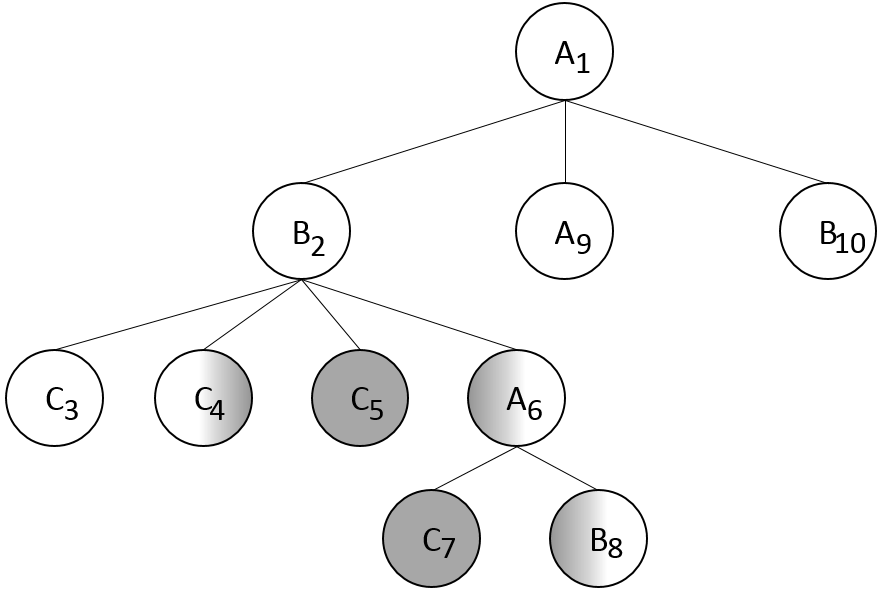
\includegraphics[scale=0.3]{figures/exampletree.png}
	\caption{An example XML tree} \label{fig:exampletree}
	\centering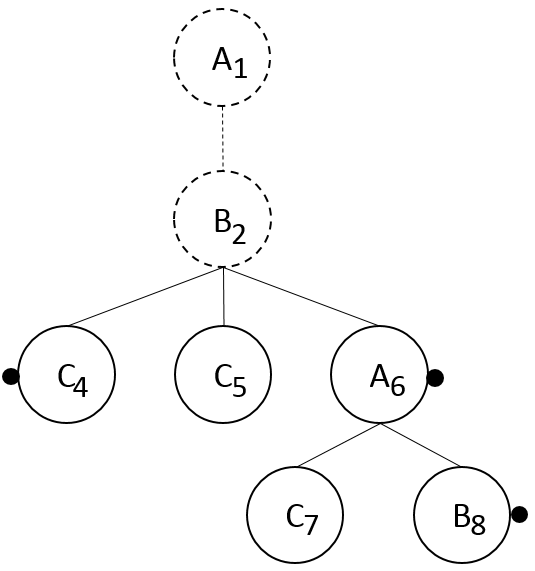
\includegraphics[scale=0.3]{figures/examplepartialtree.png}
	\caption{An example partial tree.} \label{fig:examplepartialtree}
\end{figure}

To address on the above two problems, we first proposed a novel tree structure,
called partial tree. As show in Figure 1.2.  We can create a partial tree for
the chunk. The partial tree has the information  of the missing path, i.e. A1
and B2. This tree is different from ordinary trees  because we define some
special nodes for partial tree (These special nodes with  dots in the feature
will be discussed at length in Section~\ref{sec:partialtree}).

By adding the nodes on the path from the root to the current chunk part, we are
now able to apply the queries to this partial tree based on the parent-child
relationships. We will discuss the query algorithms in
Section~\ref{sec:queryalgo}. Although partial tree is available in both
shared-/distributed- memory environments, it is more specially designed for
distributed-memory environments. This is becuase chunks of an XML documents can
distribted to multiple computers and then be parsed into partial trees for
further parallel processing.

\section{Contributions}

We consider two key contributions in the thesis.

The first contribution is the approach showing how to parallelize XPath queries
over fragmented XML documents stored in a number of XML databases, which also
involves implementations of~\cite{BoLS09}, our observations and perspectives
from the experiment results. Our implementations are designed for the
parallelization of XPath queries on top of BaseX, which is a state-of-the-art
XML database engine and XPath/XQuery 3.1 processor. With these implementations,
XPath queries can be easily parallelized by simply rewriting XPath queries with
XQuery expressions. We conduct experiments to evaluate our implementations and
the results showed that these implementations achieved significant speedups over
XML documents sized several gigabytes. Besides the experiment results, we also
present significant observations and perspectives from the experiment results.

The second contribution is the design of a novel tree structure, called partial
tree, for parallel XML processing. With this tree structure, we can split an XML
document into multiple chunks and represent each of the chunks with partial
trees. We also design a series of algorithms for evaluating queries over these
partial trees. Since the partial trees are created from separated chunks, we can
distribute these chunks to computer clusters. In this way, we can run queries on
them in distributed memory environments. We also proposed an efficient
implementation of partial tree. Based on indexing techniques, we developed a
indexing scheme, called BFS-array index along with grouped index. With this
indexing scheme, we can implement partial tree efficiently, in both memory
consumption and absolute query performance. The experiments showed that the
implementation can process 100s GB of XML documents with 32 EC2 computers. The
execution times were only seconds for most queries used in the experiments and
the throughput was approximately 1 GB/s.

\section{Outline}

The thesis is organized in six chapters. An introduction to this study is given
in Chapter 1. We  review the  related work in Chapter 2 and give definitions of
XML query languages in Chapter 3. We propose the idea of XPath queries on top of
BaseX in Chapter 4. We propose the new tree structure, partial tree in Chapter 5
and  we conclude the whole thesis in Chapter 6. Here are the detailed
introduction to the following Chapters.

Chatper 2

We discuss related work in three aspects: 1) XML fragmentation, which studies how
to fragment an single XML document tree into multiple sub documents trees, 2)
parallel evaluation of XML queries, which is about how to evaluate query on
fragmented XML data, and  3) XML database techniques, which is database
technology that are  closely to our study.

Chapter 3

In this section, the definitions of XML and two XML query languages: XPath and
XQuery used in this these are defined and we give introductions them to help
understand bases of this study.

Chapter 4

We introduce our approach of \cite{BoLS09} with the XML
processing engine BaseX. we also present our implementations and evaluate our
implementations on two data sets. Then, we propose our observations and 
perspectives from the experiment results. Based on them, we extend the study
to distributed-memory environment by introducing a fragmentation approach that
divides an XML document into fragments for parallel querying. 

Chapter 5

Firstly, we propose a noval tree structure called partial tree and give the 
definitions of partial tree and related items, discuss the characteristics 
and design querying algorithms over partial trees. Then, we propose an 
efficient BFS-index based implementation for partial tree. Lastly, we report 
and analyze the experiment results.

Chapter 6

We summarize this thesis and discuss the future work.



\chapter{Related Work} \label{sec:relatedwork}

We discuss related work in the following related fields, XML fragmentation,
parallel XML processing and XML database Techniques.

\section{XML Fragmentation} 

Fragmentation is characterized by physical changes to the dataset, that is, the
dataset is fragmented and allocated to multiple computational
nodes~\cite{BrMa14}. i.e. the process of dividing an XML document into multiple
smaller fragments. It is worth noting that the term $fragment$ refers to
well-formed XML document, which refers the potential of faster or more efficient
XML processing. It is generally the premise of data-parallel computation
algorithms. When process large XML documents, it is a natural way to reduce the
sizes of XML documents processed at a time, so that we can process them in
parallel to boost the perform of parsing and querying. For these reasons,
fragmentation has been intensively studied~\cite{ARBM06,DaGP14,CFKL12,NEMH07,
OgTP13,LiZZ17, CFKL12,DaGP14}. Generally speaking, there are two kinds of
fragmentation defined by Kling et al.~\cite{kling11:dist_xml}, who modeled
fragmentation as horizontal and vertical in terms of XML schema~\cite{schema}
that is a language for defnining the strucutre of XML documents by constraints. 

\subsubsection{Horizontal Fragmentation} \label{sec:hfragment}

Horizontal fragmentation is to divide a document tree into multiple fragments
and each fragment follows the same schema of the original XML document. When
fragments follow the same schema, they usually have similar structure.  Let us
take the tree in Fig.~\ref{fig:hfrag_example} as an example. We fragment the
tree into five subtrees, i.e. $d_1$, $d_2$,..., $d_5$ in the dotted rectangleds.
According to the schema, node `b' has a single `e' followed by one or zeor  `f';
node `c' has exact one `e'; node `d' can have zero or multiple node `g's. Thus,
all the subtrees follow the schema in Fig.~\ref{fig:hfrag_example}(b). Note that
all the fragments are ate the same level, which is a intuitive reason why the
fragmetation is called horizontal fragmetation.


\begin{figure}[t]
	\centering
	\begin{subfigure}{.6\textwidth}
		\centering
		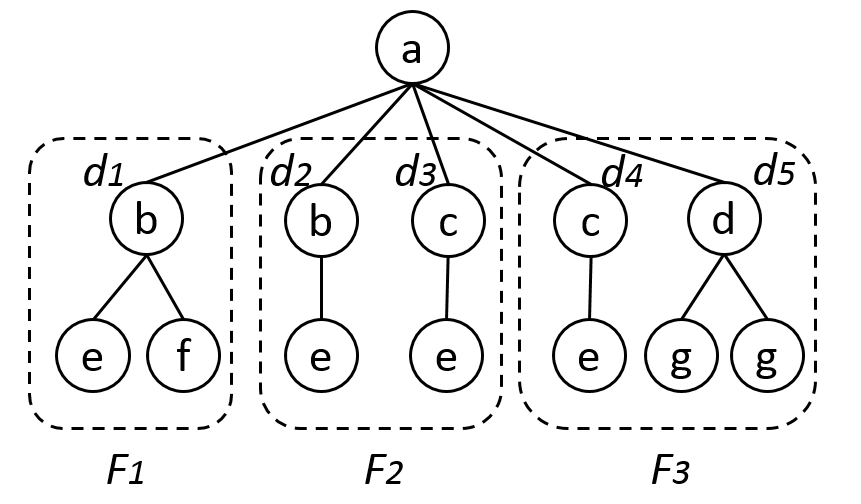
\includegraphics[width=.99\linewidth]{figures/hfrag_example}
		\caption{An example of horizontal fragmentation}
		\label{fig:sub1}
	\end{subfigure}%
	\begin{subfigure}{.4\textwidth}
		\centering
		\vspace{12mm}
		\begin{tabular}{|l|}
			\hline
			schema\\
			\hline
			a(b*, c*, d) \\
			b(e, f?) \\
			c(e) \\
			d(g*) \\
			\hline
		\end{tabular}
		\vspace{12mm}
		\caption{The schema of the example}
		\label{fig:sub2}
	\end{subfigure}
	\caption{An example of horizontal fragmentation and the schema.}
	\label{fig:hfrag_example}
\end{figure}


We then consider the whole document is a simple collection of fragments. Since
the fragments follow the same schema, the queries can be evaluated on them by
considering the schema. Horizontal fragmentation is rather straightforward and
thus widely used in parallel XML processing~\cite{DaGP14,BoLS09,AfDG15,CCMN15}.
In our study, we exploit and extend the horizontal fragmentation. 

\subsubsection{Vertical Fragmentation * To be extened.} \label{sec:vfragment}

Vertical fragmentation, on the other hand, is a fragmentation that extracts
subtrees from the middle of the tree, thus following different schemas. Though
this fragmentation does not usually work well for parallel XML processing, it is
worth studying. This is because it is a possible and  important in case when the
data are integrated from different sites or organizations~\cite{CFKL12,KlOD10}.
Thereare some studied followed this fragmetation.  Bose et al. proposed a
fragmentation model~\cite{bose2003query}. Bese on this, they later proposed a
system called Xfrag~\cite{bose2005xfrag}. In this system, an document is divided
into multiple sub documents called fillers, where other fragments (the fillers)
may fit.  Cong et al.~\cite{CFKL12} and Nomura et al. \cite{NEMH07} adopted a
tree-shaped fragment that contains original nodes and hole nodes, where a hole
node represents a link to a missing subtree, and represented the whole document
as a tree of fragments. The key part of their approaches to decouple
dependencies between evaluations on fragments so as to perform them in parallel. 

\section{Parallel XML Processing (Related to my parsing)}
\label{sec:paralleleval}

Many existing studies address the topic of XML processing in
parallel~\cite{BoLS09,PaZC08,LuGa08,Mats09,SAFu05}. We discuss parallel XML
processing in this section.

\subsection{Tree Accumulation and Reduction}

There are some exsisting ideas of dividing the XML documents and running the
computation for trees called tree reduction. Kakehi et al.~\cite{KaME07} showed
a parallel tree reduction algorithm from the nodes in chunks. Based on the idea
given by Kakehi et al., Emoto and Imachi~\cite{EmIm12} developed a parallel tree
reduction algorithm on Hadoop, and Matsuzaki and Miyazaki~\cite{MaMi16}
developed a parallel tree accumulation algorithm. A similar approach was taken
by Sevilgen et al.~\cite{SAFu05} who developed a simpler version of tree
accumulations over the serialized representation of trees.

\subsection{XML Streaming}

Stream processing is a possible approach for (parallel) online data analysis.
Parallel algorithms have been studied to accelerate stream processing of large
XML data. For example, XMLTK~\cite{AGGR02} is an XML stream processing tool
designed for scalable XML querying. Y-Filter~\cite{ZhPC10} applies multiple
queries in parallel for a stream of XML data. Among these studies, Ogden et
al.~\cite{OgTP13} achieved the highest throughput, 2.5 GB/s, based on the
parallel pushdown transducer. Although it is faster than our implementation of
partial tree, which is 1 GB/s, the class of queries we support is more
expressive than that of PP-transducer, which does not support order-aware
queries. In parallel pushdown transducers \cite{LiZZ17}, a given document is
modeled as a sequence of matched brackets and a fragment is represented as a
sequence of unmatched brackets.

\section{XML Parsing}

XML Parsing is a process of creating an XML tree from reading an XML document.
\cite{PLZC07,WZYu08} focused on XML parsing, which is related to our parsing
algorithm. Yinfei et al.~\cite{PaZC08} developed an algorithm for parsing the
XML data in parallel without any sequential preparsing phase.

Compared to these fragmentation techniques on trees, the fragmentation in this
study is based on serialized text, which means we cast the fragmentation on the
plain text of an XML document in stead of the XML tree parsed from the document.
The main advantage of our text-based fragmentation is that we can assign the
chunks over distributed file systems~\cite{dfs} that are cut by default. Similar
idea was introduced by Choi et al.~\cite{ChLL14} in which they added labels to
make every chunk a well-formed tree in a preparsing phase. 

\subsection{MapReduce-based XML Processing} \label{sec:mapreduce}

MapReduce~\cite{DeGh04} is a promising approach to large-scale XML processing,
which can run on top of clusters of commodity computers. It is suitalbe for
scalability as the size of XML data increases very rapidly.
Hadoop~\cite{HadoopWhit12}, which is a porpular implementtation of MapReduce, is
a common infrastructure for large-scale data processing, and to parallel
streaming~\cite{OgTP13,LiZZ17}. There have been several studies in this
direction~\cite{BCMU13,CFKL12,DaGP14,EmIm12,DaGP14,MaMi16}. One of earlier work
is by Choi et al.~\cite{CLKL12} called HadoopXML, which processes XML data in
parallel by applying SAX~\cite{sax} for each chunk. Including this work, most of
the existing MapReduce-based frameworks supports a small subset of XPath with
\texttt{child} and \texttt{descendant} axes with
predicates~\cite{CCMN15,AfDG15,DaGP14,DaGK14}. Instead, they extend the
expressiveness by the support of some query functionality (subsets of XQuery).
To cope with the problem of absolute performance of MapReduce, there is a few
work to use similar but more efficient frameworks, for example Apache
Flink~\cite{CCMN15}.

\subsection{Parallel Processing of queries}

Parallel XML processing has been actively studied after the paper presented by
Bordawekar et al.~\cite{BoLS09}, which closely relates to our study. The paper
proposes three strategies for XPath queries in parallel: data partition
strategy, query partition strategy, and hybrid partition strategy. . In fact,
there were some studies in the parallel programming community from 1990's.
Skillicorn developed a set of parallel computational patterns for trees called
tree skeletons, and showed they can be used for processing structured
documents~\cite{Skil97}. The main idea in parallelizing XPath queries was to
convert XPath queries into (tree) automata~\cite{comon2007tree}, and then
compute automata in parallel with tree skeletons. This idea was extended to
support a larger class of XPath including \texttt{following-sibling} by Nomura
et al.~\cite{NEMH07}. \cite{KrYa10,PLZC07,ZhPC10} focus on XPath queries
implemented in a shared-memory environment. \cite{AAHa11} proposed ideas about
XML processing in a forward and forward manner, which is helpful for our
research to support backward and upward queries as well. Liu et
al.~\cite{LFLQ08} developed a parallel version of structural join algorithm. The
study~\cite{ZaBS15} focuses processing a locality-aware partitioning in parallel
database systems. Cong et al.~\cite{CFKL12} formalized parallel processing of
XPath queries using the partial evaluation technique: the idea existing behind
their partial evaluation is similar to automata.

\section{XML Database Techniques}

\subsection{Indexing and Labeling Schemes}

Indexing is a commom database technique to improve the access of data  by using
index. It is also useful to for accelerating the access in XML databases.
However, due to the tree structure, it is a challenge to create efficient  index
for XML documents. In the early 2000, O'Neil et al.~\cite{OOPC04} proposed an
index called ORDPATH for natively supporting XML data type. This index makes it
possible to process XML queries inside the database with downward XPath queries
and allows update operations. Since this length of this index increases with
respect to the size of XML documents, the length will be very long in case the
XML documents are large. Pal et al.~\cite{PCSS04} studied how to improve the
query performance by introducing two indexes to nodes and values in SQL
Server~\cite{sql2005}. Li et al~\cite{LiLi05} improved OrdPath by reducing the
length of ORDPATH index when inserting. Min et al.~\cite{MLCh07} proposed an
efficient labeling scheme, called EXEL, which incurs no re-labeling of nodes
when inserting nodes. Finis et al~\cite{FBKF15} Proposed an idea mainly on how
to maintain and query hierarchical data at a high rate of complex, possibly
skewed structural updates. There indexes inspire our deisgn of index scheme on
XML document to make ours in a more efficient way. There are also some studyies
concerning specific types of trees, such as \cite{ToGr02,JLWO03,CVZZ08}, whicsh
examined the differences in indexing trees, including B+-tree, R-tree, and
XR-tree. In this theses, by  considering the above studies, an new conbimed
index is designed for specially  for large XML data.

\subsubsection{Joins Algorithms}

Join processing is central to database implementation~\cite{graefe1993query}.
There are two join algorithms commonly used in XML processing, structural join
and twig join.

Structural join~\cite{AlJYK02} is mostly based on numbering
indexing\cite{numbering}, which numbers a nested intervals on nodes and is
commonly used in XML and other database
applications~\cite{ZNDI01,HAJR03,ZNDI01}. By using the information of start
position, end position and level of each node, the parent-child and
ancestor-descendant relationships of nodes can be determined by a merge join on
two lists of nodes. In 2001, a earily study~\cite{LiMo01} proposed three joint
algorithms for processing XML queries, which were similar to structural join. In
2002, Quanzhong Li et al. first proposed structural join in~\cite{AlJYK02}.
Jiang et al.~\cite{JLWO03} improved the structural join with a novel tree
structure, called XR-tree, which is suitable for identifying the descendants of
a given node with optimized worst case I/O cost. Le Liu et al.~\cite{LFLQ08}
first applied structural join in parallel over shared-memory environments.

Twig joins are also commonly used for maching a part of an XML
documents~\cite{jiang2003holistic,lu2005efficient,lu2005tjfast,
fontoura2005optimizing}. In twig join, a query is represented as a twig patten,
and then is searched on the target XML document. One of the early twig joins was
\cite{BrKS02}. In the paper, a holistic twig join algorithm, called TwigStack
was proposed for matching an XML query. There are also variants of twig joins
then devleoped~\cite{CLTH06,QiYD07}. In 2009, Machdi et al.~\cite{MaAK09}
implemented the idea in parallel on multiple cores and in 2012 Choi et
al.~\cite{CLKL12} studied the twig joins on Hadoop in a parallel manner.






\chapter{XML and Query Languages}

In this chapter, we introduce XML and two query languages: XPath
and XQuery, used in this study.


\section{XML}

XML~\cite{XML} is a standard data describing language used for representing
arbitrary data in a hierarchical structure. As introduced, XML
documents are increasing dramatically in size over time. Large XML documents in
this thesis refer to XML documents whose sizes are greater than 1 gigabytes.

Each XML document corresponds to a logical XML tree (or simply tree) that
contains one or more elements.  There are several types of elements in the tree
of an XML document. In this study, we focus on the following three element
types.

\begin{itemize}
	\item Element node \\
	An element node is parsed from a pair of tags, a start tag and a end tag, and
	are used to represent the structure of an XML tree. All element nodes are
	ordered as their corresponding tags appear in the XML document.
	\item Content node \\
	A content node (also called value node) represents the value of a element node.
	\item Attribute node \\
	An attributes node is used to associate name-value pairs inside a start tag of
	an element node for describing properties of the element node.
\end{itemize}

% Nodes are ordered.

Now, we give an example to show what these nodes are. Given the following
XML text string.\\

\hspace{10ex}\texttt{<A>}

\hspace{14ex}\texttt{<B AT1="VAL1">TXT1</B>}

\hspace{14ex}\texttt{<D>}

\hspace{18ex}\texttt{<E AT2="VAL2"></E>}

\hspace{18ex}\texttt{<F>}

\hspace{22ex}\texttt{<G>}

\hspace{26ex}\texttt{<I></I>}

\hspace{22ex}\texttt{</G>}

\hspace{22ex}\texttt{<H>TXT2</H>}

\hspace{18ex}\texttt{</F>}

\hspace{18ex}\texttt{<J></J>}

\hspace{14ex}\texttt{</D>}

\hspace{14ex}\texttt{<K>}

\hspace{18ex}\texttt{<L>TXT3</L>}

\hspace{14ex}\texttt{</K>}

\hspace{10ex}\texttt{</A>}\\

We can create an XML tree as shown in Figure~\ref{fig:relationships} (The
example of three element types are shown on left-bottom corner). For example,
the node B is an element node. There two nodes below B and are connected to it.
The left one  is an attribute node with the name `AT1' and the value `VAL1'. The
right  one is a value node with the string value `TXT1'.

\begin{figure}[t]
	\centering
	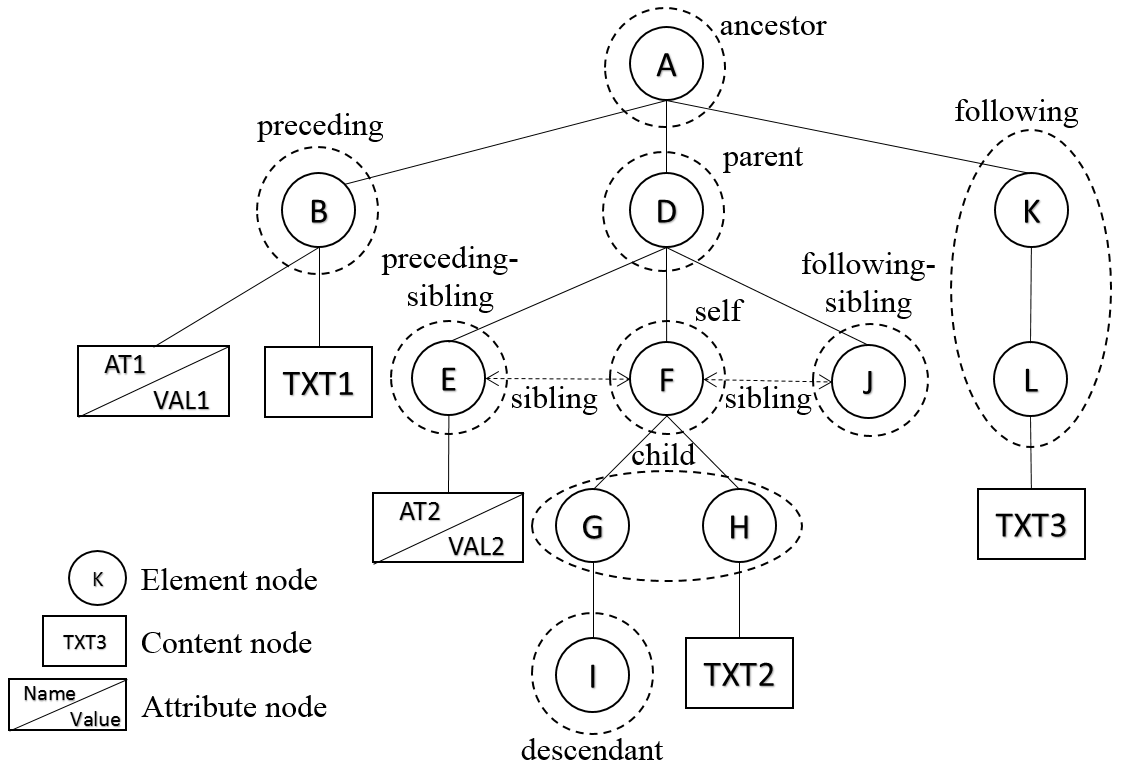
\includegraphics[width=1\linewidth]{figures/relationships}
	\caption{An example of node relationships.}
	\label{fig:relationships}
\end{figure}



\section{XPath Language}
\label{sec:xpath}

\subsection{Definition of XPath}

XPath is an XML query language used for selecting parts of an XML
document~\cite{xpath}. XPath queries are represented in path expressions. Each
path expression contains one or more \emph{location steps} or simply
\emph{stpes}. In this study, each step consists of an \emph{axis}, a \emph{name
test}, and at most one \emph{predicate}.

An axis defines the relationships of the current node and the target nodes.
There are 12 axes supported in this study, including  \texttt{child},
\texttt{descendant}, \texttt{parent}, \texttt{ancestor},
\texttt{descendant-or-self}, \texttt{ancestor-or-self}, \texttt{following},
\texttt{following-sibling}, \texttt{preceding}, \texttt{ preceding-sibling}  and
\texttt{attribute}. Note that \texttt{attribute} is different from the the other
axes. Because it selects only attribute nodes, while the other axes select only
element nodes. Content nodes can be selected by using function \texttt{text()}.
Figure~\ref{fig:relationships} uses node F as the current node to demonstrate
these axes. In the figure, F has a parent D, two siblings: E  on the left side
as a preceding-sibling and I on the right side as a following sibling, two
children: G and H, one descendant I, one preceding B, and two followings: nodes
K and L.

A name test is used for selecting nodes. If the name of a tag in an XML document
is equal to the name test, the node is selected. XPath also defines a wilecard  `*'
that matches with any name.

A predicate written between ``\verb|[|'' and ``\verb|]|'' describes additional
conditions to filter the matched nodes by using a path.

For example, given a query
``\verb|/descentdant::F[following-sibling::J]/child::H|'', this XPath query has
two steps where \verb|descendant| and \verb|child| are the axes, \verb|F| and
\verb|H| are the name tests, and a predicate \verb|child::H| is attached to the
second step.

\subsection{Evaluting XPath query}


\begin{figure}[!t]
	\centering\fbox{
		\begin{minipage}{.95\linewidth}
			\textit{Query} ::= `\texttt{/}' \textit{LocationPath}          \\
			\textit{LocationPath} ::= \textit{Step} $~|~$ \textit{Step} `\texttt{/}' \textit{LocationPath}          \\
			\textit{Step} ::= \textit{AxisName} `\texttt{::}' \textit{NameTest} \textit{Predicate}?          \\
			\textit{AxisName} ::= `\texttt{self}' $~|~$ `\texttt{child}' $~|~$ `\texttt{parent}'   $~|~$ `\texttt{descendant}'   $~|~$ `\texttt{ancestor}'          \\
			\phantom{\textit{AxisName} :}  `\texttt{descendant-or-self}' $~|~$ `\texttt{ancestor-or-self}'  $~|~$ `\texttt{following}'    \\
			\phantom{\textit{AxisName} :}        $~|~$ `\texttt{following-sibling}'  $~|~$ `\texttt{preceding}  $~|~$ `\texttt{preceding-sibling}'          \\
			\phantom{\textit{AxisName} :}        $~|~$ `\texttt{attribute}'   \\
			\textit{NameTest} ::= `\texttt{*}' $~|~$ \textit{string}	          \\
			\textit{Predicate} ::= `\texttt{[}' \textit{SimpleLocationPath} `\texttt{]}'          \\
			\textit{SimpleLocationPath} ::= \textit{SimpleStep} $~|~$ \textit{SimpleStep} `\texttt{/}' \textit{SimpleLocationPath}          \\
			\textit{SimpleStep} ::= \textit{AxisName} `\texttt{::}' \textit{NameTest}
		\end{minipage}
	}
	\caption{Grammars of XPath queries used for partial tree}
	\label{fig:grammar}
\end{figure}


When evaluating an XPath query, we start from the first step and evaluate each
location step in order. When meeting a predicate, we process it as a filter to
rule out unmatched nodes. Let us continue to use the query above to demonstrate.
This query first retrieves all the nodes with name \verb|F| in a XML document,
and then among their children it retrieves node \verb|H| with one or more
children with name \verb|J|. In other words, the result of the query is a set of
nodes \verb|H|, each of which has its parent \verb|F| and at least one sibling
\verb|G| on its right. The grammar of XPath used in this study for our novel
tree structure partial tree (See Chapter~\ref{ch:partialtree}) is listed in
Figure~\ref{fig:grammar}.


\section{XQuery}

XQuery is also a language for querying XML documents. It for XML is like SQL for
databases. It integrates with XPath language and an XPath query in an XQuery
expression returns exactly the same result as in XPath language. XQuery is more
expressive and powerful (also more complicated) than XPath.  Now, let use
consider the following expression as an example. In this study, we used XQuery
3.1~\cite{XQuery3_1}.

\begin{lstlisting}
for $x in doc("books.xml")/bookstore/book
return $x/title
\end{lstlisting}

This XQuery expression queries an XML document, namely ``books.xml''. It
evaluates an XPath query \texttt{/bookstor/book} over the document to select all
\texttt{book} of the root \texttt{bookstore} and returns the \texttt{title} of
the selected \texttt{book}.

\section{Summary}

In this chapter, we have introduced three languages used in this thesis: XML,
XPath and XQuery. XML is used to represent arbitrary data. Data stored in XML
format are called XML document. XPath and XQuery are languages for querying XML
documents. XQuery integreates with XPath and thus is more powerful and
expressive.

% as the XML query language  for maniulating XPth queries on top of
% BaseX~\cite{basex864} by utilizing some features and functions of XQuery 3.1,
% such as arrays and XQuery Update Facility. Moreover, we exploit XQuery
% extension for full-text operations, particularly the function
% \texttt{ft:tokenize} for converting a string into a string array.


\newcommand{\Placeholder}[1]{$\langle\!\langle\mbox{\textrm{#1}}\rangle\!\rangle$}
\newcommand{\bfn}[1]{\textup{#1}}
\newcommand{\Src}[1]{\texttt{#1}}
\newcommand{\fn}[1]{\mathit{#1}}
\newcommand{\modify}[3]{{\underline{\sf{#1}}:} {\color{blue}{#2}} {\color{green}{\mbox{$\Rightarrow$}}} {\color{red}{#3}}}
\newcommand{\todo}[2]{{\underline{\textsf{#1}}:} {\color{red}{$\spadesuit$#2$\spadesuit$}}}
\newcommand{\hack}{{\color{red}{$\blacklozenge$}}}


\chapter{Parallelization Of XPath Queries on Top of BaseX}

On the topic of parallelelization of XPath queires, one practical and promising
approach was proposed by Bordawekar et al.~\cite{Bord10} in 2009. In this study,
three partitioning strategies were presented, i.e. data partitioning, query
partitiooning  and hybrid partitioing startegies,  making it possible to
parallelize XPath queries by partitioning an XPath query into subqueries and
evaluating them in parallel on XML trees.

However, since this study was based on an XSLT processing, it is thus not clear
to the following questions: \textit{(1) Whether and how can we apply their
partitioning strategies to XML database engines? (2) What speedup can we achieve
on large XML documents?}.

To answer the above two questions, we introduce our implementations on top of a
state-of-the-art XML database engine BaseX with two large XML documents sized 
1.1 GB and 1.85 GB by reviving and extending Bordawekar et al's study. We propose
three implementations on the base of the original idea from the paper and we also
extended our implementations in term of BaseX by exploiting its optimizations.
We experimentally demonstrate the performance on top of BaseX with two large 
XML documents. The experiment results proved that it is
possible to obtain significant speedups by simply rewriting queries into
subqueries and parallelizing the evaluation of them on top of an XML database
engine over gigabytes of XML documents, without need to modify source code of the engine.

%\input{basex/partitions}

\section{BaseX: An XML Database Engine}
\label{sect:basex}

To begin with, we give a brief introduction to BaseX, which is both a
state-of-the-art XML database and an XQuery/XPath 3.1 processor (refer to the
official documentation~\cite{basex864} for more details). BaesX provides
significant features in processing XML data sets. The following are the BaseX's
features particularly important for our study:

\begin{itemize}
	\item Full support of XQuery 3.1, especially arrays and XQuery Update Facility;
	\item XQuery extension for database operations, especially index-based
	random access;
	\item XQuery extension for full-text operations, especially
	\Src{ft:tokenize};
	\item Support of in-memory XML databases;
	\item Query optimization based on various indices.
	\item Support of concurrent transactions in the server mode.
\end{itemize}

The first three are concerned with the expressiveness of queries and the rests
are concerned with performance.

The most important (practically essential) feature to our implementations is
index-based random access to nodes of an XML database in BaseX. BaseX offers
indices that enable us to access any node in constant time. The PRE index, which
denotes the position of a node in the document order, brings the fastest
constant-time access in BaseX. Function \Src{db:node-pre} returns the PRE value
of a given node and function \Src{db:open-pre} returns the node of a given PRE
value. For example, given a BaseX database ``exampledb'', as shown below.
\begin{lstlisting}[escapechar=\@]
@$^1$@<books>
  @$^2$@<book>
	 @$^3$@<name>@$^4$@XML</name>
	 @$^5$@<author>@$^6$@Jack</author>
  @$^{\phantom{3}}$@</book>
@$^{\phantom{1}}$@</books>@\textrm{~,}@
\end{lstlisting}
where a left superscript denotes a PRE value. Now, consider the following query.
\begin{lstlisting}
for $node in db:open(``exampledb'')/books/book
return db:node-pre($node)
\end{lstlisting}
The querys selects \texttt{book} in `exampledb' and the result of \texttt{\$node} is
\verb|<book>...</book>|. Then, after applying the \texttt{db:node-pre} function
the final result is 2. PRE values are well-suited for representing intermediate
results of XPath queries because a PRE value is merely an integer that makes it
efficient to restart a tree traversal with PRE values. Letting a PRE value be 2
on the `exampledb', we use the following query as an example.

\begin{lstlisting}
for $pre in db:open-pre(``exampledb'', 2)/author
return $node
\end{lstlisting}

The \texttt{db:open-pre} takes the database and PRE as arguments to locate the
\texttt{book} node. Then it selects the \texttt{author} of \texttt{book}. The final
result is \verb|<author>Jack</author>|.


Arrays are useful for efficiently implementing block partitioning. On BaseX, the
length of an array is returned in constant time and the subarray of a specified
range is extracted in logarithmic time\footnote{In fact, both sequences and
arrays on BaseX are implemented with finger trees and therefore the
corresponding operations on sequences have the same cost.}. XQuery Update
Facility over in-memory databases strongly supports efficient use of temporary
databases for holding results of queries. Function \Src{ft:tokenize}, which
tokenizes a given string to a sequence of token strings, can implement
deserialization of sequences/arrays efficiently.  

BaseX's query optimization is so powerful that it is not unusual to improve time
complexity. For example, path index enables pruning
traversal of descendants and attribute index enables instant access to
the nodes that have a specific attribute name or value. With aggressive constant
propagation, BaseX exploits most constants including database metadata and PRE
values found in a given query for query optimization. Prevention of spoiling it,
as to be described in Section~\ref{sect:opt}, is therefore of crucial importance
for performance.

Lastly, BaseX can work in a client-server mode. A BaseX server can handle
concurrent transactions requested from BaseX clients with multiple threads
depending on the server's configurations. Read transactions that do not modify
data, such as XPath queries, are executed in parallel without waiting or using
locks in BaseX.


\section{Implementing Data Partitioning with BaseX}
\label{sect:dpsimpl}

In this section, we describe our two implementations for data partitioning
strategy, namely the client-side implementation and the server-side
implementation, on top of BaseX.

Data partitioning is to split a given query into a prefix query and a suffix
query, e.g., from \texttt{$q_1$/$q_2$} to prefix $q_1$ and suffix $q_2$, and to
run the suffix query in parallel on each node of the result of the prefix query.
The results of suffix queries are concatenated in document order to form the 
final result.


Our implementations are Java programs that involve a BaseX client. They
spawn $P$ threads (usually P is no more than the number of physical cores) and 
create a connection to a BaseX server for each thread so
as to run multiple queries in parallel after a prefix query. Merging $P$ partial
results in the form of string is sequentially implemented. The main difference
between the client-side and the server-side implementations is the way how the results of prefix
queries are handled. In the rest of this section, we describe them by using
XM3(a) shown in Table~\ref{tab:dpsqueries} as a running example, assuming input
database to be named \Src{`xmark.xml'}.

\subsection{Client-side Implementation}

The client-side implementation is a simple implementation of data partitioning
strategy with database operations on BaseX. It sends the server a prefix query 
to be executed and the PRE values of matched nodes are returned. The
following XQuery expression is used for the prefix query of XM3(a).

\begin{lstlisting}
for $x in db:open(``xmark'')/site//open_auction
return db:node-pre($x)
\end{lstlisting}

Let this prefix query return sequence \Src{(2, 5, 42, 81, 109, 203)}. 
Letting $P = 3$, it is block-partitioned to \Src{(2, 5)}, \Src{(42,
81)}, and \Src{(109, 203)}, each of which is assigned to a thread. To avoid
repetitive ping-pong between a client and the server, we use the following
suffix query template:

\vspace{10mm}
\begin{lstlisting}[escapechar=\@]
for $x in @\Placeholder{sequence of PRE}@
return db:open-pre(``xmark'', $x)/bidder[last()]@\textrm{~,}@
\end{lstlisting}
where \Placeholder{sequence of PRE} is a placeholder to be replaced with a
concrete partition, e.g., \Src{(42, 81)}. Each thread instantiates this template
with its own partition and sends the server the instantiated query.


\subsection{Server-side Implementation}

A necessary task on the results of a prefix query is to block-partition them.
The client-side implementation simply processes it on the client side. In fact,
we can also implement it efficiently on the server side by utilizing BaseX's
features.

First, we prepare an in-memory database named \Src{``tmp''} and initialized with
\Src{<root> </root>}, which is a temporary database for storing the results of a
prefix query.  The prefix query is \texttt{/site//open\_auction} and it selects 
all \texttt{open\_auction} and return the PRE values of matched nodes. 
It is implemented as follows:

\begin{lstlisting}[escapechar=\@]
let $P := @\Placeholder{number of partitions}@
let $arr := array { for $x in db:open(``xmark'')/site//open_auction
                       db:node-pre($x) }
for $i in 1 to $P
return insert node element part { $block_part($i, $P, $arr) }
         as last into db:open('tmp')/root@\textrm{~,}@
\end{lstlisting}
where \Placeholder{number of partitions} denotes a placeholder to be replaced
with a concrete value of $P$ and \verb|$block_part($i, $P, $arr)| denotes the
\verb|$i|-th subarray of \verb|$P|-block partitioned \verb|$arr|. With the array
operations of extracting length and subarray, \verb|$block_part| is implemented
in logarithmic time.

In the example case used earlier, \Src{``tmp''} database results in the following:
\newpage
\begin{lstlisting}[escapechar=\@]
@$^1$@<root>
  @$^2$@<part>@$^3$@2 5</part>@$^4$@<part>@$^5$@42 81</part>@$^6$@<part>@$^7$@109 203</part>
@$^{\phantom{1}}$@</root>@\textrm{~,}@
\end{lstlisting}
where a left superscript denotes a PRE value. Note that its document structure
determines the PRE value of $i$th partition to be $2i+1$.

A suffix query is implemented with deserialization of a partition as follows:
\begin{lstlisting}[escapechar=\@]
for $x in ft:tokenize(db:open-pre(``tmp'', @\Placeholder{PRE of partition}@))
return db:open-pre('xmark', xs:integer($x))/bidder[last()])@\textrm{~,}@
\end{lstlisting}
where \Placeholder{PRE of partition} denotes a placeholder to be replaced with
the PRE value of a target partition.

In most case, the server-side implementation is more efficient because communication data
between clients and a server except for output is reduced to a constant size.


\begin{figure}[tbp]
	\centering
	\caption{List of XPath queries and their partitioning, where pre and suf
		mean prefix query and suffix query respectively}
	\label{tab:dpsqueries}
	\small
	\begin{tabular}{l|l}
		\hline
		Key & Query \\
		\hline
		XM1  & \verb|/site//*[name(.)="emailaddress" or name(.)="annotation" or| \\
		& \verb| name(.)="description"] |\\
		XM1(a) & pre = \verb|/site/*|, \\
		& suf = \verb|descendant-or-self::*[name(.)="emailaddress" or | \\
		& \verb|     name(.)="annotation" or name(.)="description"]| \\
		\hline
		XM2 & \verb|/site//incategory[./@category="category52"]/parent::item/@id| \\
		XM2(a) & pre = \verb|/site//incategory|, \quad \\
		& suf = \verb|self::*[./@category="category52"]/parent::item/@id| \\
		XM2(b) & pre = \verb|/site/*|, \quad  \\
		& suf = \verb|descendant-or-self::incategory[./@category="category52"]|\\
		& \verb|      /parent::item/@id| \\
		XM2(c) & pre = \verb|db:attribute("xmark10", "category52")|, \\
		& suf = \verb|parent::incategory[ancestor::site/parent::document-node()]| \\
		& \verb|      /parent::item/@id| \\
		\hline
		XM3 & \verb|/site//open_auction/bidder[last()]| \\
		XM3(a) & pre = \verb|/site//open_auction|, \quad suf = \verb|bidder[last()]| \\
		XM3(b) & pre = \verb|/site/*|, \quad \\
		& suf = \verb|descendant-or-self::open_auction/bidder[last()]| \\
		XM3(c) & pre = \verb|/site/open_auctions/open_auction|, \quad suf = \verb|bidder[last()]| \\
		\hline
		XM4 & \verb|/site/regions/*/item[./location="United States" and ./quantity > 0| \\
		& \verb| and ./payment="Creditcard" and ./description and ./name]| \\
		XM4(a) & pre = \verb|/site/regions/*|, \quad\\
		& suf = \verb|item[./location="United States" and ./quantity > 0 and | \\
		& \verb|     ./payment="Creditcard" and ./description and ./name]| \\
		XM4(b) & pre = \verb|/site/regions/*/item|, \quad \\
		& suf = \verb|self::*[./location="United States" and ./quantity > 0 and|  \\
		& \verb|     ./payment="Creditcard" and ./description and ./name]| \\
		XM4(c) & pre = \verb|db:text("xmark10", "Creditcard")/parent::payment|, \\
		& suf = \verb|parent::item[parent::*/parent::regions| \\
		& \verb|      /parent::site/parent::document-node()]| \\
		& \verb|     [location = "United States"][0.0 < quantity][description][name]| \\
		\hline
		XM5 & \verb|/site/open_auctions/open_auction/bidder/increase| \\
		XM5(a) & pre = \verb|/site/open_auctions/open_auction/bidder|, \quad suf = \verb|increase| \\
		XM5(b) & pre = \verb|/site/open_auctions/open_auction|, \quad suf = \verb|bidder/increase| \\
		\hline
		XM6 & \verb|/site/regions/*[name(.)="africa" or name(.)="asia"]| \\
		&  \verb|/item/description/parlist/listitem| \\
		XM6(a) & pre = \verb|/site/regions/*|, \quad \\
		& suf = \verb|self::*[name(.)="africa" or name(.)="asia"]|\\
		& \verb|     /item/description/parlist/listitem| \\
		XM6(b) & pre = \verb|/site/regions/*[name(.)="africa" or name(.)="asia"]/item|, \quad  \\
		& suf = \verb|description/parlist/listitem| \\
		\hline
		DBLP1 & \verb|/dblp/article/author|\\
		DBLP1(a) & pre = \verb|/dblp/article|,   suf = \verb|author|\\
		\hline
		DBLP2 & \verb|/dblp//title|\\
		DBLP2(a) & pre = \verb|/dblp/*|,  suf = \verb|self::*//title|\\
		\hline
	\end{tabular}
\end{figure}


\section{Implementing Query Partitioning with BaseX}
\label{sect:qpsimpl}

In this section, we describe our implementation of query partitioning strategy on top of
BaseX. The implementation of query partitioning strategy is also a Java program that
involves a BaseX client. This implementation
is relatively simpler than that for data partitioning.  It has two-phase, 
a parallel evaluating phase and a merge phase.  In the
parallel evaluating phase, a query is divided into multiple subqueries, which 
are executed by a BaseX server in parallel. In the second phase,
the results of all subquery are merged together into a whole as the final
result. In the following paragraphs, we focus the parallel evaluating phase 
of query partitioning in detail.


There are two ways of partitioning an XPath query in the
parallel evaluating phase: position-based partitioning and predicate-based
partitioning. Position-based partitioning is to divide the query by the
\texttt{position} function on a specific location step.  It is based on the
partition of children of a node in particular positions such that these children
are divided into multiple groups in order. Then, we evaluate on these groups of
nodes and its branches in parallel. Let us take XM5 as example. The children
nodes of \texttt{/site/open\_auctions} on `xmark10.xml' is 120000. Letting P =
3, then we can use the \texttt{position} function to divide the query into three
subqueries as follows:\\
\begin{small}
	\verb|/site/open_auctions\open_auction[position()=1 to 40000]\bidder/increase|\\
	\verb|/site/open_auctions\open_auction[position()=40001 to 80000]\bidder/increase|\\
	\verb|/site/open_auctions\open_auction[position()=80001 to 120000]\bidder/increase|\\
\end{small}
These three subqueries cover exactly the same parts on the target XML document 
as that of the original query and returns in turn the same results. 
Node that since the query is divided
by the \texttt{position} function in document order, the results are also in
document order. Thus, we can simply merge the results orderly to form the final
result.

% branch-based partitioning

As for the predicate-based partitioning, it is not promising to be introduced in
term of XML database engines. This is because it takes extra time to
merge the results of subqueries. For example, given a query \texttt{/q1[q2 or
	q3]} that is divided into \texttt{q1[q2]} and \texttt{q1[q3]}, we can retrieve
results from both queries. Since the operation is an `\texttt{or}', we need to
perform an ordered union to the results of the two subqueries. However, since
the resultant nodes in the results, there are two difficulties to merge them.
First, we need to determine the order of nodes in the results. Second, the
merging process itself is time-consuming when the results are in plain text.
Therefore, we do not discuss this partitioning in our study.

We also extend the query partitioning strategy by partitioning the children with
different names, called branch-based partitioning. We exploit the structure of the
input XML document to evaluate subqueries on the branches of a node by walking
through its children in parallel. Let us take XM1(d) on `\texttt{xmark10.xml}'
as an example. Since the root of the document has only six nodes:
\texttt{regions}, 
\texttt{categories}, 
\texttt{catgraph}, 
\texttt{people},
\texttt{open\_auctions},
\texttt{closed\_auctions}, 
we can make the input query into six corresponding sub
queries. Given the first child \texttt{regions} of the root, we make the
corresponding subquery as
\verb|/site/regions/descendant-or-self::incategory.../@id|, which is to be
evaluated through only the first branch of the root  and selects \texttt{@id}s
that matches the query in that branch. 
The six corresponding sub queries cover exactly the same part of the
original query and return the same results. Because the children of the root are
in document order, the results are also ordered as long as the results are
merged in the same order.


\begin{figure}[tbp]
	\centering
	\caption{List of XPath queries used for query partitioning, where [pos] denotes position-based partitioning and \{name\} denotes branch-based partitioning.}
	\label{tab:qpsqueries}
	\small
	\begin{tabular}{l|l}
		\hline
		XM1 & \verb|/site//*[name(.)="emailaddress" or name(.)="annotation"| \\
		& \verb| or name(.)="description"]|\\
		XM1(d) & \verb|/site/*[pos]/descendant-or-self::*[name(.)="emailaddress" |\\
		&  or name(.)="annotation" or name(.)="description"]| \\
		XM1(e) & \verb|/site/{name}/descendant-or-self::*[name(.)="emailaddress" |\\
		& \verb| or name(.)="annotation" or name(.)="description"]|\\
		\hline
		XM2 & \verb|/site//incategory[./@category="category52"]/parent::item/@id| \\
		XM2(d) & \verb|/site/regions/*[pos]/item/incategory[./@category="category52"]|\\
		& \verb|/parent| \\
		XM2(e) & \verb|/site/regions/{name}/item/incategory[./@category="category52"]|\\
		& \verb|/parent| \\
		\hline
		XM3 & \verb|/site//open_auction/bidder[last()]|\\
		XM3(d) & \verb|/site/open_auctions/open_auction[pos]/bidder[last()]|\\
		\hline
		XM4 & \verb|/site/regions/*/item[./location="United States" and ./quantity| \\
		& \verb| > 0 and ./payment="Creditcard"and ./description and ./name]|\\
		XM4(d) & \verb|/site/regions/*[pos]/item[./location="United States"|\\
		& \verb|and ./quantity > 0 and ./payment="Creditcard and ./description| \\
		& \verb|and ./name]| \\
		XM4(e) & \verb|/site/regions/{name}/item[./location="United States"|\\
		& \verb|and ./quantity > 0 and ./payment="Creditcard" and ]|\\
		& \verb|./description and ./name| \\
		\hline
		XM5 & \verb|/site/open_auctions/open_auction/bidder/increase| \\
		XM5(d) & \verb|/site/open_auctions/open_auction[pos]/bidder/increase|\\
		\hline
		XM5(e) & \verb|/site/open_auctions/open_auction/bidder[pos]/increase|\\
		\hline
		XM6 & \verb|/site/regions/*[name(.)="africa" or name(.)="asia"]| \\
		& \verb|/item/description/parlist/listitem| \\
		XM6(d) & \verb|/site/regions/*[pos][name(.)="africa" or name(.)="asia"]| \\
		& \verb|/item/description/parlist/listitem| \\
		XM6(e) & \verb|/site/regions/\{name\}[name(.)="africa" or name(.)="asia"]| \\
		& \verb|/item/description/parlist/listitem| \\
		\hline
		DBLP1 & \verb|/dblp/article/author| \\
		DBLP1(d) & \verb|/site/regions/*[pos][name(.)="africa" or name(.)="asia"]| \\
		& \verb|/item/description/parlist/listitem|\\
		\hline
		DBLP2 & \verb|/dblp//title| \\
		DBLP2(d) & \verb|/dblp/{name}/titlem|\\
		\hline
	\end{tabular}
\end{figure}


%In query partitioning, the position-based and branch-based partitions 
%in our study are the same, which evaluate a
%query through dividing the children of a node. There, however, still are three
%main differences between them. First, position-based partitioning is not
%sensitive to the number of children of a node, i.e. no matter how big or small
%the number of nodes is, it is always available in both cases. This is because
%the \texttt{position} function can process a range of nodes in a subquery. As
%for branch-based partitioning, it is usually feasible only in case when the
%number of children is small. This is because each child makes a sub query. Thus,
%when the number of children is too big, there are by too many subqueries and
%need too many threads that may excess the number of available threads. In
%additional, the overhead of parsing theses subqueries is dramatic. Third, the
%branch-based is more  likely to be limited to the structure of input XML
%document. This is because  in real world XML documents, it is more likely to be
%ill-balanced when the names  of children of a node are different.  


\section{Integration with Query Optimization}
\label{sect:opt}

As mentioned in Section~\ref{sect:basex}, BaseX is equipped with a powerful
query optimizer. Some queries can be optimized to reduce execute time. For
example, BaseX optimizes XM3 can be optimized as follows.

\begin{lstlisting}
/site/open_auctions/open_auction/bidder[last()]
\end{lstlisting}

This optimization is on the basis of the path index, which brings knowledge that
\Src{open\_auction} exists only immediately below \Src{open\_auctions} and
\Src{open\_auctions} exists only immediately below \Src{site}. Because a step of
descendant-or-self axis (\Src{//open\_auction}) is replaced with two steps of
child axes (\Src{/open\_auctions/open\_auction}), the search space of this query
has been significantly reduced. Note that a more drastic result is observed in
XM2, where the attribute index is exploited through function \Src{db:attribute}. 

Partitioning strategies convert a given query to two separate ones and therefore
affects the capability of BaseX in query optimization. In fact, the suffix query
of XM3(b) is not optimized to the corresponding part of optimized XM3 because
BaseX does not utilize indices for optimizing queries starting from nodes
specified with PRE values even if possible in principle. Most index-based
optimizations are limited to queries starting from the document root. This is a
reasonable design choice in query optimization because it is expensive to check
all PRE values obtained from the evaluation of a prefix query. However, we do
not have to check all PRE values that specify the starting nodes of the suffix
query because of the nature of data partitioning, of which BaseX is unaware.
This discord between BaseX's query optimization and data partitioning may incur
serious performance degradation, and it also occurs in query partitioning
strategy in term of parallelizing subquereis.

A simple way of resolving this discord is to apply partitioning strategies to
the suffix queries after BaseX's query optimization. Partitioning strategies are
applicable to any multi-step XPath query in principle. Even if an optimized
query is thoroughly different from its original query as in XM2, it is entirely
adequate to apply both partitioning strategies to the optimized query,
forgetting the original. In fact, XM2--4(c) are instances of such data
partitioning after optimization.

The simplicity of this coordination brings two big benefits. One is that we are
still able to implement partitioning strategies only by using BaseX's dumps of
optimized queries without any modification on BaseX. The other is that it is
very easy to implement partitioning strategies into compilation in BaseX; we can
just add a data/query-partitioning pass after all existing query optimization
passes without any interference.


\def \t#1{t$_#1$}

\section{Experiments and Evaluations}
\label{sect:exper}

In this section, we introduce the experiments conducted on two datasets for
evaluating the performance of our implementations. We report the experiment
results and present our observations and perceptives based on the results.





% --------------------------------------------------
\subsection{Experimental Setting}

We have conducted several experiments to evaluate the performance of our
implementations of parallel XPath queries. All the experiments were conducted on
a computer that equipped with two Intel Xeon E5-2620 v3 CPUs (6 cores, 2.4GHz,
Hyper-Threading off) and 32-GB memory (DDR4-1866). Software we used ware Java
OpenJDK ver. 9-internal (64-Bit Server VM) and BaseX ver. 8.6.4 with minor
modifications to enable TCP\textunderscore NODELAY, which is
used to improve tcp/ip networks and decrease the number of packets.

We used two larege XML documents for the experiments: \texttt{xmark10.xml} and
\texttt{dblp.xml}. The dataset \texttt{xmark10.xml} is an XMark
dataset~\cite{XMark} generated with the parameter 10, which was of 1.1 GB and
had 16 million nodes. The root of the XMark tree has six children
\verb|regions|, \verb|people|, \verb|open_auctions|, \verb|closed_auctions|,
\verb|catgraph|, and \verb|categories|, which have 6, 255000, 120000, 97500,
10000, and 10000 children, respectively. The dataset \texttt{dblp.xml} was
downloaded on Febrary 13, 2017 from~\cite{DBLP}, which is an open bibliographic
information database on major computer science journals and proceedings. It
sizes 1.85 GB and has 46 million nodes. The root has 5.5 million nodes of eight
different names, including  \texttt{article},  \texttt{book},
\texttt{incollections},  \texttt{inproceedings},  \texttt{masterthesis},
\texttt{phdthesis}, \texttt{proceedings},  \texttt{www}.


We used the XPath queries shown in Table~\ref{tab:dpsqueries} for data
partitioning and Table~\ref{tab:qpsqueries} for query partitioning, which are
the same as those used in~\cite{BoLS09}, and measured execution times until we
obtained the whole serialized string as the result. The execution time does not
include the loading time, that is, the input XML tree was loaded into memory
before the execution of queries. To reduce the effect of fluctuations, we
measured execution time for 51 times, and calculated their average after
removing top-10 and bottom-10 results.


% --------------------------------------------------
\subsection{Evaluation on Implementations of Data Partitioning Strategy}

In this section, we evaluate two of our implementations of data partitioning
strategy. We also analysis the speedup and scalability of them.

\subsubsection{Total Execution Time}

\begin{table}[tbp]
\caption{Summary of execution time of data partitioning}
\label{Table:summary}
\small
\setlength{\doublerulesep}{.4pt}
\centering\begin{tabular}{l|c|rr@{~(}r@{)}|rr@{~(}r@{)}|rr}
\hline \hline
~~Key & orig $t_o$~ & \multicolumn{3}{c|}{client-side} & \multicolumn{3}{c|}{server-side} & \multicolumn{2}{c}{Result size} \\
	&       			& seq $t_s$~   	& par $t_p$~   	& $t_o/t_p$	& seq $t_s$~	& par $t_p$~	& $t_o/t_p$	& prefix~	& final~ \\
\hline
XM1(a)	& 25796.64			& 27916.83	& 12392.80	& 2.08		& 28161.89	& 11484.99	& 2.25		& 54		& 994 M \\
\hline
XM2(a)	& \multirow{3}{*}{1.33}		& 2996.85	& 959.18	& 0.00		& 1159.78	& 760.62	& 0.00		& 6.62 M	& \multirow{3}{*}{1.55 K} \\
XM2(b)	&				& 1018.59	& 707.38	& 0.00		& 894.94	& 529.75	& 0.00		& 54		&  \\
XM2(c)	&				& 3.43		& 4.56		& 0.29		& 5.29		& 6.26		& 0.21		& 671		&  \\
\hline
XM3(a)	& \multirow{3}{*}{595.75}	& 900.69	& 297.88	& 2.00		& 706.95	& 226.54	& 2.63		& 1.08 M	& \multirow{3}{*}{14.5 M} \\
XM3(b)	&				& 1519.92	& 1148.42	& 0.52		& 1472.53	& 987.48	& 0.60		& 54		&  \\
XM3(c)	&				& 1029.85	& 308.67	& 1.93		& 723.44	& 297.31	& 2.00		& 1.08 M	&  \\
\hline
XM4(a)	& \multirow{3}{*}{798.16}	& 1290.36	& 699.99	& 1.14		& 1241.34	& 559.32	& 1.43		& 49		& \multirow{3}{*}{26.4 M} \\
XM4(b)	&				& 1786.89	& 564.82	& 1.41		& 1216.57	& 406.93	& 1.96		& 1.75 M	&  \\
XM4(c)	&				& 929.37	& 204.69	& 3.90		& 872.97	& 209.72	& 3.81		& 106 K		&  \\
\hline
XM5(a)	& \multirow{2}{*}{659.76}	& 2311.56	& 751.65	& 0.88		& 1212.33	& 564.28	& 1.17		& 5.38 M	& \multirow{2}{*}{15.9 M} \\
XM5(b)	&				& 1018.26	& 500.98	& 1.32		& 832.28	& 501.04	& 1.32		& 1.08 M	&  \\
\hline
XM6(a)	& \multirow{2}{*}{790.99}	& 811.57	& 639.59	& 1.24		& 825.20	& 661.54	& 1.20		& 49		& \multirow{2}{*}{22.2 M} \\
XM6(b)	&				& 875.33	& 189.20	& 4.18		& 810.15	& 190.67	& 4.15		& 183 K		&  \\
\hline
DBLP1(a) & 3797.36 & 9138.82  & 2219.10 & 1.71    & 6152.72  & 1895.17 & 2.00    & 13.2 MB & 133 MB \\ 
\hline
DBLP2(a) & 9684.71 & 29389.93 & 9473.94 & 1.02    & 12789.19 & 5718.26 & 1.69    & 47.0 MB & 356 MB \\ 
\hline
\end{tabular}
\end{table}


Table~\ref{Table:summary} summarizes the execution times of the queries. The
``orig $t_o$''column shows the time for executing original queries XM1--XM6 and
DBLP1--DBLP2 with BaseX's \verb|xquery| command. The ``seq $t_s$'' columns show
the time for executing the prefix query and the suffix query with a single
thread. The ``par $t_p$'' columns show the time for executing the prefix query
with one thread and the suffix query with 12 threads (6 threads for XM1(a) and 8
threads for DBLP2(a)).  The table also includes for reference the speedup of
parallel queries with respect to original queries and the size of results of the
prefix queries and the whole queries.

By using the pair of the prefix and suffix queries split at an appropriate step,
we obtained speedups of factor two for XM1 and XM3, and factor of more than 3.5
for XM4 and XM6. The original execution time of XM2 was very short since BaseX
executed an optimized query that utilized an index over attributes. By designing
the parallel query XM2(c) based on that optimized query, the execution time of
parallel query was just longer than that of original query by 5 ms. For the
DBLP1(a) and DBLP2(b), the speedups are 1.71 and 1.02 on the client-side, while
2.00 and  1.69 on the server-side. Comparing the client-side and server-side
implementation, we observed that the server-side implementation ran faster for
most queries and performance differences were merely within the fluctuations
even for the exceptions.

\subsubsection{Breakdown of Execution Time}

\begin{table}[tbp]
\caption{Breakdown of execution time for client-side implementation}
\label{table:breakdown-c}
\small
\setlength{\doublerulesep}{.4pt}
\centering\begin{tabular}{l|r|rrrrr@{~~(}c@{)}|r}
\hline
\hline
Key     & prefix        & \multicolumn{6}{c|}{suffix \raisebox{-.7pt}{$t^P$}}                                                   		& merge\\
	& 		& \makebox[4.2em][c]{P=1}	& \makebox[4.2em][c]{P=2}	& \makebox[4.2em][c]{P=3}	& \makebox[4.2em][c]{P=6}	& \makebox[4.2em][c]{P=12} & $t^{1}/t^{12}$ & \\
\hline
XM1(a)	& 4.63		& 27569.07	& 20756.44	& 20270.44	& 11758.00	&		& 2.34		& 287.08 \\
XM3(c)	& 66.57		& 938.62	& 505.57	& 376.84	& 259.64	& 229.03	& 4.10		& 6.34 \\
XM4(c)	& 14.64		& 895.02	& 550.90	& 399.07	& 215.49	& 172.66	& 5.18		& 9.12 \\
XM5(b)	& 68.24		& 927.22	& 668.38	& 533.90	& 452.73	& 424.29	& 2.19		& 3.70 \\
XM6(b)	& 17.00		& 842.94	& 488.21	& 360.93	& 194.28	& 157.65	& 5.35		& 8.17 \\
DBLP1(a) & 772.518  & 8412.663 & 5358.734 & 3512.645 & 2017.838 & 1413.355 & 5.95   & 33.222  \\ 
DBLP2(a) & 2006.868 & 29261.43 & 17381.72 & 12747    & 7843.271 & 7194.168 & 4.07   & 272.906 \\ \hline
\end{tabular}
\end{table}

\begin{table}[tbp]
\caption{Breakdown of execution time for server-side implementation}
\label{table:breakdown-s}
\small
\setlength{\doublerulesep}{.4pt}
\centering\begin{tabular}{l|r|rrrrr@{~~(}c@{)}|r}
\hline
\hline
Key  & prefix        & \multicolumn{6}{c|}{suffix \raisebox{-.7pt}{$t^P$}}                                                   		& merge\\
	& 		& \makebox[4.2em][c]{P=1}	& \makebox[4.2em][c]{P=2}	& \makebox[4.2em][c]{P=3}	& \makebox[4.2em][c]{P=6}	& \makebox[4.2em][c]{P=12} & $t^{1}/t^{12}$ & \\
\hline
XM1(a)	&  5.09		& 27798.44	& 21155.57	& 20121.32	& 11047.99	&		& 2.52		& 192.27 \\
XM3(c)	& 72.34		& 631.65	& 380.00	& 284.87	& 202.25	& 210.98	& 2.99		&   3.43 \\
XM4(c)	& 16.20		& 840.24	& 530.57	& 376.44	& 198.55	& 170.17	& 4.94		&  10.46 \\
XM5(b)	& 65.27		& 744.58	& 526.82	& 435.24	& 407.45	& 423.56	& 1.76		&   4.99 \\
XM6(b)	& 17.22		& 776.99	& 450.99	& 323.49	& 176.92	& 157.47	& 4.93		&   5.98 \\
\hline
DBLP1(a) & 814.872  & 5298.603 & 2954.788 & 2092.14  & 1245.178 & 1039.821 & 5.10   & 40.475  \\ 
DBLP2(a) & 1911.724 & 13437.98 & 9223.007 & 6787.181 & 3812.572 & 3459.338 & 3.88   & 347.2   \\ 
\hline
\end{tabular}
\end{table}


To investigate the execution time in detail, we executed parallel queries
XM1(a), XM3(c), XM4(c), XM5(b), XM6(b) DBLP(a) and DBLP(a) with $P=1$, 2, 3, 6,
and 12 threads. Tables~\ref{table:breakdown-c} and \ref{table:breakdown-s} show
the breakdown of the execution time divided into three phases: prefix query,
suffix query and merge. In these tables, the speedup is calculated with respect
to the execution time of suffix queries with one thread.

From Tables~\ref{table:breakdown-c} and \ref{table:breakdown-s} we can find
several interesting observations. First, the execution time of prefix queries
was almost proportional to their result sizes and almost the same between the
two implementations. Comparing the two implementations, we can observe that the
server-side implementation outperformed the client-side implementation in all
suffix queries, where differences in merge were by definition within the
fluctuations.  These results suffice for concluding that the server-side
implementation is, as expected, more efficient.

Next, we analyze the dominant factor of the performance gaps between the
client-side and the server-side implementations. Although the performance gaps
of prefix queries should be mainly the difference between sending data to
clients on localhost and storing data into memory, it was not significant.
Communication cost, which is our expected advantage of the server-side
implementation, therefore did not explain the dominant factor of total
performance gaps.

By examining the logs of the BaseX server, we have found that the dominant
factor was parsing of suffix queries. Since the client-side implementation sends
a suffix query of length linearly proportional to the result size of a prefix
query, it can be long. In fact, the suffix query of XM3(c) for the 1-thread case
was 1.1 MB and BaseX took 141.82 ms for parsing the query string. Sending and
receiving a long query per se would not cost so much because localhost
communication and local memory access were not so different in performance.
Parsing is, however, more than sequential memory read like deserialization that
the server-side does. Parsing is essentially not streamable. Before finishing
parsing a query, BaseX cannot start to evaluate it, whereas the deserialization
in the server-side is streamable. We conclude that this difference in
streamability was the dominant factor of the performance gaps between the
client-side and the server-side.

For the DBLP queries, apart from the results that follow the observations from
XM queries, We also notice that BaseX did not apply optimization on the
descendant axis in DBLP2, which is caused by the structure of \texttt{dblp}
dataset, which has 5515443 child nodes of eight unique names: \texttt{article,
book, incollections, inproceedings, masterthesis, phdthesis, proceedings, www}.
Every child of the root \texttt{dblp} represents a publication that has the
information such as \texttt{title}, \texttt{author}, \texttt{year} etc. Since
the paths are different (from example, a \texttt{title} could on the path of
\texttt{/dblp/article/title} or \texttt{/dblp/book/title}), BaseX cannot apply
the optimization that replaces descendant axis with the same child axes to all
the matching nodes of \texttt{title}. In this case, query partitioning is useful
to improve the query performance. We discuss this in Section~\ref{sec:qpseval}.

\subsubsection{Scalability Analysis}
\label{sec:dpsscal}

When we analyze the speedup of parallel execution, the ratio of sequential
execution part to the whole computation is important because it limits the
possible speedup by Amdahl's law. In the two implementations, the sequential
execution part consists of the prefix query and merge. The ratio of the
sequential execution part was small in general: more specifically, the
client-side implementation had smaller ratio (less than 7\%) than the
server-side implementation had (less than 10\%). In our implementation, the
suffix queries were executed independently in parallel through individual
connections to the BaseX server. The speedups we observed for the suffix queries
were, however, smaller than we had expected.  We also noticed that in some cases
the execution time was longer with 12 threads than with 6 threads (for example,
XM5(b) with the server-side implementation).

To understand the reason why the speedups of the suffix queries were small, we
made two more analyses. Figure \ref{fig:load-balance} plots the degree of load
balance of the suffix query, calculated as the sum of execution times divided
the maximum of execution times. The degree of load balance is defined as $\sum
t_i^{p} / \max t_i^p$, where $t_i^p$ denotes the execution time of the $i$th
suffix query in parallel with $p$ threads. Figure \ref{fig:increase-of-work}
plots the increase of work of the suffix queries, calculated by the sum of
execution times divided by that of one thread. The increase of work is defined
as $\sum t_i^{p} / t_1^{1}$.

From Figs~\ref{fig:load-balance} and ~\ref{fig:increase-of-work}, we can observe
the reasons of the small speedups in the suffix queries. First, when the prefix
query returned a very small number of results (as for XM1(a)), the load of
suffix queries was ill balanced. This was the main cause that the query XM1(a)
had small speedups in the suffix queries. For the other cases, we achieved good
load-balance until 6 threads, and the degrees of load-balance were more than
83\% even with 12 threads, which means that load ill-balance was not the main
cause of small speedups for those queries. Secondly, the increase of work was
significant for XM5(b) and XM3(c), and it was the main cause that the queries
XM5(b) and XM3(c) had small speedups. For the other queries, we observed almost
no increase of work until 6 threads, but the work increased when 12 threads.
Such an increase of work is often caused by contention to memory access, and it
is inevitable in shared-memory multicore computers.

\begin{figure}[t]
 \begin{minipage}{.48\linewidth}
  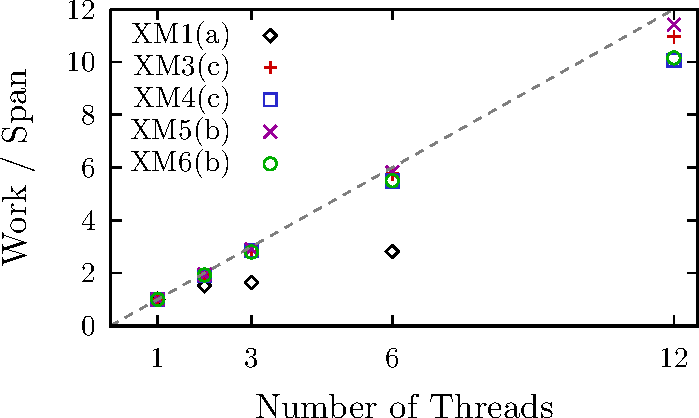
\includegraphics[width=.98\linewidth]{basex/exp_results/load_balance.pdf}
  \caption{Load balance}
  \label{fig:load-balance}
 \end{minipage}
 \hfill
 \begin{minipage}{.48\linewidth}
  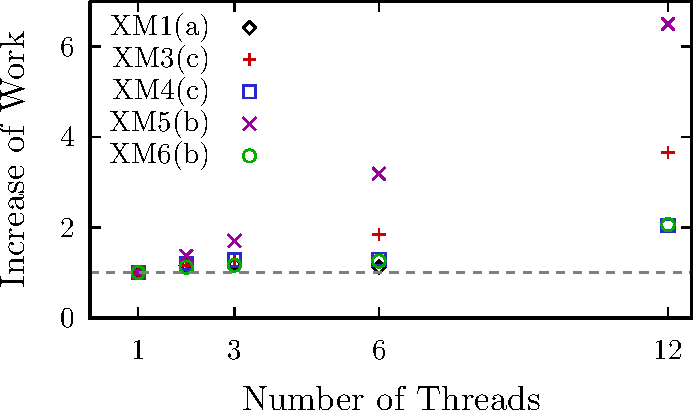
\includegraphics[width=.98\linewidth]{basex/exp_results/increase_of_work.pdf}
  \caption{Increase of work}
  \label{fig:increase-of-work}
 \end{minipage}
\end{figure}

% --------------------------------------------------
\subsection{Evaluation on Implementation of Query Partitioning Strategy}
\label{sec:qpseval}

Table~\ref{tab:qpstotaltime} summarizes the total execution time of the queries.
The ``orig \t{o}'' column shows the time for executing original queries XM1--XM6
and DBLP1--DBLP2 with BaseX's \texttt{xquery} command. The ``seq \t{s}'' columns
show the time for executing all the subquery one by one with a single thread.
The ``par \t{p}'' columns show  the time for executing the x query with one
thread and the with 12 or 6 threads depending on queries. The table also
includes reference of the speedup of parallel queries with respect to original
queries and the size of results of the original queries.


\begin{table}[t]
\centering
\caption{Summary of total execution times(ms) of queries by query partitioning}
\label{tab:qpstotaltime}
	\begin{tabular}{c|c|c|c|c|c}
		\hline
		\multirow{2}{*}{Key} & \multirow{2}{*}{orig \t{o}}  & \multicolumn{3}{c|}{Implementation of Query Partitioning} & Result size             \\ \cline{3-6}
		&                           & seq \t{s}             & par \t{p}             & \t{o}/\t{p}          & Final                   \\ \hline
		XM1(d)               & \multirow{2}{*}{25796.64} & 25326.472           & 11624.09           & 2.22           & \multirow{2}{*}{994M}   \\ \cline{1-1} \cline{3-5}
		XM1(e)               &                           & 31561.45            & 11514.87           & 2.24           &                         \\ \hline
		XM2(d)               & \multirow{2}{*}{1.33}     & 362.564             & 415.38             & 0.00           & \multirow{2}{*}{1.55 K} \\ \cline{1-1} \cline{3-5}
		XM2(e)               &                           & 4.05                & 1.26               & 1.06           &                         \\ \hline
		XM3(d)               & 595.75                    & 754.439             & 146.64             & 4.06           & 14.5 M                  \\ \hline
		XM4(d)               & \multirow{2}{*}{798.16}   & 1098.432            & 516.98             & 1.54           & \multirow{2}{*}{26.4 M} \\ \cline{1-1} \cline{3-5}
		XM4(e)               &                           & 1163.919            & 523.62             & 1.52           &                         \\ \hline
		XM5(d)               & \multirow{2}{*}{659.76}   & 869.089             & 288.21             & 2.29           & \multirow{2}{*}{15.9 M} \\ \cline{1-1} \cline{3-5}
		XM5(e)               &                           & 1536.161            & 1031.46            & 0.64           &                         \\ \hline
		XM6(d)               & \multirow{2}{*}{790.99}   & 744.873             & 646.67             & 1.22           & \multirow{2}{*}{22.2 M} \\ \cline{1-1} \cline{3-5}
		XM6(e)               &                           & 739.449             & 640.57             & 1.23           &                         \\ \hline
		DBLP1                & 3797.36                   & 6572.87             & 1618.51            & 2.35           & 133 M                   \\ \hline
    DBLP2                & 9684.71                   & 12524.70            & 6160.54            & 1.57           & 356 M                   \\ \hline
	\end{tabular}
    \vspace{10px}
	\centering
\caption{Breakdown of execution time (ms)}
\label{tab:qpsbreakdown}
\begin{tabular}{c|c|c|c|c|c|c|c}
	\hline
	\multirow{2}{*}{Key} & \multicolumn{6}{c|}{Subqueries}                              & \multirow{2}{*}{Merge} \\ \cline{2-7}
	& P=1      & P=2      & P=3      & P=6      & P=12    & t$^1$/t$^{12}$ &                        \\ \hline
	XM1(d)               & 25606.42 & 18583.66 & 18701.76 & 11420.36 &         & 2.24   & 203.73                 \\ \hline
	XM2(d)               & 356.67   & 384.08   & 367.99   & 345.89   & 415.38  & 0.86   & 0.00                   \\ \hline
	XM3(d)               & 540.14   & 327.03   & 241.33   & 159.63   & 141.82  & 3.81   & 4.82                   \\ \hline
	XM4(d)               & 897.38   & 786.46   & 550.56   & 507.15   &         & 1.77   & 9.83                   \\ \hline
	XM5(d)               & 670.15   & 415.35   & 314.01   & 284.40   & 282.14  & 2.38   & 6.07                   \\ \hline
	XM5(e)               & 701.94   & 698.77   & 735.18   & 828.65   & 1025.09 & 0.68   & 6.37                   \\ \hline
	XM6(d)               & 789.65   & 799.93   & 790.82   & 636.41   &         & 1.24   & 10.26                  \\ \hline
	DBLP1(d)             & 4035.83  & 2609.61  & 1931.22  & 1567.33  & 1584.97 & 2.55   & 33.53                  \\ \hline
\end{tabular}
\end{table}


\subsubsection{Total Execution Times and Speedups}

From Table~\ref{tab:qpstotaltime}, we can see that for most of the queries we
have obtained speedups of factors  more than 1 and XM3(d) obtains the most
speedup of a factor of 4.06. This means that we can accelerate the execution by
query partitioning for these queries. We also notice that there are two queries,
on the contrary, which have been decelerated: XM2(d) and XM5(e), even with up to
12 threads.

Now, we explain the causes of the slowdown of the two queries.

For XM2(d), one obvious reason is that the original query takes too short time
(only 1.33 ms), while the partitioned  subqueries take extra time for parallel
execution and merge operation. However, there still a big gap between XM2(d) and
XM2(e), i.e. XM2(e) takes quite less time than XM2(d) and is much close to the
original query of XM2. The difference is caused by the subqueries. For XM2(d),
since XM2 is partitioned by the \texttt{position} function at the position right
after \texttt{/site/regions/*}, it evaluates all the nodes that matches queries,
thus taking over 500 ms to complete the query. While for XM2(e), it actually
uses the attribute optimization so that the execution time has been greatly
reduced. This is because the subqueries of XM2(e) have complete paths. For
example, one of its subquery is
\texttt{/site/regions/africa/item/../parent::item/@id}. Since the full path is
contained in the subquires, BaseX can use \texttt{db:attribute("xmark10",
"category52")} to visit only the attribute nodes with the name ``\texttt{category52}'',
avoiding all redundant evaluations over nodes that are not of that attribute
name and thus achieving good optimization on execution time.

As for XM5(e), the partitioning point is just after the step of \texttt{bidder},
of which there are 597797 children nodes. For example, the first subquery of
XM5(e) is\\ \verb|/site/../bidder[position()= 1 to 49816]/increase|, letting P =
12. Note that the number of nodes that matches
\verb|/site/open_auctions/open_auction| is not 1 but 120000. In this case,
when BaseX evaluates the first subquery,  it actually traverses all 12000
\texttt{open\_auction} nodes and evaluates the first 69816 child nodes
\texttt{bidder} of each \texttt{open\_auction}. We investigate the number of
children of \texttt{open\_auction} and the max number is only 62. This means
that only the first subquery can retrieve resultant nodes, while the rest nodes
simply obtain nothing. From this result, we observe that to utilize
position-based query partitioning strategy, we need to guarantee the query before the
point where partition occurs should be a single path, i.e. the number of nodes that match
the query should be one.




\subsubsection{Breakdown of Execution Time}

In this section, we investigate execution times in greater details by analysing
the breakdown of execution time. All the settings are the same as that of data
partitioning.

We first observe that for most queries we can reduce execution time by adding
more threads. For example, XM1(d), XM3(d), XM4(d) and XM5(d) can be apparently
accelerated. While for XM2(d), and XM5(e), the execution times are actually
increased. Besides the reason given in the previous section, there is another
reason introduced in Section~\ref{sec:dpsscal} that the parallelization also
brings overhead compared to the original query and it increases with respect to
the number of threads increased. We also notice that XM6(d) is improved rather
small. This is because the imbalance of the input XML document
\texttt{xmark10.xml},  i.e. the six children of the root contain quite different
amount of descendant nodes,  thus making the reduction of execution time by
adding threads not very obvious.


\section{Observations and Perspectives}
\label{sect:concl}

In this paper, we have revived data partitioning \cite{BoLS09}
on top of BaseX and experimentally demonstrated, in the best case of non-trivial
queries, 4-fold speedup on a 12-core server. In this section, as
concluding remarks, we discuss possible improvement of BaseX in terms of 
partitioning strategies and further perspectives on BaseX.


\subsection{BaseX Extensions Desirable}

Since the implementations of query partitioning is reletively simple and mainly
influenced by the structure of input XML documents as we observed, we mainly
focus on the implementations of data partitioning strategies in this discussion.

Although the client-side implementation generally fell behind the server-side
one in our experiments, it has an advantage that it requires less functionality
of XML database servers. If that performance gap were filled, the client-side
one would be preferable. Since the performance gaps in prefix queries were small
even when their result sizes were more than 1 MB, the difference of cost between
sending prefix results to (local) clients and storing them in a server was
marginal. The dominant factor was the cost of sending prefix results back in the
form of long suffix queries and parsing them on a server.  A promising approach
to reducing this overhead is client-server streaming of the starting nodes of a
suffix query. Since one suffix query is in common applied to many starting
nodes, if the suffix query is given to a server in advance, the server can apply
it successively to incoming starting nodes and stream out results to clients.
With this streaming functionality additionally, the client-side implementation
would perform fast nearly to the server-side one.

There is also room for improvement of the server-side implementation. We store
block-partitioned arrays into an in-memory database as text parts and then
deserialize them to sequences. This is, to the best of our knowledge, the most
efficient way of preserving arrays on top of the current BaseX server, but is
merely a workaround because its serialization/deserialization is redundant. The
most efficient way is obviously to keep XQuery data structures as they are on
top of a server. We consider that it would not necessitate a drastic change of
BaseX. Only demand-driven serialization and new function \Src{deserialize}
suffice for it as follows. When XQuery values are put into a text part of an
in-memory database, they are not serialized immediately but keep their
representations. They will be serialized for a query just before the query tries
to read the text part. If a query applies \Src{deserialize} to the text part, it
returns their original representations in zero cost. It is worth noting that
because in-memory databases in BaseX will never be stored on disks,
demand-driven serialization per se is worth implementing to avoid serialization
into text parts not to be accessed.

\subsection{Further Perspectives}

Both data partitioning and index-based optimizations have worked together well
only with the simple way described in Section~\ref{sect:opt}. Both lie in the
same spectrum in the sense that performance gain is contingent on the statistics
of a given document. In fact, document statistics are known to be useful for
data partitioning (as well as query partitioning)
\cite{Bord10}. Statistics maintained together with indices
in BaseX should therefore be utilized for data partitioning together with
index-based optimizations. If we implement data partitioning into BaseX, a close
integration with both would be naturally feasible. Besides, statistics will be
available even outside BaseX by using \emph{probing} queries that count nodes
hitting at a specific step. The cost of several probing queries in advance to
data partitioning would matter little because simple counting queries are quite
fast on BaseX.  By using node counts, we can avoid the situation of an
insufficient number of prefix query results found in XM1(a). It will be a
lightweight choice in the sense of preserving a black-box use of BaseX.

It is challenging yet promising to extend data partitioning to distributed
databases with BaseX. The top part of a document to be traversed by prefix
queries can be either centralized or replicated. Bottom parts to be traversed by
suffix queries should be distributed as separate XML databases. Because the
whole database forms a simple collection of XML documents, horizontal
fragmentation \cite{kling11:dist_xml} will be well-suited but it can incur
imbalance in size among fragments. Balanced-size cheap fragmentation based on
partial trees \cite{HaMa16} will be promising for the complement to it. Existing
work \cite{DaGK14} on querying large integrated data will be relevant. Hybrid
partitioning \cite{BoLS09}, which is combination of data partitioning and query
partitioning, would become important because query partitioning requires
synchronization only in merging partial results and the number of
synchronizations matters more in distributed databases. Fragmentation-aware
hybrid partitioning is worth investigating. The most challenging part is to
implement integration with existing index-based optimizations so as to take
account of global information, where our idea described in
Section~\ref{sect:opt} will be useful but would not be trivially applicable.

\section{Summary}

First, as concluded in~\cite{BoLS09}, it is not obvious if data or query
partitioning would be beneficial. In our implementations, these are caused by
different factors. For the implementations of data partitioning, we need to
process a prefix query before processing the suffix queries in parallel. This is
a extra cost compared to the original query and the amout of extra time for
processing a prefix query relates to the result size of the prefix query. In
case the result size is large, it takes a lot time, such as DBLP1(a) and
DBLP2(a). While for the implementations of query parititioning, the imbalance of
XML documents have a dramatic influence on the query perfomrance and the
speedup.

Second, BaseX optimizer plays an important role in the reduction of execution
time. In case when BaseX optimizer is available, execution time can be greately
reduced. A very important feature of the optimizer is that it can also be
applied in parallel evaluation. Therefore, it is worth taking the optimizations
to reduce the execute time as long as the partition of subqueries can meet the
conditions of the BaseX optimizer.

Third, the experiment results clearly show that we can achrive speedup up to 4,
which have strongly proved that the partitioning stragegies are available not
only on XML trees but also on XML database engines. However, the availability of
these stragegies is significantly dependent on the implementations and the XML
database engine/processor. Properly combined with the features of the XML
database engine/processor used for implementation, we can achrive significant
performance improvements over the original strategies, such as the server-side
implementation of data partitioning strategy.



\section{Introduction}

Data partitioning strategy was originally studied in a shared-memory
environment, where XML data is stored in a shared memory and can be concurrently
accessible by multiple XPath processors. In the conclusion of the original
paper~\cite{BoLS09},  the authors had pointed out that the parallelization model is over XML
data model, and it can also be adapted to any XML storage laryout. However, no matter in
the original study, or in our previous study, the strategies are applied both
in a shared-memory environment. Therefore, here comes a question:  how we can
apply it in a distributed-memory environment? In this study, by exploiting
horizontal fragmentation on XML data, we present our study on applying data
partitioning in a distributed-memory environment to experimentally show how it
improves the scalability.

\section{Fragmentation}

\subsection{Introduction}
Fragmentation is an effective way to improve scalability of database
systems~\cite{navathe1995mixed, hauglid2010dyfram, khan2010new}.  In the field
of parallel XML processing, there are also some studies on  fragmentation of XML
data~\cite{kling11:dist_xml, KlOD10}.  The most common XML fragmentations are
horizontal fragmentation and vertical fragmentation~\cite{kling11:dist_xml}. Due
to the nature of horizontal fragments that are  relatively independent, it is a
more direct and practical way to work together with data partitioning. We thus
focus on only horizontal fragmentation in this study.

\subsection{Definitions}
We first define horizontal fragmentation.  Let $D$ = \{$d_1$, $d_2$, ...,
$d_n$\} be a collection of document trees such that each $d_i \in D$ conforms
the same XML schema~\cite{xmlschema}.  Let $\mathit{FS}$ = \{$F_1$, $F_2$,...,
$F_m$\}  be a collection of fragments such that for each $F_i \subset D$. If
$\bigcup\limits_{i=1}^{m} F_{i} = F$ and $\bigcap\limits_{i=1}^{m} F_{i} =
\emptyset$, then $\mathit{FS}$ is a horizontal fragmentation of $D$.

Let us take the tree in Fig.~\ref{fig:hfrag_example} as an example. There are
five document trees in Fig.~\ref{fig:hfrag_example}(a), i.e. we have $D$ =
\{$d_1$, $d_2$, $d_3$, $d_4$, $d_5$\}, where $d_1$ is  the first subtree rooted
at $b$ (from left to right), $d_2$ be the second and so on. All the subtrees
follow the schema in Fig.~\ref{fig:hfrag_example}(b). We can make three
horizontal fragments $FS$ = \{$F_1$, $F_2$, $F_3$\} as shown in the three dotted
rectangles, where $F_1$ = \{$d_1$, $d_2$\}, $F_2$ = \{$d_3$\} and  $F_3$ =
\{$d_4$, $d_5$\}.


\begin{figure}[t]
	\centering
	\begin{subfigure}{.6\textwidth}
		\centering
		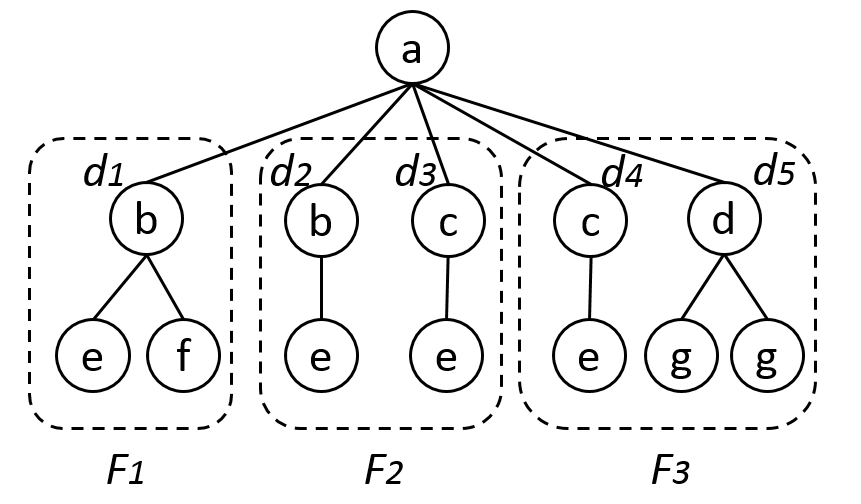
\includegraphics[width=.99\linewidth]{figures/hfrag_example}
		\caption{An example of horizontal fragmentation}
		\label{fig:sub1}
	\end{subfigure}%
	\begin{subfigure}{.4\textwidth}
		\centering
		\vspace{12mm}
		\begin{tabular}{|l|}
			\hline
			schema\\
			\hline
			a(b*, c*, d) \\
			b(e, f?) \\
			c(e) \\
			d(g*) \\
			\hline
		\end{tabular}
		\vspace{12mm}
		\caption{The schema of the example}
		\label{fig:sub2}
	\end{subfigure}
	\caption{An example of horizontal fragmentation and the schema.}
	\label{fig:hfrag_example}
\end{figure}

\subsection{Applying Fragmentation}

In our study, we first apply horizontal fragmentation to the input XML data,
through which an XML tree is divided into a set of fragments. To make the 
fragmentation works well in combination with data partitioning strategy. We
have the following requirements.

\subsubsection{Fragments are size-balanced}

Since the mainpurpose of fragmentation is to achieve good scalability, we
attempt to make our fragmentation algorithm size-balanced, i.e. to make each
fragment have nearly the same amount of node. 

\subsubsection{Path to the root is added}

In our design desire of fragmentation algorithm, we also intent to ease the
querying. Thus, we require that each fragment is a set of consecutive
sibling subtrees augmented with the path to the root. Note that two
subtrees are sibling subtrees if the roots of the subtrees are siblings of each
other.

\subsubsection{Correctness}

We assume that all the results lie in the subtrees on the fragment. Thus,
to guarantee the correctness of query results, we need to guarantee the
completeness and uniqueness of nodes such that each node in the input XML tree
is included in at least a fragment. If a node is included a subtree part of a
fragment, then it is not included in any other fragment.


\begin{figure}[]
	\centering
	\begin{tabular}{l}
		\hline
		\hline
		\makebox[.95\linewidth][l]{\textbf{Algorithm 1} \textsc{Fragmentation}($\mathit{nodes}$, $\mathit{MAXSIZE}$)} \\
		\hline
		\textbf{Input}:           $\mathit{nodes}$: a list of nodes, \\
		\makebox[1em][r]{}\hspace{9 mm}  $\mathit{MAXSIZE} $ : the maximum number of nodes in a fragment \\
		\textbf{Output}: a list of fragments \\
		\makebox[1em][r]{1:}\hspace{1 mm}  $\mathit{fragments} \leftarrow [] $     //a list of fragments \\
		\makebox[1em][r]{2:}\hspace{1 mm}  $subtrees \leftarrow [] $     //a list of root nodes of subtrees \\
		\makebox[1em][r]{3:}\hspace{1 mm}  \textbf{for all} $\emph{node} \in \emph{nodes}$ \textbf{do} \\
		\makebox[1em][r]{4:}\hspace{5 mm}  \textbf{if} \texttt{size($node$)} $ > \mathit{MAXSIZE} $ \textbf{then} \\
		\makebox[1em][r]{5:}\hspace{9 mm}  \textbf{if} $subtrees.length > 0$  \textbf{then} \\
		\makebox[1em][r]{6:}\hspace{13 mm} $\mathit{fragments}.Add((\textit{\_, subtrees}))$ \\
		\makebox[1em][r]{7:}\hspace{13 mm}  $\mathit{subtrees} \leftarrow []$ \\
		\makebox[1em][r]{8:}\hspace{9 mm}  \textbf{end if}\\
		\makebox[1em][r]{9:}\hspace{9 mm}  $\mathit{fragments}.AddAll($\texttt{Fragmentation}$($\texttt{child}$(node), \mathit{MAXSIZE}))$ \\
		\makebox[1em][r]{10:}\hspace{5 mm}  \textbf{else if} \texttt{size($node$)} + \texttt{Size}$(subtrees) > \mathit{MAXSIZE}$ \textbf{then} \\
		\makebox[1em][r]{11:}\hspace{9 mm} $\mathit{fragments}.Add((\_, subtrees))$ \\
		\makebox[1em][r]{12:}\hspace{9 mm} $subtrees \leftarrow [node]$ \\
		\makebox[1em][r]{13:}\hspace{5 mm}  \textbf{else}\\
		\makebox[1em][r]{14:}\hspace{9 mm} $\mathit{subtrees}.Add(node)$ \\
		\makebox[1em][r]{15:}\hspace{5 mm}  \textbf{end if}\\
		\makebox[1em][r]{16:}\hspace{1 mm}  \textbf{end for}\\
		\makebox[1em][r]{17:}\hspace{1 mm}  \textbf{for} $i \in [0, \mathit{fragments}.length)$ \textbf{do}\\
		\makebox[1em][r]{18:}\hspace{5 mm}  $\mathit{fragments}[i] \leftarrow $\texttt{AddPath}($\mathit{fragments}[i]$)  \\
		\makebox[1em][r]{19:}\hspace{1 mm}  \textbf{end for}\\
		\makebox[1em][r]{20:}\hspace{1 mm}  \textbf{return} $\mathit{fragments}$\\
		\hline
	\end{tabular}
	\caption{The fragmentation algorithm.}
	\label{fig:algQuery1}
\end{figure}


\begin{figure}[]
	\centering
	\begin{tabular}{l}
		\hline
		\hline
		\makebox[.95\linewidth][l]{\textbf{Algorithm 2} \textsc{AddPath}($\mathit{subtrees}$)} \\
		\hline
		\textbf{Input}:   $\mathit{subtrees}$: a list of root nodes of subtrees \\
		\textbf{Output}:  the root node of a tree that is augmented with the \\
		\makebox[1em][r]{}\hspace{13 mm}  path to the root of the whole tree\\
		\makebox[1em][r]{1:}\hspace{1 mm}  $\mathit{p} \leftarrow $\texttt{parent}$(subtrees[0]) $   \\
		\makebox[1em][r]{2:}\hspace{1 mm}  $node \leftarrow $ \texttt{clone}($p$)    \\
		\makebox[1em][r]{3:}\hspace{1 mm}  $node.addChildren(subtrees) $ \\
		\makebox[1em][r]{4:}\hspace{1 mm}  \textbf{while} \texttt{parent}$(p) \neq \mathit{NULL}$ \textbf{do}\\
		\makebox[1em][r]{5:}\hspace{5 mm}  $p \leftarrow $ \texttt{parent}($p$) \\
		\makebox[1em][r]{6:}\hspace{5 mm}  $tempnode \leftarrow$ \texttt{clone}($p$)  \\
		\makebox[1em][r]{7:}\hspace{5 mm}  $tempnode.addChild(node)$ \\
		\makebox[1em][r]{8:}\hspace{5 mm}  $node \leftarrow tempnode$ \\
		\makebox[1em][r]{9:}\hspace{1 mm}  \textbf{end while} \\
		\makebox[1em][r]{10:}\hspace{1 mm}  \textbf{return} $\mathit{node}$\\
		\hline
	\end{tabular}
	\caption{Add path to a list of subtrees}
	\label{fig:algQuery2}
\end{figure}

\begin{figure}[!t] 
	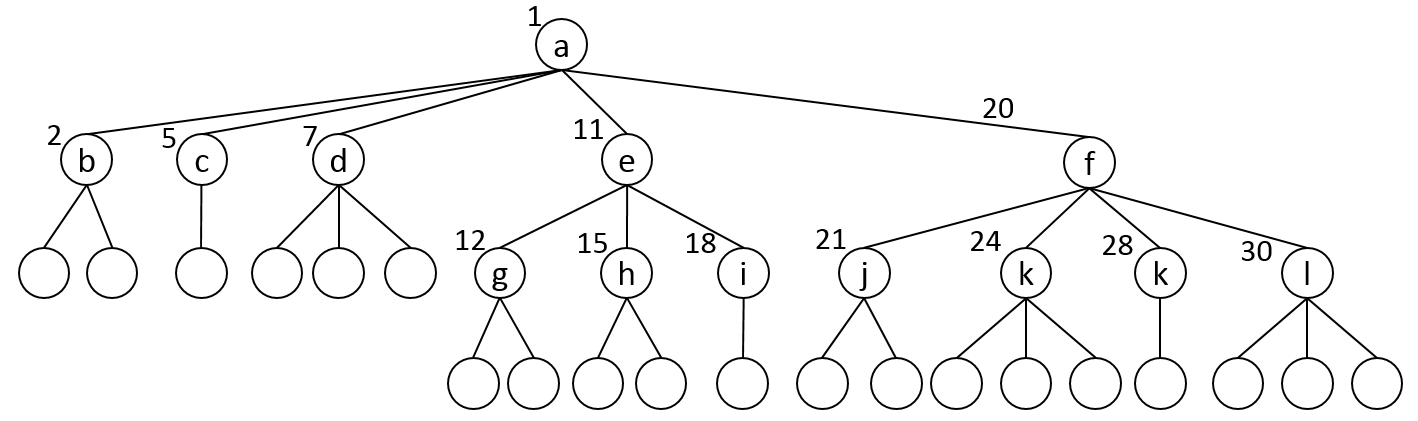
\includegraphics[scale=0.38]{figures/fragment1}
	\caption{An example tree with number denoting PRE values of nodes}
	\label{fig:frag1}
	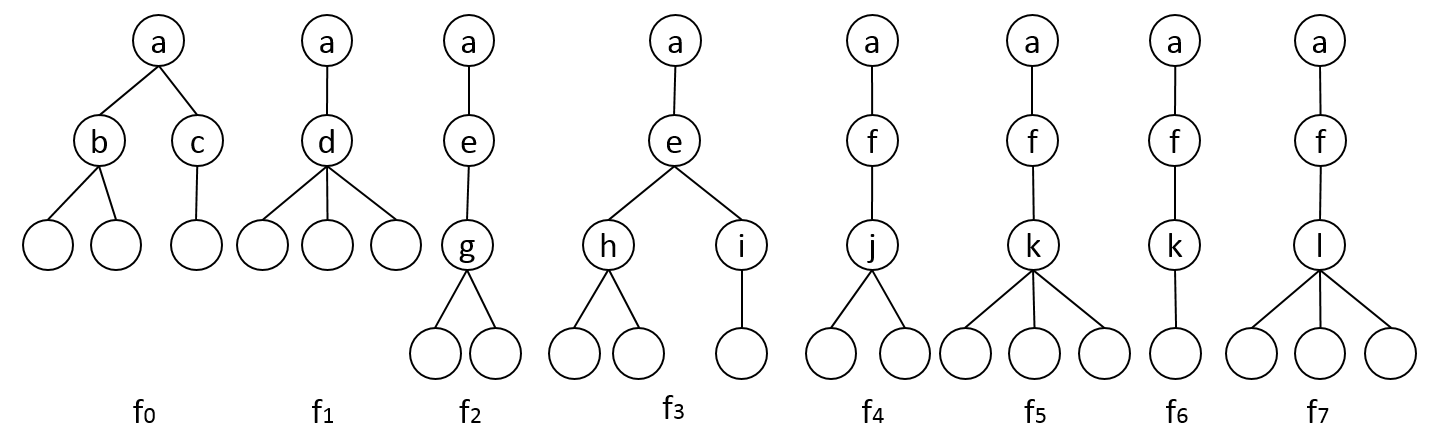
\includegraphics[scale=0.38]{figures/fragment2}
	\caption{Recontructed fragments.}
	\label{fig:frag2}
	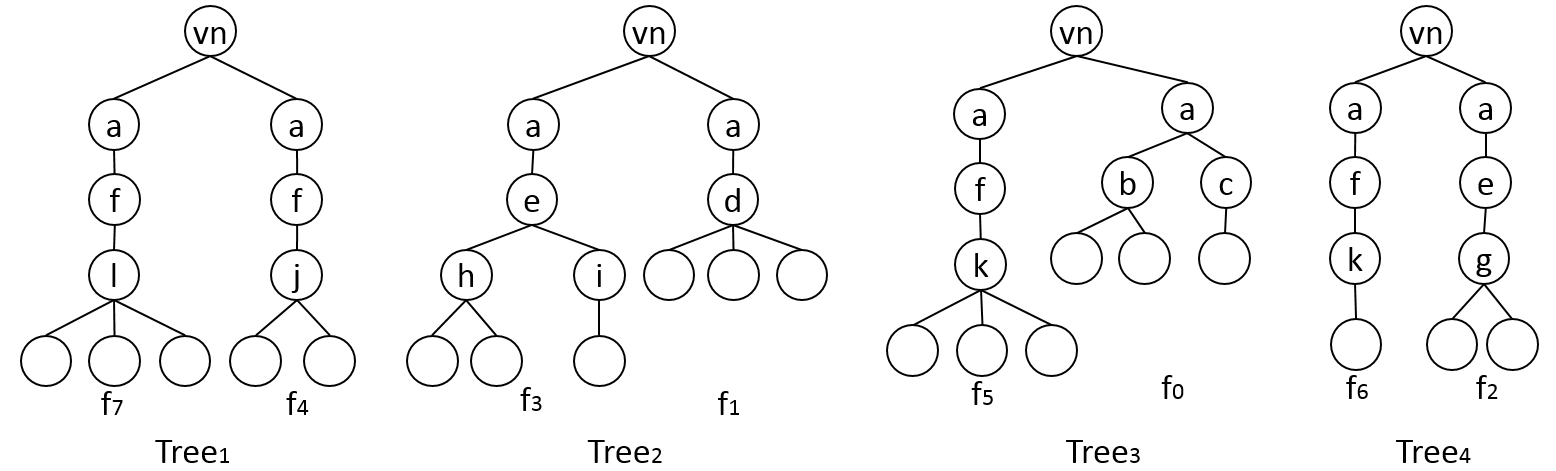
\includegraphics[scale=0.35]{figures/fragment3}
	\caption{Regroup and merge.}
	\label{fig:frag3}
\end{figure}



Algorithm 1 describes how our fragmentation works to apply a horizontal
fragmentation to a tree. The arguments of input are a list of nodes denoting the
tree to be fragmented and an integer number denoting the maximum number of nodes
a fragment can have so that we can make the fragments in similar size.   In Line
1--2, we declare an empty list of fragments and an empty list of subtrees for
holding results. In Line 3--16, we traverse each node in the input list, if the
node have more number of descendant nodes greater than MAXSIZE, we apply the
fragmentation on the children of the node (Line 4--9) and add the results into
$fragments$. Else if total number of descendant nodes in $subtrees$ and the
$node$ excesses MAXSIZE, we save the current fragment and put the current node
into a new fragment (Line 10--12). Otherwise, the current node is added to
$subtrees$ as one of the subtrees in the current fragment. After the iteration,
we obtain a list of fragments, each of which is a list of subtrees. We add the
last use Algorithms 2 to complete each fragment by adding the path from the
current subtrees to the root of the original tree (Line 17--19). In Algorithm 2,
we basically keep looking upward, to add all the ancestor nodes to the current
fragment.

There are also several functions used in Algorithms 1 and 2 that are described 
as below:\\
- \texttt{size($node$)} returns the number of descendants of $node$, where node
is a single node.\\
- \texttt{Size($nodes$)} returns the sum of number of descendants of each node
in $nodes$, where $nodes$ is a list of nodes.\\
- \texttt{child($node$)} returns the children of $node$.
- \texttt{parent($node$)} returns the parent of $node$.\\
- \texttt{clone($node$)} returns a node cloned from $node$. The function create
an empty node and copy the name and attributes from $node$.

Note that for the query processing, we need a representative value for each
fragment to maintain the original order of a fragment as in the original tree.
We simply use a fragment id for each fragment.

Let us take the tree shown in Fig.~\ref{fig:frag1} as an example with MAXSIZE =
3. After Line 16 of Algorithm 1, the fragments are list of subtrees. When we use
the PRE index to denote the root node of a subtree, we have F = [f$_1$, f$_2$, ...,
f$_8$] = [[2, 5], [7], [12], [15, 18], [21], [24], [28], [30]], where the
subscripted numbers are the fragment ids. Then, by applying Algorithm 2 that adds
the path from the subtrees to the root of the whole tree, we obtain the final
recontructed fragment as shown in Fig.~\ref{fig:frag2}.

\section{Our Ditributed XPath Query Framework}

We design an XPath query framework using horizontal fragmentation with data
partitioning strategy on top of BaseX over a distributed-memory environment. 
In this framework, there are one client and $N_s$ servers. The client is a
computer running a Java program that is the implementation of our query
algorithm. It works for sending queries to multiple servers and processing
results returned from them. A server is a computer that runs a BaseX server in
charge of evaluating received queries. An input dataset will be fragmented and
distributed to all the servers to be queried and the results returned from all
the servers will be merged on the client.

It consists of the following four stages:\\
\begin{itemize}
	\item Data Fragmentation \\To divide an input XML document into fragments.
	\item Allocation\\ To assign the fragments into multiple computation nodes.
	\item Query Evaluation\\ To query fragments in parallel
	\item Results Merging\\ To merge the results of fragents to form the final result.
\end{itemize}



We give the detailed introduction in the following sections.



\subsection{Allocation}

After fragmentation, the fragments are mapped to multiple computation nodes. For each
computation node, a sub set of fragments is assigned. To make the distribution
of fragments well-balanced, we randomly shuffle the list of fragments before
dividing the list into $N$ lists of fragments, where N is the same as the number
of computation nodes. 

We use a mapping list to map the fragments. An element in the mapping list
contains information for locating the corresponding fragment so that we can
access and process query on the fragment independently.  With this mapping list,
we can start a query by locating the root of each fragment on any tree, making
it possible to evaluate queries on them in parallel.  And also, the mapping list
can be used to maintain the order of results to form the final results.

In our study, we run a single BaseX instance in server mode on each computation
node. For each computation node, the sub set of fragments on it is then added to
an empty root node to form a complete XML tree so that we can load the tree by
the BaseX server to create an XML database for further query evaluation. To make
each list of fragments become a single tree (so that we can create a database in
BaseX from it),  we create a node as the root and add the lists of the fragments
to the root, where the root of a fragment becomes the child of the newly added
root node. 

Let us continue the running example. Let N be 4, after shuffling and regrouping,
we may obtain four groups of fragments: FS $=>$ [F$_1$, F$_2$, F$_3$, F$_4$], where
F$_1$ = [$f_7$, $f_4$],
F$_2$ = [$f_3$, $f_1$],
F$_3$ = [$f_5$, $f_0$],
F$_4$ = [$f_6$, $f_2$].
By adding a root node $vn$ to the each group, we create four trees from FS
respectively as shown in Fig.~\ref{fig:frag3}.

We also create a mapping list of links $links$ for each F in FS for locating.
A link is a 3-tuple ($Tree,
pre, depth$), where $tree$ is a pointer to a reconstructed tree, $pre$ is the PRE
value of the root of a fragment in $tree$, $depth$ is the number of nodes in the
path from subtrees to the root. For the given example, we have a list of links
$links$ =
[(Tree$_3$, 2, 1),
(Tree$_2$, 9, 1),
(Tree$_4$, 6, 2),
(Tree$_2$, 2, 2),
(Tree$_1$, 8, 2),
(Tree$_3$, 2, 2),
(Tree$_4$, 2, 2),
(Tree$_1$, 2, 2)],
where $links[0] \rightarrow f_0$, $links[1] \rightarrow f_1$, ...,  $links[7]
\rightarrow f_7$.

\section{Query evaluation}

\subsection{Rewriting An XPath Query In XQuery}

An input XPath query is rewritten into an XQuery expression to be then processed
by BaseX servers. The rewriting is different depending on whether data
partitioning strategy is used or not.

\subsection{Without Data Partitioninng Strategy}
\label{no-dps}

Since the nodes in the results will no long follow the original order in the
input document, we return the nodes along with their PRE index for later
identifying and reordering by using the following expression.

\verb|for $node in db:open(`db')$query|\\
\verb|     return ((`', db:node-pre($node)), $node)|
\footnote{\texttt{return (a, b)} will add a line break between \texttt{a} and
	\texttt{b} while returning.}

We separate the PRE value and the content of a node by a linebreak and add an
extra linebreak among resultant nodes\footnote{According to my previous
	implementation and tests, it worked.}.


\subsection{With Data Partitioning Strategy}

When applying data Partitioning, we use the server-side implementation. In
order to maintain the order of resultant nodes, we make some change to the
server-side implementation. For the two-phases implementation, we do not need to
change the first phase, which still returns the PRE values of the results of
prefix query. We need to change the second phase, where the \verb|return|
statement in the suffix query needs to be modified to 
\verb|return ((`',db:node-pre($node)), $node)|, 
i.e. the same as the XQuery expression described in~\ref{no-dps}.

 

\section{Evaluating Queries}

The evaluation an XPath queries consists of two steps: sending query and
processing results.

\subsection{Sending query}

After an input query being rewritten, it will be sent form the client to all
srevers for executing. After sending, the client will be idle waiting for
results to be sent back.

\subsection{Processing Results}

The results are returned from all servers through the network (some servers may
return empty results). There are two issues we need to consider when processing
results. First, since the size of results can be larger than the memory size of
the client (such as XM1 that returns about 90 the size of the input data), we
thus store results on disk. Second, due to the randomization, the results
returned from all servers are not in the original order. Thus, we have to
recover the original order of results when processing. It is different to deal
with the order depending on whether data partitioninng strategy is used.

\subsection{Without Data Partitioning Strategy}

First, since we have the PRE values of resultant nodes, we can use them to
determine which fragment a resultant node belongs to by comparing with the
$mpre$ of each fragment, where $mpre$ is the PRE value of the root of the first
subtree in the fragment. Given a list of fragments $F$ = \{$f_0$, $f_1$,...,
$f_n$\}, a function \textsc{GetMpre($f$)} that returns the $mpre$ of the
fragment $f$ and the PRE value $pre$ of a node $n$, if \textsc{GetMpre($f_i$)}
$\leq pre <$ \textsc{GetMpre($f_{i+1}$)}, ($i  < n$ - 1) or
\textsc{GetMpre($f_i$)}$\leq pre$, ($i = n$ - 1), then $n$ belongs to $f_i$. For
example, there are three fragments, and their $mpre$ are 3, 10, 20 respectively.
A node with the PRE value 5 belongs to the first fragment. Note that we do not
need to deal with the order of the nodes in the same fragment, because these
nodes in the same fragment still keep the original order. Thus, the results can
be grouped by fragments.

Next, we store the results in a list of files, each of which stores the results
that belong to the same fragment. We use fragment id to name these files so
that we can obtain the results stored in these files in the original order, when
reading the files ordered by their names

Through the above method, since all the fragment can be processed separately, we
can receive the results and save them to disk in parallel.

\subsection{With Data Partitioninng Strategy}

Since data partitioninng strategy uses multiple processors, results of the same
fragment may be processed by two processors. For example, when we use two
processes $p_1$ and $p_2$ to process the same merged tree with only one fragment
$f_0$, the resultant nodes in the fragment may be processed by both processors.
Since there is only one file that corresponds the fragment for storing, the two
processor cannot write the resutls to the file at the same time.

There are two ways to solve the problem. One way is to write the results in
sequential, i.e. we let only one processor to write at a time. For example, we
let $p_1$ write first then $p_2$ follows. However, this way should be slow, because
when a processor is writing results, the following processors have to wait.
Another way is simply to add a suffix to the file names then concatenate files
with suffix. For the above example, $p_0$ changes the file name to
\texttt{0\_start.txt} and $p_1$ to \texttt{0\_end.txt} for the fragment $f_0$.
After receiving all the results, we concatenate the two files to \texttt{0.txt}.
In this way, we can still process the results in parallel. But in some extreme
case when the results of a fragment is very larger, the concatenation may bring
significant overhead.



\section{Experiments}

For the experiment part, I decide to use 4 computers, each has 4 cores
(matsu-lab50--matsu-lab53). The XMark dataset sizes 4.4 GB with 66.65M nodes.
The MAXSIZE is set to 4.2M, so that we can divide the dataset into 16 fragments
(my intention is to assign one to each core). I use two settings for
experiments. One that only runs queries in parallel and the another also applies
to data partitioning strategy. We will compare the two setting to show how much
DPS can be used to improve the query efficiency.







\chapter{Partial Tree}
\label{ch:partialtree}

%\section{Definitions}
\label{sec:partialtree}

In this section, we introduce our novel tree structure, partial tree. Parital
tree  is used to process XPath queries over an XML documents in parallel. To use
partial tree, we first split an XML document into many chunks and then from
these chunks, we can construct multiple partial trees from the chunks. To deeply
understand what partial tree is, we first give some definitions for it.


To begin with, we give the defintion of types of element nodes. A partial
tree contains four different types of element nodes as shown in
Figure~\ref{fig:nodetypes}. The four types of element nodes in the figure are:
\emph{close node},  \emph{left-open node},  \emph{right-open node} and
\emph{pre-node}. A closed node is a regular node that has both its start tag and
end tag. For a node that does not have both of its tags, we call it \emph{open
node}, including left-open node, right-open node and pre-open node. A left-open
node has only its start tag, while a right-open node has only its end tag. In
case a node loses both of its tags, we call it \emph{pre-node}.

Open nodes are not a new concept. Kakehi et al~\cite{KaME07} proposed a new
approach for parallel reductions on trees and explicitly used 'open' nodes in
their paper. Choi et al.~\cite{ChLL14} proposed an idea to label nodes in split
chunks of a large XML documnet. Although they did not use the term, but the idea
is exact the same as that of open nodes.

A pre-open node is a novel idea proposed in our study and is different from the
other two open nodes that it comes from no tag, i.e. we do not create a pre-node
directly from the corresponding tags. This is becuase the corresponding tags of
a pre-node do not exist in the chunk.  This is, on the contrary, the most
significant idea of this study, so that we can use it to represent the missing
nodes on the path from the root of the whole tree to current subtrees parsed
from a chunk, which specifies the relationships between the root of the whole
tree and the substrees.

Note that (1) since our research focuses on evaluating queries on partial trees,
more specifically, mainly on element nodes, in case no tag is contained in a
chunk, we merge it to the next chunk until there is at least a tag existed in
the chunk (this is very rare case only when a context is too large or the chunk
is too small); (2) all open nodes, including pre-node, are element nodes.
Therefore, we omit attribute and content nodes in this section for
simplicity.

% Attribute and context nodes have been introduced in Chapter 3.


For representing open nodes separately from the close nodes in figures, we add
one black dot: $\bullet$ to an open node representing the side on which the node
is open, i.e. which tag is missing. For the example, when we split the pair of
tags \texttt{<A></A>} into two tags, we can create an right-open node A$\bullet$
from \texttt{<A>} and a left-open node $\bullet$A from \texttt{</A>}.


Last, based on the above definitions, we now give the definition to partial
tree. A partial tree is a tree structure with open nodes and represents a chunk
of an XML document and can be used for parallel XML processing.


\begin{figure}[t]
\centering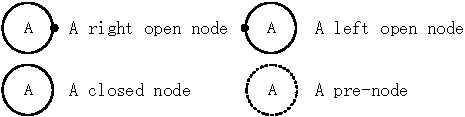
\includegraphics{partialtree/figures/fromWord-2.pdf}
\caption{Four types of element nodes}
\label{fig:nodetypes}
\end{figure}

%
%
\section{Characteristics of Partial Tree}
\label{sec:chars}

Now we discuss the Characteristics of partial trees. Since the left-open nodes,
right-open nodes and pre-nodes are most significant concept in partial trees, we
first focus on the properties of these open node.

\subsection{Properties of Open Nodes}

We introduce three properties of open nodes. The first property is about the
parent-child relationship of the open nodes.

\begin{property}
\label{property1}\itshape
If a node on a partial tree is left/right open, then its parent is also
left/right open.
\end{property}

The second property is about the sibling relationship of the open nodes.

\begin{property}
\label{property2}\itshape
If a node is left open, it is the first node among its
siblings in the partial tree. If a node is right open, it is the last
node among its siblings in the partial tree.
\end{property}

There is another important property of pre-nodes.

\begin{property}
\label{property3}\itshape
If there exist multiple pre-nodes, then only one of
them has left-open/closed/right-open nodes as its child.
\end{property}


\subsection{Standard Structure}

According the properties of partial tree, the standard structure of partial tree
can be described as in Fig.~\ref{fig:model}.

\begin{figure}[t]
\centering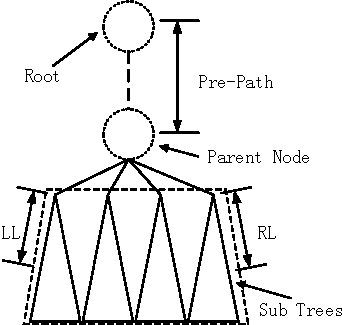
\includegraphics{partialtree/figures/fromWord-4.pdf}
\caption{The standard structure of partial tree.}
\label{fig:model}
\end{figure}

A partial tree consists vertically of two parts. The bottom part is a forest
of subtrees and the top part is a list of pre-open nodes denoting the path from
the root to the bottom part. We call the list of pre-open nodes emph{pre-path}.
Pre-path plays an important role in applying queries from the root. From
property~\ref{property3}, one or more subtrees connect to a pre-node at the
bottom of the pre-path. Note that for each subtree, there is only one root,
which is a left-open/closed/right-open node, but there could be one or more
subtrees.

From properties \ref{property1} and \ref{property2}, we know that left-open
nodes are located on the upper-left part of a partial tree and the right-open
nodes are located on the upper-right part. More precisely, the left-open nodes
form a list from a root node of a subtree, and we call the list the \emph{left
list} (LL). Likewise, we call the list of right-open nodes the \emph{right list}
(RL).

%
%
\def\INDEXSET#1{\mathit{#1}_{[P]}}
\def\baselinestretch{1.5}

\section{Construction of Partial Trees}
\label{sec:construction}

Since the structure of partial tree is quite different from ordinary XML trees,
especially the pre-path, ordinary XML parsing algorithms, in turn, do not work
for the construction of partial tree. The difference mainly lies in two aspects.
First, an XML document can generate only a single XML tree. While in case of
partial tree, the number of XML trees could be many, which is determined by the
number of chunks. However, we cannot simply construct an partial tree from a
chunk. This is caused by the second reason that the pre-path of a partial tree
is missing in the corresponding chunk.

For constructing the pre-path, it is important that a partial tree that
corresponds to a chunk is the minimum subgraph. It should satisfy the following
three conditions:

(1) the subgraph is connected (This means the subgraph is a tree.);

(2) each node in the chunk is in the subgraph, and

(3) the root of the original XML tree is in the subgraph.

For an intuitive grasp, we use the following XML document as the running
example.

\begin{quote}\tt\small
<A><B><C><E></E></C><D></D></B><E></E><B><B><D><E>\\
</E></D><C></C></B><C><E></E></C><D><E></E></D></B>\\
<E><D></D></E><B><D></D><C></C></B><B></B></A>\\
\end{quote}

From the document, we can construct an XML tree as shown in Fig.~\ref{fig:tree}.
We number all the nodes of the tree in a prefix order for identification.



To construct partial trees from the document, we first split it into five chunks
as listed below.

 chunk$_0$: \texttt{ <A><B><C><E></E></C><D></D></B>}

 chunk$_1$: \texttt{ <E></E><B><B><D><E></E></D>}

 chunk$_2$: \texttt{ <C></C></B><C><E></E></C><D>}

 chunk$_3$: \texttt{ <E></E></D></B><E><D></D></E>}

 chunk$_4$: \texttt{ <B><D></D><C></C></B><B></B></A> }


\begin{figure*}[t]
	\centering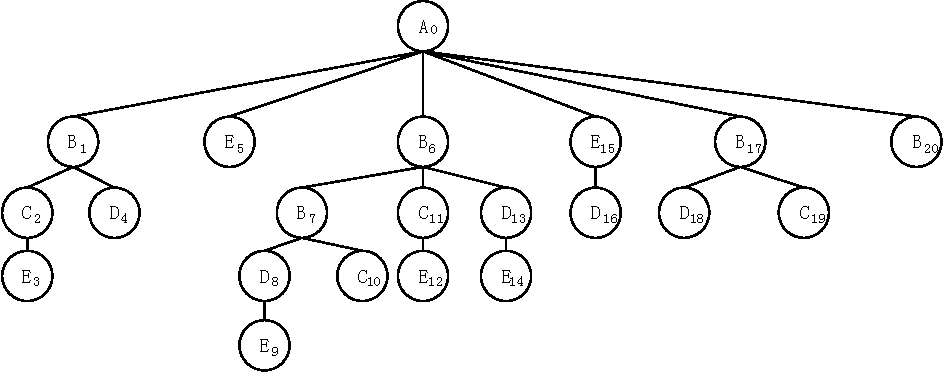
\includegraphics[scale=.9]{partialtree/figures/fromWord-5.pdf}
	\caption{an XML tree from the given XML string}
	\label{fig:tree}
	
	\centering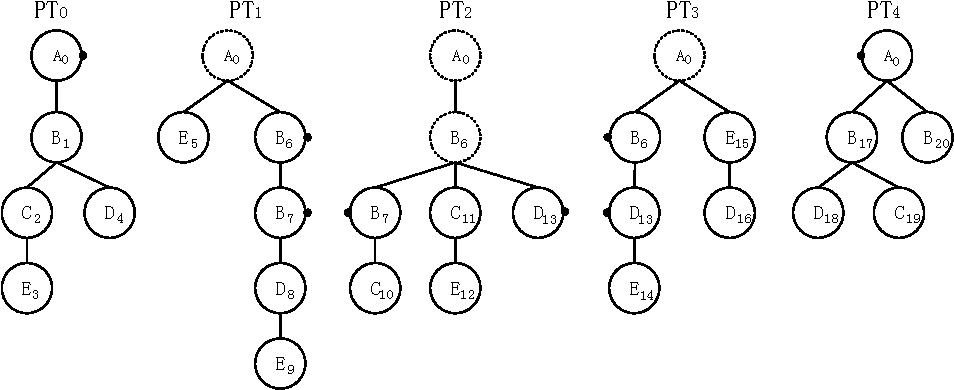
\includegraphics[scale=.9]{partialtree/figures/fromWord-7.pdf}
	\caption{Partial trees from the given XML string.}
	\label{fig:partialtree2}
\end{figure*}

We can construct a parital tree from each chunk, i.e. chunk$_i$ makes a partial
tree PT$_i$, as shown in Figure~\ref{fig:partialtree2}.

In the following section, we introduce our partial tree construction algorithm
with the example. Our algorithm is a three-phase algorithm. In the first phase,
we construct mutiple sets of subtrees that have some open nodes from parsing
chunks of the input XML document. Second, we compute pre-path for each list of
subtrees with all the open nodes. Last, we add pre-paths to the corresponding
list of subtrees to complete the partial tree construction. We will give deailed
introduction to the three-phase construction algorithm of partial tree.
Furthermore, to server the query algorithm, we also introduce the statistics
information of open nodes, called ranges of open nodes. With such information,
we can easily access open nodes of the same node and synchronize the query
results among partial trees.

\subsection{Construction of Subtrees From Parsing XML Chunks}

As introduced previously, a partial tree is constructed from parsing an input
XML chunk, which is a substring generated from splitting the XML document. We
design an algorithm that parses the input XML string into a similar tree by
using an iterative function with a stack, which is similar to ordinary XML
parsing algorithms.

First, after splitting an XML document, we deal with nodes with missing tags.
During parsing, we push start tags onto the stack. When we meet an end tag, we
pop a last start tag to merge a closed node. However, as a result of splitting,
some nodes miss their matching tags. In this case, we mark it left-open or
right-open based on which tag (either start tag or end tag) is missing. Then, we
add them onto the subtrees in the same way as we add closed nodes.

We also need to handle the case when the split position falls inside a tag and
thus splits the tag into two halves. In this case, we simply merge the split
tags. Because there are at most two split tags on a partial tree, the time taken
for merging them is negligible.

One or more subtrees can be constructed from a single chunk. For example, we
can construct nine subtrees from parsing the five chunks above as shown in
Fig.~\ref{fig:partialtree-notfinished}. Chunk$_0$ and chunk$_4$ have only one
subtree while chunk$_2$ has three subtrees. After the parsing phase, these
subtrees are used for pre-path computation.

\begin{figure*}[t]
	\centering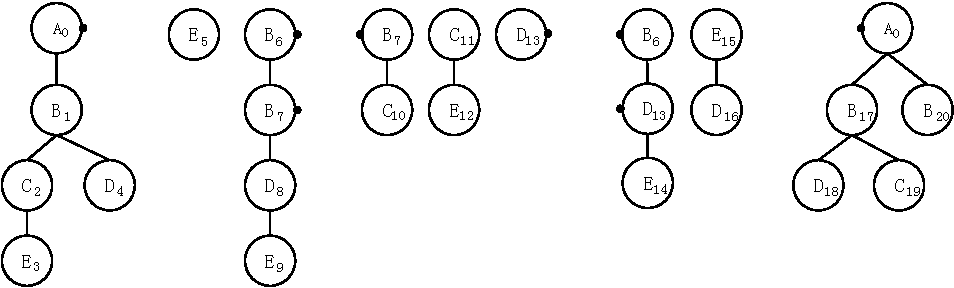
\includegraphics[]{partialtree/figures/fromWord-6.pdf}
	\caption{Subtrees from parsing chunks}
	\label{fig:partialtree-notfinished}
\end{figure*}


\subsection{Pre-path Computation}

The key idea of computing the pre-path for each partial tree is to make use
of open nodes. This is because the missing parent and ancestor nodes are caused
by splitting those nodes. Therefore, the information needed for creating the
pre-paths lies in them.

Algorithm 0 outlines the pseudo codes for computing pre-path. Since one chunk
may generate more than one subtrees, the input is a list of subtree lists. The
length of the list is equal to the number of partial trees, i.e. one chunk makes
one list of subtree, thus representing the length as $P$.

Algorithm 0 has three phases. In the first phase, it selects all the left-open
nodes into $LLS$ and all the right-open nodes into $RLS$ (line 2-4). $LLS_{[P]}$
collects the left-open nodes of the $p$th partial tree, likewise we have
$RLS_{[P]}$. Note that the nodes in $LLS_{[P]}$ or $RLS_{[P]}$ are arranged in
order from the root to leaves. For example, in Table~\ref{table:opennodes}, we
select all the open nodes and add them to corresponding lists.

{
	\setstretch{1.5}
\begin{figure}[!t]
 	\centering
 	\label{fig:ppalgorithm}
 	\begin{tabular}{l}
 		\hline
 		\hline
 		\makebox[.95\linewidth][l]{\textbf{Algorithm 0} \textsc{GetPrepath}($\mathit{STS}$)} \\
 		\hline
 		\textbf{Input}: $\mathit{STS}$: a list of subtree lists \\
 		\textbf{Output}: an list of partial trees\\
 		\makebox[1em][r]{1:}\hspace{1 mm} /* open nodes in LLS or RLS are arranged in top-bottom order */\\
 		\makebox[1em][r]{2:}\hspace{1 mm} \textbf{for all} $p \in [0, P)$ \textbf{do} \\
 		\makebox[1em][r]{3:}\hspace{4 mm} $\INDEXSETL{LLS} \leftarrow \mathit{SelectLeftOpenNodes}(\INDEXSETL{STS})$\\
 		\makebox[1em][r]{4:}\hspace{4 mm} $\INDEXSETL{RLS} \leftarrow \mathit{SelectRightOpenNodes}(\INDEXSETL{STS})$\\

 		\makebox[1em][r]{5:}\hspace{1 mm} /* Prepath-computation and collecting matching nodes */\\
 		\makebox[1em][r]{6:}\hspace{1 mm} $AuxList \leftarrow []$ \\
 		\makebox[1em][r]{7:}\hspace{1 mm} \textbf{for} $ p \in [0, P-1) $ \textbf{do}\\
 		\makebox[1em][r]{8:}\hspace{4 mm} $AuxList.\mathit{AppendToHead}(\INDEXSETL{RLS})$\\
 		\makebox[1em][r]{9:}\hspace{4 mm} $AuxList.\mathit{RemoveLast}(LLS_{[p+1]}.\mathit{Size}()) $\\
 		\makebox[1em][r]{10:}\hspace{4 mm} $ PPS_{[p+1]}\leftarrow AuxList$ \\

 		\makebox[1em][r]{11:}\hspace{1 mm}  /* Add pre-nodes to subtrees */ \\
 		\makebox[1em][r]{12:}\hspace{1 mm} $PTS \leftarrow []$ \\
 		\makebox[1em][r]{13:}\hspace{1 mm} \textbf{for} $ p \in [0, P) $ \textbf{do}\\
 		\makebox[1em][r]{14:}\hspace{4 mm} \textbf{for} $ i \in [0, PPS_{[p]}.Size() - 1)$ \textbf{do} \\
 		\makebox[1em][r]{15:}\hspace{8 mm}   $PPS_{[p][i]}.children.$Add$(PPS_{[p][i+1]})$ \\
  		\makebox[1em][r]{16:}\hspace{4 mm} $PPS_{[p]}.last.children.$Add$(\INDEXSETL{STS})$ \\
 		\makebox[1em][r]{17:}\hspace{4 mm}   $\INDEXSETL{PTS} \leftarrow PPS_{[p][0]}$ \\
 		\makebox[1em][r]{18:}\hspace{1 mm} \textbf{return} \emph{PTS} \\
 		\hline
 	\end{tabular}
 \end{figure}
}

In the second phase, we perform the pre-path computation. Once we split an XML
document from a position inside the document, the two partial trees created from
the splitting have the same number of open nodes on the splitting side. Given
two consecutive partial trees, the number of the right-open nodes of the left
partial tree is the same as the number of the left-open nodes of the right
partial tree. This is a very important feature and we exploit it for computing
the pre-paths of partial trees.

In the algorithm, we first add the $p$th $RLS$ to the head of an auxiliary list
$AuxList$ (line 8), and then we remove the same number of nodes as the number of
$(p-1)$th $LLS$ (line 9). Last, we keep the nodes in the $AuxList$ to the
$(p+1)$th $PPS$, which holds the pre-nodes for each partial tree.
Table~\ref{table:tempresult} shows the results of pre-path computation for the
given example.

{
\setstretch{1.5}
\begin{table}[t]
	\caption{Open node lists}
	\label{table:opennodes}
	\centering
	\begin{tabular}{c|cc}
		\hline
		& Left-open nodes	& Right-open nodes \\
		\hline
		pt$_0$	& []			& [A$_0$] \\
		pt$_1$	& []			& [B$_6$, B$_7$] \\
		pt$_2$	& [B$_7$]			& [D$_1$$_3$] \\
		pt$_3$	& [B$_6$, D$_1$$_3$]		& [] \\
		pt$_4$	& [A$_0$]			& [] \\
		\hline
	\end{tabular}

	\caption{Results of pre-path computation in AUX}
	\label{table:tempresult}
	\centering
	\begin{tabular}{c|ccc}
		\hline
		& Left-open nodes	& Right-open nodes & $AUX$\\
		\hline
		pt$_0$	& []			& [A$_0$]  & []\\
		pt$_1$	& []			& [B$_6$, B$_7$] & [A$_0$] \\
		pt$_2$	& [B$_7$]			& [D13] &[A$_0$,B$_6$]\\
		pt$_3$	& [B$_7$, D$_1$$_3$]		& []  & [A$_0$]\\
		pt$_4$	& [A$_0$]			& [] &[]\\
		\hline
	\end{tabular}
\end{table}
}

In last phase, we add the resultant pre-nodes to the corresponding partial trees
and copy the nodes from $PPS_{[p]}$ to $PTS_{[p]}$ as the results for output.
Because the pre-nodes in the pre-path are also open nodes, we list all open
nodes for each partial trees in Table~\ref{table:allopennodes}. Then, the
pre-path computation is complete. For the given example, we obtain the partial
trees as shown in Fig.~\ref{fig:partialtree2}.


\subsection{Creation of Ranges of Open Nodes}
\label{sec:ranges}

Once an XML node is split, it generates two or more open nodes of the same node
in consecutive partial trees. For example, as we can see in
Fig.~\ref{fig:partialtree2}, \Nr{B}{6} on pt$_1$, \Np{B}{6} on pt$_2$, and
\Nl{B}{6}  on pt$_3$ are created from the same node \Nc{B}{6}. For locating the
open nodes of the same node,  which are distrubted in different partial trees,
we use two integers \textit{start} and \textit{end} for an open node. With these
two integers, we can know the partial trees that have matching nodes of the same
open node. Note that after adding nodes to a partial tree, the open nodes from
the same node also have the same depth. Therefore, we can locate all the
matching nodes to set \textit{start} and \textit{end} for each open node. After
computation, we obtain the ranges of nodes as shown in
Table~\ref{table:rangesresult}.

{
	\setstretch{1.5}
\begin{table}[t]
		\caption{All open nodes}
	\label{table:allopennodes}
	\centering
	\begin{tabular}{c|cc}
		\hline
		& Left-open nodes	& Right-open nodes \\
		\hline
		pt$_0$	& []						& [A$_0$] \\
		pt$_1$	& [A$_0$]					& [A$_0$, B$_6$, B$_7$] \\
		pt$_2$	& [A$_0$, B$_6$, B$_7$]		& [A$_0$, B$_6$, D$_1$$_3$] \\
		pt$_3$	& [A$_0$, B$_6$, D$_1$$_3$]	& [A$_0$] \\
		pt$_4$	& [A$_0$]					& [] \\
		\hline
	\end{tabular}

	\caption{Open node lists with ranges}
	\label{table:rangesresult}
	\centering
	\begin{tabular}{c|cc}
		\hline
		& Left open nodes	& Right open nodes \\
		\hline
		pt$_0$	& []	& [A$_0$(0,4)] \\
		pt$_1$	& [A$_0$(0,4)]	& [A$_0$(0,4), B$_6$(1,3), B$_7$(1,2)] \\
		pt$_2$	& [A$_0$(0,4), B$_6$(1,3), B$_7$(1,2)]	& [A$_0$(0,4), B$_6$(1,3), D$_1$$_3$(2,3)] \\
		pt$_3$	& [A$_0$(0,4), B$_6$(1,3), D$_1$$_3$(2,3)]	& [A$_0$(0,4)] \\
		pt$_4$	& [A$_0$(0,4)]	& [] \\
		\hline
	\end{tabular}
\end{table}
}

By using these ranges, we can esaily establish the partial trees for the
matching nodes of the same node. For example, the range of A$_0$ is (0, 4), that
means we can locate the same nodes of \Nc{A}{0} from pt$_0$ to pt$_4$. As we can
see, there are \Nr{A}{0}, \Np{A}{0}, \Np{A}{0}, \Np{A}{0}, and \Nr{A}{0} on
pt$_0$ to pt$_4$, respectively.

%
%\section{Eavalute XPath Queries on Partial Trees}
\label{sec:queryalgo}

When performing an XPath query on an XML document, the evaluation is done on a
single tree. By exploiting partial tree, the evaluation of an XPath query on a
single tree is then applied to multiple partial trees. A significant advantagte
of using partial tree is that it makes the parallelization of evaluation of
XPath queries possible by simply evaluting the same query on partail trees
separately. However, it also brings challenges in designing query algorhtms on
partial trees. Generally speaking, there are three main difficulties as follows.

First, since partial trees are craeted from chunks of an XML document, a node
may be seperated and thus lie in different partial trees. This leads to a
possible situation that multiple open nodes may stem from the same node and
distributed in different partial trees as discussed in Section~\ref{sec:ranges}.
Since these open nodes are from the same node, in case when one of such open
nodes is selected in a partial tree (e.g., \Nr{B}{6} on \PT1), the other
corresponding nodes (\Np{B}{6} on \PT2 and \Nl{B}{6} on \PT3) should also be
selected for consistency. This is simply because they are all \Nc{B}{6} in the
original XML document.

Second, although partial trees have all the parent-child edges of their nodes,
the sibling-relation that is split among partial trees may be missing. For
example,  \Nc{B}{1} has five following-sibling nodes in the original XML tree,
but in \PT1, there is no following-sibling nodes of \Nc{B}{1} because of
splitting. When we perform queries with \texttt{following-sibling} or
\texttt{preceding-sibling}, the results may be in another (possibly far) partial
tree. We  design an algorithm to let the partial trees know about such cases.

Third, when we perform queries with a predicate, we usually execute the
sub-query in the predicate from a set of matching nodes.  However, on a set of
partial trees, the starting nodes and the matching nodes of the sub-query may be
on different partial trees (we will show this in the follwoing part of this
section). We also need an algorithm to propagate the information over partial
trees for queries with predicates.

In this section, we develop algorithms for evaluating XPath queries on a set of
partial trees. We first show the outline of the algorithms and then describe the
details of how the query algorithms work for evaluating XPath queries. We use
the following three XPath expressions as our running examples.

Q1: \texttt{ /child::A/descendant::B/descendant::C/parent::B}

Q2: \texttt{ /descendant::B/following-sibling::B}

Q3:  \texttt{ /descendant::B[following-sibling::B/child::C]/child::C}

After the introduction of the algorithms, we also discuss the complexity of our
algorithms at the end of this section.


\subsection{Definitions}

For introducing the query algorithms, we first give a few definitions to partial
tree nodes. Each node has a \textit{type} denoting its node type, including
closed, left-open, right-open and pre-node, and \textit{depth} denoting the
number of edges from the node to the root. A node has four pointers pointing to
the related nodes: the \textit{parent} pointer that points to its parent and the
\textit{children} pointer to its children. For accessing siblings, it has the
\textit{presib} pointer and the \textit{folsib} pointer that points to its
preceding-sibling node and following-sibling node, respectively. For
distinguishing nodes, we give each node a unique id called \textit{uid}.

Besides the partial tree node, there is also a requirement that we need to know
from which partial tree a node comes in distributed memory environments;
therefore, we number each partial tree with a unique id denoted as
\textit{partial tree id} or simply \textit{ptid} for distinguishing partial
trees. We number \textit{ptid} from 0 to \textit{P - 1} (where P is the total
number of partial trees) in document order.

For locating any node on a partial tree, we define data type \textit{Link} that
holds a ptid and a uid. By using \textsc{FindNode}(\textit{pt}, \textit{uid}),
we can locate any node with a unique integer \textit{uid} on partial tree
\textit{pt}. We assume that we can access any node in constant time.

When processing an XPath query, we evaluate it step by step in order. For
storing the results of a step, we define a resultant list of nodes for each
partial tree i.e. the are P reslultant lists given P partial trees. The
evaluation of a step is applies to each node in the resultant list. To start
with, we add a virtual node VN$i$ into a resultant list for each parital tree,
which has the root of PT$i$ as its single child. For example, VN$_0$ has only a
single child \Nr{A}{0} of \PT0 and is put into the resultant list before the
evaluation on \PT0 starts. The evaluation of a step generats a new resultant
list of nodes. After the evaluation, we replace the current resultant list with
the new list as the results and will be used as the input for the next step.


\subsection{Queries without Predicate}

Algorithm~1 outlines the big picture of our XPath query algorithms. The input
includes an XPath query to be evaluated and a set of partial trees generated
from an XML document. The output is a set of resultant nodes that matchs the
XPath query, each of which is associated with a corresponding partial tree.

The evaluation of the XPath query starts from the root of the original XML tree.
In case of paritial tree, the root node of the original tree corresponds to the
root node of every partial tree, and they are put into the resultant lists for
holding intermediate results (lines 1--2). Hereafter, the loops by $p$ over $[0,
P)$ are assumed to be executed in parallel.

As we know, an XPath query consists of one or more location steps, and in our
algorithm they are processed one by one in order. For each step, Algorithm~1
calls the corresponding sub-algorithm based on the axis of the step and updates
the intermediate results (line 4) in the resultant lists for each turn. Lines
6--9 will be executed in case the input XPath query has a predicates. We will
explain this part later in Section~\ref{sec:predicate}.

{
	\setstretch{1.5}
\begin{figure}[t]
  \label{fig:algQuery2}
	\centering
	\begin{tabular}{l}
		\hline
		\hline
		\makebox[.95\linewidth][l]{\textbf{Algorithm 1} \textsc{Query}($\mathit{steps}$, $\INDEXSET{pt}$)} \\
		\hline
		\textbf{Input}:           $\mathit{steps}$: an XPath expression \\
                \phantom{\textbf{Input}:} $\INDEXSET{pt}$: an indexed set of partial trees \\
		\textbf{Output}: an indexed set of results of query \\
		\makebox[1em][r]{1:}\hspace{1 mm} \textbf{for} $p \in [0, P)$ \textbf{do} \\
		\makebox[1em][r]{2:}\hspace{4 mm}    $\mathit{ResultList}_p \leftarrow \{~ \mathit{pt}_p.\mathit{root} ~\}$ \\
		\makebox[1em][r]{3:}\hspace{1 mm} \textbf{for all} $\emph{step} \in \emph{steps}$ \textbf{do} \\
		\makebox[1em][r]{4:}\hspace{4 mm}    $\INDEXSET{ResultList}$ \\
                \makebox[1em][r]{  }\hspace{6 mm}        ${}\leftarrow \hbox{\textsc{Query}}\langle\mathit{step}.\mathit{axis}\rangle(\INDEXSET{pt}, \INDEXSET{ResultList}, \mathit{step}.\mathit{test})$ \\
		\makebox[1em][r]{5:}\hspace{4 mm}    \textbf{if} $step.predicate \neq \hbox{\textsc{null}}$ \textbf{then} \\
		\makebox[1em][r]{6:}\hspace{7 mm}       $\INDEXSET{PResultList} \leftarrow \hbox{\textsc{PreparePredicate}}(\INDEXSET{ResultList})$ \\
		\makebox[1em][r]{7:}\hspace{7 mm}       \textbf{for all} $\emph{pstep} \in \emph{step.predicate}$ \textbf{do} \\
		\makebox[1em][r]{8:}\hspace{10 mm}         $\INDEXSET{PResultList}$ \\
                \makebox[1em][r]{  }\hspace{12 mm}             ${} \leftarrow  \hbox{\textsc{PQuery}}\langle\mathit{step}.\mathit{axis}\rangle(\INDEXSET{pt}, \INDEXSET{PResultList}, \mathit{pstep})$ \\
		\makebox[1em][r]{9:}\hspace{7 mm}       $\INDEXSET{ResultList} \leftarrow \hbox{\textsc{ProcessPredicate}}(\INDEXSET{PResultList})$ \\
		\makebox[1em][r]{10:}\hspace{1 mm} \textbf{return} $\INDEXSET{ResultList}$ \\
		\hline
	\end{tabular}
  \caption{Overall algorithm of XPath query for partial trees}
\end{figure}
}


\subsubsection{Downwards Axes}

Algorithm 2 shows the procedure for evaluting a step with a child axis. The
input $\INDEXSET{InputList}$ has the nodes selected up from the last step on
each partial tree. The algorithm simply lists up all the children of input nodes
and compares their tags with the node test (lines 3--4).

Algorithm 3 shows the procedure for evaluting a step with a descendant axis.
Starting from every node in the input, it traverses partial trees by depth-first
search along with a stack. To avoid redundant traversals on the same node, we
add the $\mathit{isChecked}$ flag for each node (lines 8--9) so that we can
evaluate  each node only once. Note that we can reduce the worst-case complexity
by using this flag from square to linear with respect to the number of nodes.

{
	\setstretch{1.5}
\begin{figure}[!t]
	\centering
	\begin{tabular}{l}
		\hline
		\hline
		\makebox[.95\linewidth][l]{\textbf{Algorithm 2} \textsc{Query}$\langle$\texttt{child}$\rangle$($\INDEXSET{pt}$, $\INDEXSET{InputList}$, $\mathit{test}$)} \\
		\hline
		\textbf{Input}:           $\INDEXSET{pt}$: an indexed set of partial trees \\
                \phantom{\textbf{Input}:} $\INDEXSET{InputList}$: an indexed set of input nodes \\
                \phantom{\textbf{Input}:} $\mathit{test}$: a string of nametest \\
		\textbf{Output}: an indexed set of results \\
		\makebox[1em][r]{1:}\hspace{1 mm} \textbf{for} $p \in [0, P)$ \textbf{do} \\
		\makebox[1em][r]{2:}\hspace{4 mm}    $\mathit{OutputList}_p \leftarrow [] $ \\
		\makebox[1em][r]{3:}\hspace{4 mm}    \textbf{for all} $n \in InputList_p$ \textbf{do} \\
		\makebox[1em][r]{4:}\hspace{7 mm}       $\mathit{OutputList}_p $ \\
                \makebox[1em][r]{  }\hspace{9 mm}          ${}\leftarrow \mathit{OutputList}_p \cup [nc ~|~ nc \in n.\mathit{children}, nc.\mathit{tag} = \mathit{test}] $ \\
		\makebox[1em][r]{5:}\hspace{1 mm} \textbf{return} $\INDEXSET{OutputList}$ \\
		\hline
        \\
		\hline
		\hline
		\makebox[.95\linewidth][l]{\textbf{Algorithm 3} \textsc{Query}$\langle$\texttt{descendant}$\rangle$($\INDEXSET{pt}$, $\INDEXSET{InputList}$, $\mathit{test}$)} \\
		\hline
		\textbf{Input}:           $\INDEXSET{pt}$: an indexed set of partial trees \\
                \phantom{\textbf{Input}:} $\INDEXSET{InputList}$: an indexed set of input nodes \\
                \phantom{\textbf{Input}:} $\mathit{test}$: a string of nametest \\
		\textbf{Output}: an indexed set of results \\
		\makebox[1em][r]{1:}\hspace{1 mm} \textbf{for} $p \in [0, P)$ \textbf{do} \\
		\makebox[1em][r]{2:}\hspace{4 mm}    $\mathrm{SetIsChecked}(\mathit{pt}_p, \mathit{false})$ \\
		\makebox[1em][r]{3:}\hspace{4 mm}    $\mathit{OutputList} \leftarrow [] $ \\
		\makebox[1em][r]{4:}\hspace{4 mm}    \textbf{for all} $n \in InputList_p$ \textbf{do} \\
		\makebox[1em][r]{5:}\hspace{7 mm}       $\mathit{Stack} \leftarrow \{ \emph{n} \}$ \\
		\makebox[1em][r]{6:}\hspace{7 mm}       \textbf{while not }$\mathit{Stack}.\mathit{Empty()}$ \textbf{do}  \\
		\makebox[1em][r]{7:}\hspace{10mm}         $nt \leftarrow \mathit{Stack}.\mathit{Pop}()$  \\
		\makebox[1em][r]{8:}\hspace{10mm}         \textbf{if} $nt.\mathit{isChecked}$ \textbf{then} \textbf{continue} \\
		\makebox[1em][r]{9:}\hspace{10mm}         $nt.\mathit{isChecked} \leftarrow \hbox{\textsc{true}}$ \\
		\makebox[1em][r]{10:}\hspace{10mm}         $\mathit{OutputList}_p $ \\
                \makebox[1em][r]{   }\hspace{12mm}             ${}\leftarrow \mathit{OutputList}_p \cup [nc ~|~ nc \in nt.children, nc.\mathit{tag} = \mathit{test}] $ \\
		\makebox[1em][r]{11:}\hspace{10mm}         $\mathit{Stack}.\mathit{PushAll}(nt.\mathit{children})$ \\
		\makebox[1em][r]{12:}\hspace{1 mm} \textbf{return} $\INDEXSET{OutputList}$ \\
		\hline
	\end{tabular}
    \caption{Query algorithm for downwards axes}
	\label{fig:algQueryChild2}
\end{figure}
}

Now let us look at our running example Q1. The process of downward steps of Q1
is listed in Table~\ref{tab:Q1first}. For the first step \texttt{child::A},
since  VN$_i$ has only one child that is the root of the $i$th partial tree, we
obtain it as the results for each partial tree as shown in the second row of the
table. Then we perform the next step \texttt{descendant::B} independently for
each partial tree from the results of the first step. We evalute the step
\texttt{descendant::B} on each of the nodes in the resultant list of the
previous step. For example, for \Nr{A}{1} on \PT1, there is only a node
\Nc{B}{1} that matches the query and is then selected and put into a new list.
As introduced, when the evaluation is done, the new list replaces the current
resultant list to be the resultant list up to the current step. The results of
this step for each partial tree are listed in the fourth row of
Table~\ref{tab:Q1first}.  For the third step \texttt{descendant::C}, the
algorithm works in a similar way. The results up to \texttt{descendant::C} are
lised in the last row of Table~\ref{tab:Q1first}. It is worth noting that the
$\mathit{isChecked}$ flag now works. For example, on \PT1, starting from
\Nr{B}{6}, we traverse \Nr{B}{7}, \Nc{D}{8}, \Nc{E}{9}, and then starting from
\Nr{B}{7}, we can stop the traversal immediately.

{
\setstretch{1.5}
\begin{table}[t]
\caption{Evaluating downward steps of Q1}
\label{tab:Q1first}
\begin{center}
\begin{tabular}{c|ccccc}
\hline
\hline
Process &
\PT0 &
\PT1 &
\PT2 &
\PT3 &
\PT4 \\
\hline
Input&
[VN$_0$] &
[VN$_1$] &
[VN$_2$] &
[VN$_3$] &
[VN$_4$] \\
\hline
\texttt{child::A} &
$ [\Nr{A}{0}] $ &
$ [\Np{A}{0}] $ &
$ [\Np{A}{0}] $ &
$ [\Np{A}{0}] $ &
$ [\Nl{A}{0}] $ \\
\hline
\texttt{descendant::B} &
$ [\Nc{B}{1}] $ &
$ [\Nr{B}{6}, \Nr{B}{7}] $ &
$ [\Np{B}{6}, \Nl{B}{7}] $ &
$ [\Nl{B}{6}] $ &
$ [\Nc{B}{17}, \Nc{B}{20}] $ \\
\hline
\texttt{descendant::C} &
$ [\Nc{C}{2}] $ &
$ [\,] $ &
$ [\Nc{C}{10}, \Nc{C}{11}] $ &
$ [\,] $ &
$ [\Nc{C}{19}] $ \\
\hline
\end{tabular}
\label{tab:Q1}
\end{center}
\end{table}
}

\subsubsection{Upwards Axes}

In querying of a step with downward axes, the algorithms have nothing different
to partial trees compared to ordinary XML trees. This is due to Property 1 in
Section~\ref{sec:chars}. Let an open node $x$ be selected after a downwards
query. Then, it should have started from an open node (this is an ancestor of
$x$) and the corresponding nodes should have all been selected, which means all
the nodes corresponding to $x$ should be selected after the query.

However, this discussion does not hold for the queries with upwards axes. In
such case when an open node is selected after an upwards query, it may come
from a closed node and we have no guarantee that all the corresponding open
nodes are selected. Therefore, we add a postprocessing for sharing the selected
nodes when we process the upwards axes.

Algorithm 4 shows the procedure for evaluating a step with a parent axis.
It has almost the same flow as that of the child axis (lines 1--5),
except for the last call of the \textsc{ShareNodes} function.

The \textsc{ShareNodes} function is used for keeping the consistency of open
nodes. It consists of two parts\footnote{In our implementation of this
\textsc{ShareNodes} function, there are two phases of communication: all the
partial trees send their open nodes to a process and then the necessary data for
a partial tree are sent back.}.

First, it collects all the selected open nodes from all partial trees (lines
4--6). Then, based on the range information of node $n$ ($n.\mathit{start}$ and
$n.\mathit{end}$), we add all the corresponding selected nodes to all the
partial trees. After the call of \textsc{ShareNodes} function, all the open
nodes that are from the same node are selected in corresponding partial trees.

Now, let us continue the running example Q1 for its last step as shown in
Table~\ref{tab:Q1last}. For the \texttt{parent::B} after the
\texttt{descendant::C}, we first directly select the parent nodes of the
intermediate results from the results of the previous step independently. For
the running example, we can notice that \Nc{B}{1} is selected for it is  the
parent of \Nc{C}{2} on \PT0, while for \Nl{B}{7} and \Np{B}{6}, they are the
parents of \Nc{C}{10} and \Nc{C}{11} respectively.  The results are listed in
the second row of Table\ref{tab:Q1last}.

Here, unfortunately the node \Nl{B}{7} is selected on \PT2, but its
corresponding node on \PT1, i.e. \Nr{B}{7}, has not been selected yet.  We then
call the \textsc{ShareNodes} function. By collecting all the open nodes from all
the partial trees, we have the list $[\Nl{B}{7}, \Np{B}{6}]$. Since they have
ranges $(1, 2)$ and $(1, 3)$, respectively, \PT1 receives two nodes \Nr{B}{7}
and \Nr{B}{6}, \PT2 receives two nodes \Nl{B}{7} and \Np{B}{6}, and \PT3
receives one node \Nl{B}{6}. By taking the union with the previous intermediate
results, we obtain the final results as shown in the last row of
Table\ref{tab:Q1last}.

Now, after evaluating the last step of Q1, the evaluation of the whole query Q1
is complete. The resultant lists in the last row of the table from evaluating
the last step is then the final results of Q1.

{
	\setstretch{1.5}
\begin{table}[t]
	\caption{Evaluating the last step of Q1}
	\label{tab:Q1last}
	\begin{center}
		\medskip
		\begin{tabular}{c|ccccc}
			\hline
			\hline
			Process &
			\PT0 &
			\PT1 &
			\PT2 &
			\PT3 &
			\PT4 \\
			\hline
			Input &
			$ [\Nc{C}{2}] $ &
			$ [\,] $ &
			$ [\Nc{C}{10}, \Nc{C}{11}] $ &
			$ [\,] $ &
			$ [\Nc{C}{19}] $ \\
			\hline
			\texttt{parent::B} &
			$ [\Nc{B}{1}] $ &
			$ [\,] $ &
			$ [\Nl{B}{7}, \Np{B}{6}] $ &
			$ [\,] $ &
			$ [\Nc{B}{17}] $ \\
			\hline
			\textsc{ShareNode} &
			$ [\Nc{B}{1}] $ &
			$ [\Nr{B}{6}, \Nr{B}{7}] $ &
			$ [\Nl{B}{7}, \Np{B}{6}] $ &
			$ [\Nl{B}{6}] $ &
			$ [\Nc{B}{17}] $ \\
			\hline
		\end{tabular}
		\medskip
	\end{center}
\end{table}

\begin{figure}[t]
	\centering
	\begin{tabular}{l}
		\hline
		\hline
		\makebox[.95\linewidth][l]{\textbf{Algorithm 4} \textsc{Query}$\langle$\texttt{parent}$\rangle$($\INDEXSET{pt}$, $\INDEXSET{InputList}$, $\mathit{test}$)} \\
		\hline
		\textbf{Input}:           $\INDEXSET{pt}$: an indexed set of partial trees \\
        \phantom{\textbf{Input}:} $\INDEXSET{InputList}$: an indexed set of input nodes \\
        \phantom{\textbf{Input}:} $\mathit{test}$: a string of nametest \\
		\textbf{Output}: an indexed set of results \\
		\makebox[1em][r]{1:}\hspace{1 mm} \textbf{for} $p \in [0, P)$ \textbf{do} \\
		\makebox[1em][r]{2:}\hspace{4 mm}    $\mathit{OutputList}_p \leftarrow [\,]$ \\
		\makebox[1em][r]{3:}\hspace{4 mm}    \textbf{for all} $n \in \mathit{InputList}_p$ \textbf{do} \\
		\makebox[1em][r]{4:}\hspace{7 mm}       \textbf{if} $n.\mathit{parent} \neq \hbox{\textsc{null}}$ \textbf{ and } $n.\mathit{parent}.\mathit{tag} = \emph{test}$ \textbf{then} \\
		\makebox[1em][r]{5:}\hspace{10mm}          $\mathit{OutputList}_p.\mathit{Add}(n)$ \\
		\makebox[1em][r]{6:}\hspace{1 mm} \textbf{return} \textsc{ShareNodes}($\INDEXSET{pt}$, $\INDEXSET{OutputList}$) \\
		\hline
        \\
        \hline
		\hline
		\makebox[.95\linewidth][l]{\textbf{Algorithms 5} \textsc{ShareNodes}($\INDEXSET{pt}$, $\INDEXSET{NodeList})$} \\
		\hline
		\textbf{Input}:           $\INDEXSET{pt}$: an indexed set of partial trees \\
                \phantom{\textbf{Input}:} $\INDEXSET{NodeList}$: an indexed set of nodes \\
		\textbf{Output}: an indexed set of nodes after sharing\\
		\makebox[1em][r]{1:}\hspace{1 mm} /* Select all open nodes and append them to a node list */ \\
		\makebox[1em][r]{2:}\hspace{1 mm} $\mathit{ToBeShared} \leftarrow [\,]$ \\
		\makebox[1em][r]{3:}\hspace{1 mm} \textbf{for} $p \in [0, P)$ \textbf{do} \\
		\makebox[1em][r]{4:}\hspace{4 mm} $ \mathit{OpenNodes} \leftarrow [n ~|~ n \in \mathit{NodeList}_p, $\\
		\makebox[1em][r]{5:}\hspace{4 mm} \phantom{$ \mathit{OpenNodes} \leftarrow [n ~|~$}$n.\mathit{type} \in \{\textsc{LeftOpen}, \textsc{RightOpen}, \textsc{PreNode}\}]$\\
		\makebox[1em][r]{6:}\hspace{4 mm} $ \mathit{ToBeShared} \leftarrow \mathit{ToBeShared} \cup \mathit{OpenNodes}$ \\[5pt]
		\makebox[1em][r]{7:}\hspace{1 mm} /* Regroup nodes by partial tree id and add them to NodeList */ \\
		\makebox[1em][r]{8:}\hspace{1 mm} \textbf{for} $p \in [0, P)$ \textbf{do} \\
		\makebox[1em][r]{9:}\hspace{4 mm}    $\mathit{ToBeAdded}_p \leftarrow [n ~|~ n \in \mathit{ToBeShared}, n.\mathit{start} \le p \le n.\mathit{end}]$ \\
		\makebox[1em][r]{10:}\hspace{4 mm}    $\mathit{OutputList}_p \leftarrow \mathit{NodeList}_p \cup \mathit{ToBeAdded}_p$ \\
		\makebox[1em][r]{11:}\hspace{1 mm} \textbf{return} $\INDEXSET{OutputList}$ \\
		\hline
	\end{tabular}
        \caption{Query algorithms for upwards axes}
	\label{fig:algQueryParent2}
\end{figure}
}

\subsubsection{Intra-sibling Axes}

The \texttt{following-sibling} or \texttt{preceding-sibling} axes retrieve nodes
from a set of nodes that are siblings of an intermediate node.  In our partial
trees, a set of those sibling nodes might be divided into two or more partial
trees. Therefore, these intro-sibling axes require querying on other partial
trees in addition to the local querying.

Without loss of generality, we discuss the following-sibling axis only, since
preceding-sibling is only different in a opposite direction compared to
following-sibling axis. Algorithm 6 shows the procedure for evaluating a step
with a following-sibling axis, which consists of four phases: local query,
preparation, regrouping, and remote query.

In the local query, we utilize the $\mathit{folsib}$ pointer and the
$\mathit{isChecked}$ flag to realize linear-time querying (lines 6--10). Then,
in the preparation, we select the nodes that are passed to another partial tree
to perform the remote query.  The latter two conditions (lines 14, 15) are
rather easy: we will ask a remote query if the parent node can have more
segments on the right (i.e., right open). The former condition (line 13) is a
little tricky.  Even if the latter two conditions hold, we do not need a remote
query if the node itself is right open.  Notice that if a node is right open
then it should have a corresponding left-open node in another partial tree, and
that node will ask for a remote query.  The regrouping is almost the same as
that in \textsc{ShareNodes}, and the difference is the range we consider (we
only look at the right for the following-sibling). Finally, the remote query
finds the children from the intermediate nodes given by regrouping.

Now, let us look at our running example of Q2. After the evaluation of
\texttt{descendant::B}, we have the intermediate results in the third row of
Table~\ref{tab:query2}. In the first phase of \texttt{following-sibling::B}, we get
the results in the third row. Then, we collect the parent nodes that satisfies
the conditions (lines 13--15). Such nodes and their ranges are: \Nr{A}{0} with
range [1,4] (on \PT0), \Np{B}{6} with range [3,3] (on \PT2), and \Np{A}{0} with
range [4,4] (on \PT3). By regrouping the nodes based on the partial tree id, the
input nodes for the remote query are as in the fourth row of the table. Starting
from these intermediate results, we select their children and obtain the results
as shown in the last row of Table~\ref{tab:query2}. Note that these results are also
the final results for the query since the result of a local query is a subset of
this remote query.

{
	\setstretch{1.5}
\begin{table}[t]
	\caption{Evaluating the location steps of Q2}
	\label{tab:query2}
\centering
\small
\begin{tabular}{c|ccccc}
\hline
\hline
Process &
\PT0 &
\PT1 &
\PT2 &
\PT3 &
\PT4 \\
\hline
Input&
[VN$_0$] &
[VN$_1$] &
[VN$_2$] &
[VN$_3$] &
[VN$_4$] \\
\hline
\texttt{descendant::B} &
$ [\Nc{B}{1}] $ &
$ [\Nr{B}{6}, \Nr{B}{7}] $ &
$ [\Np{B}{6}, \Nl{B}{7}] $ &
$ [\Nl{B}{6}] $ &
$ [\Nc{B}{17}, \Nc{B}{20}] $ \\
\hline
\texttt{following-sibling::B} &
$ [\,] $ &
$ [\,] $ &
$ [\,] $ &
$ [\,] $ &
$ [\Nc{B}{20}] $ \\
\hline
remote \texttt{Parent::A} &
$ [\,] $ &
$ [\Np{A}{0}] $ &
$ [\Np{A}{0}] $ &
$ [\Np{A}{0}, \Nl{B}{6}] $ &
$ [\Nl{A}{0}] $ \\
\hline
remote \texttt{child::B} &
$ [\,] $ &
$ [\Nr{B}{6}] $ &
$ [\Np{B}{6}] $ &
$ [\Nl{B}{6}] $ &
$ [\Nc{B}{17},\Nc{B}{20}] $ \\
\hline
\end{tabular}
\end{table}

\begin{figure}[!t]
	\centering
	\begin{tabular}{l}
		\hline
		\hline
		\makebox[.95\linewidth][l]{\textbf{Algorithm 6} \textsc{Query}$\langle$\texttt{following-sibling}$\rangle$($\INDEXSET{pt}$, $\INDEXSET{InputList}$, $\mathit{test}$)} \\
		\hline
		\textbf{Input}:           $\INDEXSET{pt}$: an indexed set of partial trees \\
                \phantom{\textbf{Input}:} $\INDEXSET{InputList}$: an indexed set of input nodes \\
                \phantom{\textbf{Input}:} $\mathit{test}$: a string of nametest \\
		\textbf{Output}: an indexed set of results \\
		\makebox[1em][r]{ 1:}\hspace{1 mm} \textbf{for} $p \in [0, P)$ \textbf{do} \\[5pt]
		\makebox[1em][r]{ 2:}\hspace{4 mm}    /* Local query */ \\
		\makebox[1em][r]{ 3:}\hspace{4 mm}    $\mathrm{SetIsChecked}(\mathit{pt}_p, \mathit{false})$ \\
		\makebox[1em][r]{ 4:}\hspace{4 mm}    $ \mathit{OutputList}_p \leftarrow [\,] $ \\
		\makebox[1em][r]{ 5:}\hspace{4 mm}    \textbf{for all} $n \in InputList_p$ \textbf{do} \\
		\makebox[1em][r]{ 6:}\hspace{7 mm}       \textbf{while} $n.\mathit{isChecked} = \hbox{\textsc{false}}$ \textbf{and} $n.folsib \neq \hbox{\textsc{null}}$ \textbf{do} \\
		\makebox[1em][r]{ 7:}\hspace{10mm}          $n.\mathit{isChecked} \leftarrow \hbox{\textsc{true}}$ \\
		\makebox[1em][r]{ 8:}\hspace{10mm}          $n \leftarrow n.folsib$ \\
		\makebox[1em][r]{ 9:}\hspace{10mm}          \textbf{if} $n.tag = test$ \textbf{then} \\
		\makebox[1em][r]{10:}\hspace{13mm}             $OutputList_p.\mathit{Add}(n)$ \\[5pt]
		\makebox[1em][r]{11:}\hspace{4 mm}    /* Preparing remote query */ \\
		\makebox[1em][r]{12:}\hspace{4 mm}    \textbf{for all} $n \in \mathit{InputList}_p$ \textbf{do} \\
		\makebox[1em][r]{13:}\hspace{7 mm}       \textbf{if} $n.type \not\in \{\hbox{\textsc{RightOpen}}, \hbox{\textsc{PreNode}}\}$ \\
		\makebox[1em][r]{14:}\hspace{9 mm}             \textbf{and} $n.\mathit{parent} \neq \hbox{\textsc{null}}$ \\
		\makebox[1em][r]{15:}\hspace{9 mm}             \textbf{and} $n.parent.type \in \{\hbox{\textsc{RightOpen}}, \hbox{\textsc{PreNode}}\}$ \textbf{then}\\
		\makebox[1em][r]{16:}\hspace{11 mm}                $\mathit{ToBeQueried}.\mathit{Add}((n.\mathit{parent}, p+1, n.\mathit{parent}.\mathit{end}))$ \\[5pt]
		\makebox[1em][r]{17:}\hspace{1 mm} /* Regroup nodes by partial tree id */\\
		\makebox[1em][r]{18:}\hspace{4 mm} \textbf{for} $p \in [0, P)$ \textbf{do}\\
		\makebox[1em][r]{19:}\hspace{7 mm}    $RemoteInput_p \leftarrow [n ~|~ (n, st, ed) \in \mathit{ToBeQueried}, st \le p \le ed] $ \\[5pt]
		\makebox[1em][r]{20:}\hspace{1 mm} /* Remote query */ \\
		\makebox[1em][r]{21:}\hspace{1 mm} $\INDEXSET{RemoteOutput} \leftarrow \hbox{\textsc{Query}$\langle$\texttt{child}$\rangle$($\INDEXSET{pt}$, $\INDEXSET{RemoteInput}$, $\mathit{test}$)}$ \\
		\makebox[1em][r]{22:}\hspace{1 mm} \textbf{for} $p \in [0, P)$ \textbf{do} \\
		\makebox[1em][r]{23:}\hspace{4 mm}    $ \mathit{OutputList}_p \leftarrow \mathit{OutputList}_p \cup \mathit{RemoteOutput}_p$ \\
		\makebox[1em][r]{24:}\hspace{0 mm} \textbf{return} $\INDEXSET{OutputList}$ \\
		\hline
	\end{tabular}
	\caption{Algorithm for Following-sibling axis}
	\label{fig:algQueryFolsib2}
\end{figure}
}


\subsection{Queries with Predicate}
\label{sec:predicate}

Predicates in this study are filters that check the existence of matched nodes
by simple steps that have no predicates. Our algorithm for handling predicates
consists of three phases: preparing, evaluating steps in predicates, and
processing predicates. The main differences of processing predicates are the
elements of their intermediate data. In the evaluation of steps, we select nodes
as we do for steps that have no predicates. In the querying in predicates, we
also attach a link to each of the original nodes from which the predicates are
evaluated. Since the upwards or intra-sibling axes may select a node on a
different partial tree, the link is a pair of partial tree id and the index of
nodes in the partial tree. The intermediate data will be denoted as $(x, (i,
y))$ in the pseudo code or as $\pred{x}{\PT{i}.y}$ in the running example, both
of which mean node $x$ is selected and it has a link to node $y$ on \PT{i}.

\subsubsection{Preparing Predicate}

Algorithm 7 shows the procedure for initializing the process of a predicate.
It just copies the nodes from the input lists with a link to the node itself.

For example in Q3, after evaluating \texttt{descendant::B}, we have the
resultant lists  before the predicate evaluation as shown in the third row of
Table~\ref{tab:q3prepare}. Then, by calling \textsc{PreparePredicate}, we have
the intermediate results as shown in the last row of the table. Note that (1)
all the links point to the nodes themselves at the beginning and (2) the
resultant lists in the last row of the table are newly created apart from the
current resultant list.

{
	\setstretch{1.5}
\begin{table}[t]
    \caption{Prepare the predicate of Q3}
    \label{tab:q3prepare}
\begin{center}\footnotesize
	\medskip
	\begin{tabular}{c|ccccc}
		\hline
		\hline
		Process &
		\PT0 &
		\PT1 &
		\PT2 &
		\PT3 &
		\PT4 \\
		\hline
		Input&
		[VN$_0$] &
		[VN$_1$] &
		[VN$_2$] &
		[VN$_3$] &
		[VN$_4$] \\
		\hline
		\texttt{descendant::B} &
		$ [\Nc{B}{1}] $ &
		$ [\Nr{B}{6},\Nr{B}{7}] $ &
		$ [\Np{B}{6},\Nl{B}{7}] $ &
		$ [\Nl{B}{6}] $ &
		$ [\Nc{B}{17},\Nc{B}{20}] $ \\
		\hline
		\hline
		Prepare &
		$ [\Nc{B}{1}\rightarrow $ &
		$ [\pred{\Nr{B}{6}}{\PT1.\Nr{B}{6}}, $ &
		$ [\pred{\Np{B}{6}}{\PT2.\Np{B}{6}}, $ &
		$ [\Nl{B}{6}\rightarrow $ &
		$ [\pred{\Nc{B}{17}}{\PT4.\Nc{B}{17}}, $ \\
		predicate &
		$ \{\PT0.\Nc{B}{1}\}] $ &
		$ \pred{\Nr{B}{7}}{\PT1.\Nr{B}{7}}] $ &
		$ \pred{\Nl{B}{7}}{\PT2.\Nl{B}{7}}] $ &
		$ \{\PT3.\Nl{B}{6}\}] $ &
		$ \pred{\Nc{B}{20}}{\PT4.\Nc{B}{20}}] $ \\
		\hline
	\end{tabular}
	\medskip
	\end{center}
\end{table}
}


\subsubsection{Evaluation of Steps within A Predicate}

The evaluation of inner steps of a prediate is almost the same as that without
predicate. Algorithm 9 shows the procedure for evalauting a step with a child
axis in the predicate; the key differences are the type of intermediate values
and the duplication of links.

There is another important difference for the descendant, ancestor,
following-sibling, and preceding-sibling. In the querying without predicate, we
used the $\mathit{isChecked}$ flag to avoid traversing the same node more than
once. In the querying in predicates, however, the different nodes may have
different links and this prevents us from using the flag. As we can see in the
discussion on complexity later, this modification makes the algorithm over
linear.

Now we continue our running example Q3 for the evaluation of the inner steps of
the prediate as shown in Table~\ref{tab:q3steps}. We then apply the query
\texttt{following-sibling::B} in two phases: the local query and the remote
query. The local query is the same as that of the previous section. The only
different is the nodes to be processed, which have links with them. We obtain
the results as shown in the third row of the table.

The remote queries are different from that is not in a predicate. Although
selected nodes are the same as before, they may have multiple links and are
stored in newly created lists. For example,  \Nc{B}{17} and \Nc{B}{20} in \PT4
both have two links. By merging results from local and remote queries, we
finally have the following intermediate results after
\texttt{following-sibling::B} in the predicate as shown in the fourth row of the
table.

For example, let us consider \Nc{B}{20} in \PT4. The local result of it is
$\pred{\Nc{B}{20}}{\PT4.\Nc{B}{20}}$, and the remote results is
$\pred{\Nc{B}{20}}{\PT0.\Nc{B}{1}, \PT3.\Nl{B}{6}}$. After merging link,  we
have $\pred{\Nc{B}{20}}{\PT0.\Nc{B}{1}, \PT3.\Nl{B}{6}, \PT4.\Nc{B}{20}}$ as
the result.

Similarly, by applying the following step \texttt{child::C}, the intermediate
results are shown in the last row of Table~\ref{tab:q3steps}. Note that in \PT4,
the resultant node $ [\pred{\Nc{C}{19}}{\PT0.\Nc{B}{1}, \PT3.\Nl{B}{6}}] $ is
a child of \Nc{B}{17}. Thus, it follows the link of \Nc{B}{17}.

{
	\setstretch{1.5}
\begin{table}[t]
	\caption{Evaluate inner steps of the predicate in Q3}
	\label{tab:q3steps}
	\centering
	\footnotesize
	\medskip
	\begin{tabular}{c|ccccc}
		\hline
		\hline
		Process &
		\PT0 &
		\PT1 &
		\PT2 &
		\PT3 &
		\PT4 \\
		\hline
		Input &
		$ [\Nc{B}{1}\rightarrow $ &
		$ [\pred{\Nr{B}{6}}{\PT1.\Nr{B}{6}}, $ &
		$ [\pred{\Np{B}{6}}{\PT2.\Np{B}{6}}, $ &
		$ [\Nl{B}{6}\rightarrow $ &
		$ [\pred{\Nc{B}{17}}{\PT4.\Nl{B}{17}}, $ \\
		&
		$ \{\PT0.\Nc{B}{1}\}] $ &
		$ \pred{\Nr{B}{7}}{\PT1.\Nr{B}{7}}] $ &
		$ \pred{\Nl{B}{7}}{\PT2.\Nl{B}{7}}] $ &
		$ \{\PT3.\Nl{B}{6}\}] $ &
		$ \pred{\Nc{B}{20}}{\PT4.\Nc{B}{20}}] $ \\
		\hline
		local &
		&
		&
		&
		&\\
		\texttt{following-}&
		$ [\,] $ &
		$ [\,] $ &
		$ [\,] $ &
		$ [\,] $ &	$ [\pred{\Nc{B}{20}}{\PT4.\Nl{B}{17}}] $ \\
		\texttt{sibling::B} &
		&
		&
		&
		&\\
		\hline
		\hline
		remote &
		$ [\,] $ & $ [\Nr{B}{6}\rightarrow $ &
		$ [\Np{B}{6}\rightarrow  $ &
		$ [\Nl{B}{6}\rightarrow $ &
		$ [\pred{\Nc{B}{17}}{\PT0.\Nc{B}{1}, \PT3.\Nl{B}{6}}$ \\
	    queries &
	    &
	    $\{\PT0.\Nc{B}{1}\}]$ &
	    $\{\PT0.\Nc{B}{1}\}]$  &
	    $\{\PT0.\Nc{B}{1}\}]$  &
	    $\pred{\Nc{B}{20}}{\PT0.\Nc{B}{1}, \PT3.\Nl{B}{6}}] $ \\
		\hline
		\hline
		merge link&
		$ [\,] $ & $ [\Nr{B}{6}\rightarrow $ &
		$ [\Np{B}{6}\rightarrow  $ &
		$ [\Nl{B}{6}\rightarrow $ &
		$ [\pred{\Nc{B}{17}}{\PT0.\Nc{B}{1}, \PT3.\Nl{B}{6}}, $ \\
		&
		&
		$\{\PT0.\Nc{B}{1}\}]$ &
		$\{\PT0.\Nc{B}{1}\}]$  &
		$\{\PT0.\Nc{B}{1}\}]$  &
		$ \Nc{B}{20} \rightarrow \{\PT0.\Nc{B}{1}, \PT3.\Nl{B}{6},$ \\
		&
		&
		&
		&
		& $ \PT4.\Nl{B}{17}\}] $\\
		\hline
		\texttt{child::C} &
		$ [\,] $ &
		$ [\,] $ &
		$ [\pred{\Nl{C}{11}}{\PT0.\Nc{B}{1}}] $ &
		$ [\,] $ &
		$ [\pred{\Nc{C}{19}}{\PT0.\Nc{B}{1}, \PT3.\Nl{B}{6}}] $ \\
		\hline
	\end{tabular}

	\medskip
\end{table}
}

\subsubsection{Processing Predicate}

Finally, we process the intermediate results to obtain the results after
filtering of predicate. Algorithm 8 shows the procedure for processing the
predicate.

The algorithm is similar to the \textsc{ShareNodes} function, but in this case
we consider all the results instead of open nodes. First, we collect all the
links (lines 3--4) and then select only the nodes that have at least one link to
the node (lines 5--6). Since there is no guarantee that all the corresponding
open nodes have been activated by predicates, we need an additional call of
\textsc{ShareNodes}.

For our running example Q3, the results are shown in the third row of
Table~\ref{tab:q3process}. Links $\pred{\Nc{C}{11}}{\PT0.\Nc{B}{1}}$ in the
intermediate results of \PT2 adds node \Nc{B}{1} to the result list of \PT0 and
$\pred{\Nc{C}{19}}{\PT0.\Nc{B}{1}, \PT3.\Nl{B}{6}}$ in the intermediate results
of \PT4 adds two nodes, \Nc{B}{1} on \PT0 and \Nl{B}{6} on \PT3, respectively.
We then apply the \textsc{ShareNodes} function and obtain the intermediate
results as in the second last row of Table~\ref{tab:q3process}.

The last step simply calls the processing of the step with a child axis, and the
final results for Q3 are in the last row of the table. Then, the query of Q3 is
complete. All the nodes in the resultant lists are the final results.


{
	\setstretch{1.5}
\begin{table}[t]
	\caption{Process the predicate in Q3}
	\label{tab:q3process}
	\centering
	\small
	\begin{tabular}{c|ccccc}
\hline
\hline
Process &
\PT0 &
\PT1 &
\PT2 &
\PT3 &
\PT4 \\
\hline
Input &
$ [\,] $ &
$ [\,] $ &
$ [\pred{\Nl{C}{11}}{\PT0.\Nc{B}{1}}] $ &
$ [\,] $ &
$ [\pred{\Nc{C}{19}}{\PT0.\Nc{B}{1}, \PT3.\Nl{B}{6}}] $ \\
\hline
\hline
Process predicate &
$ [\Nc{B}{1}] $ &
$ [\,] $ &
$ [\,] $ &
$ [\Nl{B}{6}] $ &
$ [\,] $ \\
\hline
\textsc{ShareNode} &
$ [\Nc{B}{1}] $ &
$ [\Nr{B}{6}] $ &
$ [\Np{B}{6}] $ &
$ [\Nl{B}{6}] $ &
$ [\,] $ \\
\hline
\texttt{child::C} &
$ [\Nc{C}{2}] $ &
$ [\,] $ &
$ [\Nc{C}{11}] $ &
$ [\,] $ &
$ [\,] $ \\
\hline
\end{tabular}
\medskip
\end{table}


\begin{figure}[t]
	\centering
	\begin{tabular}{l}
		\hline
		\hline
		\makebox[.95\linewidth][l]{\textbf{Algorithm 7} \textsc{PreparePredicate}($\INDEXSET{InputList}$)} \\
		\hline
		\textbf{Input}: $\INDEXSET{InputList}$: an indexed set of lists of nodes \\
		\textbf{Output}: an indexed set of lists of (node, link) \\
		\makebox[1em][r]{ 1:}\hspace{1 mm} \textbf{for} $i \in [0, P)$ \textbf{do} \\
		\makebox[1em][r]{ 2:}\hspace{4 mm} $\mathit{OutputList}_p \leftarrow [(n, (p, n.uid)) | n \in \mathit{InputList}_p]$ \\
		\makebox[1em][r]{ 3:}\hspace{1 mm} \textbf{return} \emph{OutputList} \\
		\hline
		\\
		\hline
		\hline
		\makebox[.95\linewidth][l]{\textbf{Algorithm 8} \textsc{ProcessPredicate}($\INDEXSET{pt}$, $\INDEXSET{InputList}$)} \\
		\hline
		\textbf{Input}:           $\INDEXSET{pt}$: an indexed set of partial trees \\
		\phantom{\textbf{Input}:} $\INDEXSET{InputList}$: an indexed set of lists of (node, link) \\
		\textbf{Output}: an indexed set of lists of filtered nodes \\
		\makebox[1em][r]{ 1:}\hspace{1 mm} /* regroup links by partial tree id. */ \\
		\makebox[1em][r]{ 2:}\hspace{1 mm} $\mathit{AllLinks} \leftarrow [\,]$ \\
		\makebox[1em][r]{ 3:}\hspace{1 mm} \textbf{for} $i \in [0, P)$ \textbf{do} \\
		\makebox[1em][r]{ 4:}\hspace{4 mm}    $\mathit{AllLinks} \leftarrow \mathit{AllLinks} \cup [(p', i') | (n', (p', i')) \in \mathit{InputList}_p]$ \\
		\makebox[1em][r]{ 5:}\hspace{1 mm} \textbf{for} $i \in [0, P)$ \textbf{do} \\
		\makebox[1em][r]{ 6:}\hspace{4 mm}    $\mathit{Activated}_p \leftarrow [n ~|~ (p', i') \in \mathit{AllLinks}, p = p', n.\mathit{uid} = i']$ \\[5pt]
		\makebox[1em][r]{ 7:}\hspace{1 mm} \textbf{return} \textsc{ShareNodes}($\INDEXSET{pt}$, $\INDEXSET{Activated}$) \\
		\hline
	\end{tabular}
	\caption{Query algorithm for handling predicate}
	\label{fig:funPredicate2}
\end{figure}

\begin{figure}[t]
	\centering
	\begin{tabular}{l}
		\hline
		\makebox[.95\linewidth][l]{\textbf{Algorithm 9} \textsc{PQuery}$\langle$\texttt{child}$\rangle$($\INDEXSET{pt}$, $\INDEXSET{InputList}$, $\INDEXSET{test}$)} \\
		\hline
		\textbf{Input}:           $\INDEXSET{pt}$: an indexed set of partial trees \\
		\phantom{\textbf{Input}:} $\INDEXSET{InputList}$: an indexed set of lists of (node, link) \\
		\phantom{\textbf{Input}:} $\mathit{test}$: a string of nametest \\
		\textbf{Output}: an indexed set of lists of (node, link) \\
		\makebox[1em][r]{1:}\hspace{1 mm} \textbf{for} $p \in [0, P)$ \textbf{do} \\
		\makebox[1em][r]{2:}\hspace{4 mm}    $\mathit{OutputList}_p \leftarrow [] $ \\
		\makebox[1em][r]{3:}\hspace{4 mm}    \textbf{for all} $(n, link) \in InputList_p$ \textbf{do} \\
		\makebox[1em][r]{4:}\hspace{7 mm}       $\mathit{OutputList}_p $ \\
		\makebox[1em][r]{  }\hspace{9 mm}          ${}\leftarrow \mathit{OutputList}_p \cup [(nc, link) ~|~ nc \in n.\mathit{children}, nc.\mathit{tag} = \mathit{test}] $ \\
		\makebox[1em][r]{5:}\hspace{1 mm} \textbf{return} $\INDEXSET{OutputList}$ \\
		\hline
	\end{tabular}
	\caption{Query algorithm for child axis in a predicate}
	\label{fig:algQueryPreChild2}
\end{figure}
}

\subsection{Worst-Case Complexity}

At the end of this section, we discuss the time complexity of our algorithms.
Here we analyze the worst-case complexity in the following categorization:

$\bullet$ axes,

$\bullet$ without or in predicate, and

$\bullet$ local computation and network communication.


For discussion, let $N$ be the total number of nodes in a given XML
document, $H$ be the tree height, and $P$ be the number of partial trees.
Assuming that the given document is evenly split,
the number of nodes in a chunk is $N/P$.
Each partial tree may have pre-path, which has at most $H$ extra nodes.
Therefore, the number of nodes in a partial tree is at most $N/P + H$.
The number of open nodes are at most $2H$.
Let the number of nodes in the intermediate results be $K$; this is also the size of the input for processing a step.

Table~\ref{table:discussion} shows the time complexity of the axes without or with predicates.
We discuss some important points with regard to the time complexity.

For the querying without predicate, the local computation cost is linear with respect to the size of the tree.
Naive implementation of the descendant, ancestor, or following-sibling would have squared the cost.
In our algorithm, we obtained the linear cost by using the $\mathit{isChecked}$ flag.

For the downwards axes (child and descendant) and to prepare predicates, we need no communication.
For the parent, ancestor, and following-sibling, we require communication.
The amount of data to be exchanged is $O(PH)$.
With these results, the total complexity of our XPath query algorithm is
$O(N/P + PH)$ if we have no predicates.
This is a cost optimal algorithm under $P < \sqrt{N/H}$.

When there are predicates, the worst-case complexity becomes much worse.
The two main reasons are as following.

$\bullet$  Due to the links, we cannot simply use the $\mathit{isChecked}$ flag.
      This introduces additional factor $K$ for the computation.

$\bullet$ The number of links is at most $PK$ for each node.
      If all the open or matched nodes on all the partial trees have that many links, then
      the total amount of network transfer becomes $O(P^2HK)$ or $O(P^2K^2)$.

By summing all the terms, the time complexity of querying XPath with predicate
is bound by $O(KN/P + P^2K^2)$.

{
	\setstretch{1.5}
\begin{table}[t]
	\caption{Time Complexity}
	\label{table:discussion}
	\centering
	\begin{tabular}{c|cc|cc}
		\hline
        \hline
                   & \multicolumn{2}{c|}{without predicate} & \multicolumn{2}{c}{in predicate} \\
		           & computation   & network & computation      & network\\
		\hline
		child	   & $O(N/P+H)$    & 0       & $O(N/P + PK^2)$  & 0 \\
		\makebox[4em][c]{descendant} & $O(N/P+H)$    & 0       & $O(KN/P + PK^2)$ & 0 \\
		\hline
		parent     & $O(K)$        & $O(PH)$ & $O(PK^2)$        & $O(P^2HK)$ \\
		ancestor   & $O(N/P+H)$    & $O(PH)$ & $O(KN/P + PK^2)$ & $O(P^2HK)$ \\
		\hline
		folsib     & $O(N/P+H)$    & $O(PH)$ & $O(KN/P + PK^2)$ & $O(P^2HK)$ \\
		\hline
		prepare    &               &         & $O(N/P+H)$	 & 0 \\
		process    &               &         & $O(P^2K^2$)	 & $O(P^2K^2)$ \\
		\hline
	\end{tabular}
\end{table}
}

%
%\section{BFS-array based implementation}
\label{sec:bfsimpl}

Based on the idea of partial tree, we can divide a large XML document into
chunks and distribute the evaluation of XPath queries over partial trees
constructed from the chunks of the document. However, without appropriate
implementation, it is still difficult to process XML document efficiently in
case when they are large. This is because the requirements for processing the
large XML documents are more strict, particularly that the memory and random
access to tree nodes become more crucial.

Indexing is a common used technique in database community for efficient aceess
of data~\cite{JLWO03,PCSS04}. Agarwal et al~\cite{AgKS15} proposed an idea for
processing queries on compresssed XML data for memory efficiency. While Krulis
et al~\cite{KrYa10} studied how to process queries on multi-core.  In this
section, we propose an effecient implementation of partial tree based on two
indexes: BFS-array index and grouped index in considering the characteristic of
partial tree. For better use, we also introduce attribute nodes and values of
nodes into our implementation.

To begin with, we give an example first. Considering the following XML document
that has been divided into four chunks as an example, an XML tree can be
constructed from the XML document as shown in Figure~\ref{fig:bfstree}.

\begin{flushleft}
	chunk$_0$:~\texttt{<r><b><d><c>txt1</c></d><a at="1"></a></b><b><d>}\\
	chunk$_1$:~\texttt{<c>txt2</c><d><c>txt3</c></d></d><a at="2"></a><d>}\\
	chunk$_2$:~\texttt{<c>txt4</c><c>txt5</c></d><a at="3"></a></b><b><d>}\\
	chunk$_3$:~\texttt{<c>txt6</c></d><d><d><c>txt7</c></d></d></b></r>}
\end{flushleft}

In this XML document, there are three attributes and seven text values. An
attributes is denoted as a rectangle boxes with both the attribute name and the
attribute value. The Value of a node is denoted as a rectangle box with only
the text of the node.

Now, let us consider how partial tree work for this XML document that has four
chunks. Since attribute nodes are inside a tag, which will not be separated, and
the values of nodes that can be considered as a regular tree node, there is no
difference in applying partial tree. We then can construct four partial trees as
shown in Figure~\ref{fig:bfspartialtree}.

\begin{figure}[t]
	\centering
	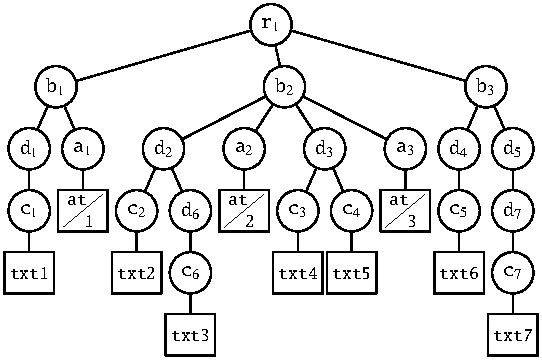
\includegraphics[scale=1.1]{partialtree/figures/bfstree.pdf}
	\caption{An example XML tree with values.}
    \label{fig:bfstree}
\end{figure}

\begin{figure}[t]
	\centering
	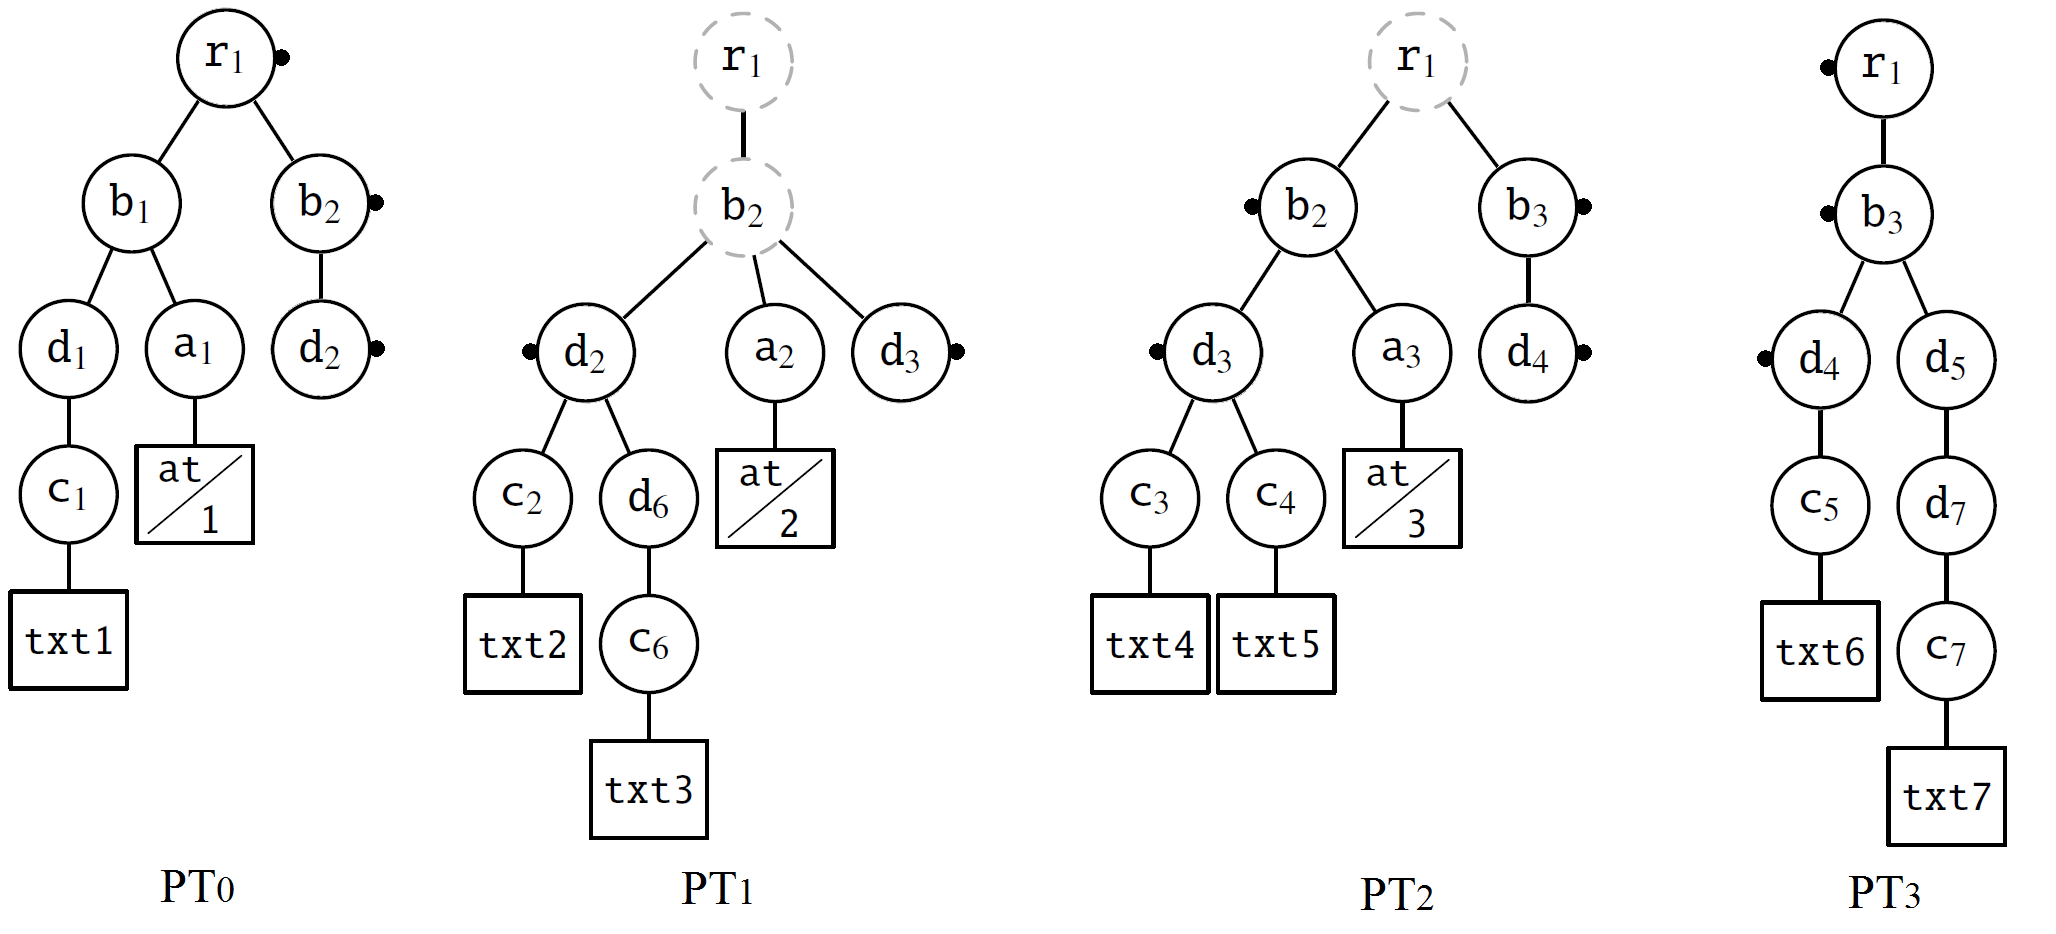
\includegraphics[scale=0.26]{partialtree/figures/bfstrees.png}
	\caption{Partial trees with values from the XML document.}
	\label{fig:bfspartialtree}
\end{figure}

For the four partial trees, we represent element nodes, attribute nodes and
value nodes consistent as the original XML tree. Since the partition only
affects the element node, from which the open nodes are only generated and
attribute nodes and content nodes can be simply implementated by the idea of
partial tree. As we have introduced in Section~\ref{sec:construction}, the split
tags are merged in case when the split position falls inside a tag and thus
splits the tag into two halves. In case of a text node is split into two sub
texts and separated on different partial trees, we simply merge the split two
sub texts into one and leave it on one partial tree. Thus this makes the
algorithm consistent.

The partial trees in the previous section provide a nice fragmentation of an XML
tree, making it possible for data parallel processing. To develop a
high-performance query framework, we still need to design concrete data
representation taking the following two issues into consideration.

\textbf{Expressiveness}

Originally indexing (or labeling) was considered to put shredded XML data into
databases~\cite{BGvM06,OOPC04}, but its expressiveness is very important to
accelerate queries.

\textbf{Compactness}

In the case we repeatedly apply several queries on the same data, we can put all
the indices in memory to avoid expensive I/O cost.

The first design choice is about the updates of XML data. In general purpose
framework, efficient support of updates is an important issues and several
frameworks support updates with sophisticated indexing such as
ORDPATH~\cite{OOPC04}. However, such an index with the update capability tends
to be large and complicated to handle. In this study, we decided not to allow
users to update XML data, which makes the implementation much simpler and
faster. We expect that users can fulfill their objective without updating the
XML data themselves,  if we provide some programming interface over the
framework.

The second design choice is about the functionality that the indices provide. An
important goal of this work is to support queries with not only the
\texttt{child} and \texttt{descendant} axes but also order-aware ones such as
\texttt{following-sibling} and \texttt{following}. To achieve our goal, the
following functions should be efficiently implemented.

\begin{figure*}[t]
	\centering
	\begin{minipage}{.2\linewidth}
		Partial tree\\[15pt]
		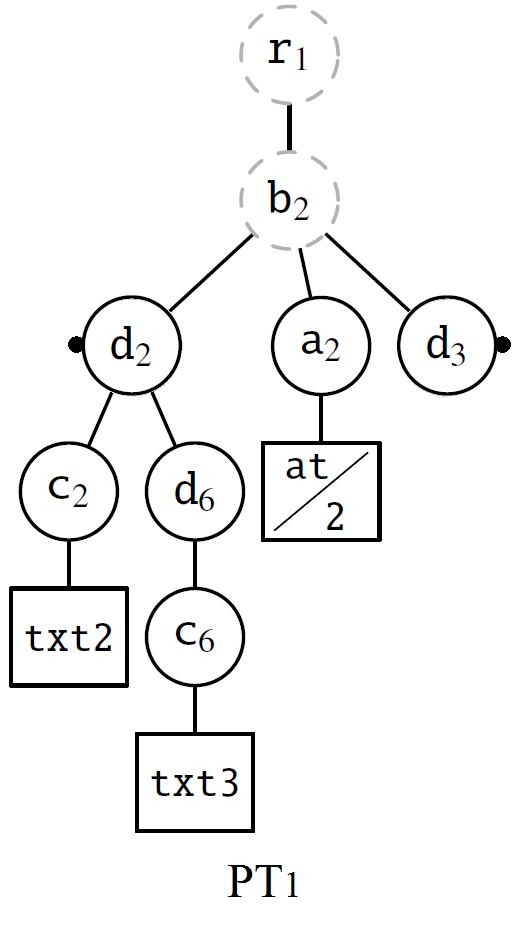
\includegraphics[scale=.25]{partialtree/figures/bfspt1.png}
	\end{minipage}
	\begin{minipage}{.55\linewidth}
		BFS-array \\
		\begin{tabular}{c|lcrrrr}
			\hline
			index   & tag             & type &  st & ed  & par    &  ch \\
			\hline
			1  & 5 (\texttt{r})  & N-OO &  0  & 196 &   0    &  2  \\
			2  & 2 (\texttt{b})  & N-OO & 42  & 142 &   1    &  3  \\
			3  & 4 (\texttt{d})  & N-OC & 45  &  81 &   2    &  6  \\
			4  & 1 (\texttt{a})  & N-CC & 81  &  95 &   2    &  8  \\
			5  & 4 (\texttt{d})  & N-CO & 95  & 124 &   2    &  9  \\
			6  & 3 (\texttt{c})  & N-CC & 48  &  59 &   3    &  9  \\
			7  & 4 (\texttt{d})  & N-CC & 59  &  77 &   3    & 10  \\
			8  & 6 (\texttt{at}) & A    & 88  &  88 &   4    & 11  \\
			9  & 0               & T    & 51  &  55 &   6    & 11  \\
			10 & 3 (\texttt{c})  & N-CC & 62  &  73 &   7    & 11  \\
			11 & 0               & T    & 65  &  69 &  10    & 12  \\
			\hline
		\end{tabular}
	\end{minipage}
    \begin{minipage} {.2\linewidth}
    Grouping Array \\[15pt]
 	\begin{tabular}{c|l}
 	\hline
 	tag  &   index      \\
 	\hline
 	0  &  $[9, 11]$ \\
 	1  &  $[4]$ \\
 	2  &  $[2]$ \\
 	3  &  $[6]$  \\
 	4  &  $[3,5,7]$  \\
 	5  &  $[1]$  \\
 	6  &  $[8]$  \\
 	\hline
    \end{tabular}
\end{minipage}
	\caption{A partial tree and its representation with two arrays}
	\label{fig:2arrays}
\end{figure*}

\begin{itemize}
	\item Function $\mathsf{getChildren}(x)$ returns all the children of node $x$.
	\item Function $\mathsf{getParent}(x)$ returns the parent of node $x$.
	\item Function $\mathsf{nextSibling}(x)$ returns the next (right) sibling of node $x$.
	\item Function $\mathsf{prevSibling}(x)$ returns the previous (left) sibling of node $x$.
	\item Function $\mathsf{isDescendant}(x, y)$ returns true if node $x$ is a descendant of node $y$.
	\item Function $\mathsf{isFollowing}(x, y)$ returns true if node $x$ is strictly after node $y$ in the document order.
	\item Function $\mathsf{getNodesIn}(t, x)$ returns all the nodes with tag $\mathit{t}$ in the subtree rooted at $x$.
\end{itemize}

We design two index sets (Fig.~\ref{fig:2arrays}) to provide these functions
keeping the indices compact. A node has the following fields:

\begin{itemize}
	\item $\mathit{tag}$: tag names (they are short integers that map to the strings),
	\item $\mathit{type}$: type of nodes including the four node types,
	\item $\mathit{st}$: start position (the position in the file to avoid global counting), and
	\item $\mathit{ed}$: end position.
\end{itemize}

The first index, \emph{BFS-array}, lists all the nodes in the order of the
breadth first search (BFS). Every node has two integer pointers to its parent
($par$) and the first child ($ch$) in this list. With the BFS order and these
two pointers, we can compute functions $\mathsf{getChildren}$,
$\mathsf{getParent}$, $\mathsf{nextSibling}$, and $\mathsf{prevSibling}$
efficiently. The second index, \emph{Grouped-array}, groups the nodes by their
tag names and then sorts the nodes in the groups by their start position.  With
this index, we can evaluate the function $\mathsf{getNodesIn}$ efficiently.

In our implementation, we used
2 bytes for $\mathit{tag}$,
1 bytes for $\mathit{type}$,
8 bytes for $\mathit{st}$,
8 bytes for $\mathit{ed}$,
4 bytes for $\mathit{par}$,
4 bytes for $\mathit{ch}$, and
4 bytes for $\mathit{idx}$.
(Though total file size could exceeds 32 bits, we assume that the number of
elements in a single partial tree can fit in 32 bits.) The total size needed for
representing a node is $2 + 1 + 8 + 8 + 4 + 4 + 4 = 31$ bytes, which is much
smaller than several implementation of DOM trees or databases. This is a key to
achieve high-performance evaluation of queries.


\section{Evaluation}
\label{sec:evaluation}

In this evaluation to our indexing, we conducted experiments for two aims: \\
1) to investigate the absolute query time with 100s GB of XML data.\\
2) to explore the scalability of our implementation on processing 
a large XML documents over a number of computing nodes.\\
We also compare ours with BaseX, the state-of-the-art XML database engine, in 
order to understand the performance of our indexing.

\subsection{Absolute Query Time} 

\subsubsection{Hardware Settings}

We used were Amazon Elastic Compute Cloud (EC2) M3 for this experiment. M3
Instances are general purpose compute instances that are powered by E5-2670 v2
(Ivy Bridge), equipped with 30 GB of memory and 2 X 80 GB of SSD, running Amazon
Linux AMI 2016.09.0. and offer a balance of compute, memory, and networking
resources for a broad range of workloads. We used m3.2xlarge instances for this
experiment, The network among EC2 instances was a local network and the network
speed is 1 gbps. The java running on m3.2xlarge was 64-Bit JVM (build
25.91-b14).


\subsubsection{Datasets and XPath Queries}

There were three datasets used in this experiment, the statistics of which are
shown in Table~\ref{tab:datasets}. For XMark datasets, we used the XML document
generator \emph{xmlgen} from XMark
project\footnote{\url{http://www.xml-benchmark.org/}}. The XMark xmlgen takes an
float number \emph{f} to determine the size of output dataset. 
For the experiments on a single EC2 instance,  we used two typical datsets: DBLP
and XMark~\cite{XMark} (with factor 100). For parallel processing, we used
XMark(with factor 2000) and UniProtKB. The UniProtKB dataset has a root element
with a large number of children with the same tag name and thus can be easily
well-formed  to be processed by multiple processors.  In contrast, XMark
datasets whose root has only six children  with different tag names, each
containing different amounts of data, makes it difficult to be well-formed.
Table 2 shows the 15 queries covering the three cases: XQ1 and UQ1 to test long
queries with nested predicates;  XQ2, DQ1, DQ2, UQ2, UQ4 and UQ5 to test
backward axes;  and the rest to test order-aware queries.

\begin{table}
	\small
	\caption{Statistics of XML dataset.}
	\label{tab:datasets}
	\begin{tabular}{c|c|c|c|c}
		\hline
		Datasets & dblp.xml & xm100.xml & xm2000.xml & uniprot.xml \\
		\hline \hline
		Nodes & 43,131,420 & 163,156,531 & 3,262,490,248 & 7,891,267,994 \\
		\hline
		Attributes & 10,885,411 & 42,257,706 & 845,072,591 & 9,254,412,578 \\
		\hline
		Values & 39,642,166 & 67,254,767 & 1,344,932,943 & 1,490,598,653 \\
		\hline
		Total & 93,658,997 & 272,669,004 & 5,452,495,782 & 18,636,279,225 \\
		\hline
		\# of tags & 47 & 77 & 77 & 82 \\
		\hline
		Size $($byte$)$ & 1,912,866,012 & 11,758,954,863 & 236,138,315,428 & 383,954,056,809 \\
		\hline
		Depth & 6 & 13 & 13 & 7 \\
		\hline
	\end{tabular}
	\vspace{10px}
	\caption{Queries used in the experiments.}
	\begin{tabular}{c|c|l}
		\hline \hline
		Name & Dataset & Query  \\
		\hline
		XQ1 & xmark & /site/closed\_auctions/closed\_auction[annotation/ \\
		&&description[text/keyword]]\\
		\hline
		XQ2 & xmark & /site//keyword/ancestor::mail \\
		\hline
		XQ3 & xmark & /site/open\_auctions/open\_auction  \\
		&&/bidder[1]/increase\\
		\hline
		XQ4 & xmark & /site/people/person/name/following-sibling::emailaddress \\
		\hline
		XQ5 & xmark & /site/open\_auctions/open\_auction[bidder\\
		&&/following-sibling::bidder]/reserve\\
		\hline
		DQ1 & dblp & /dblp//i/parent::title\\
		\hline
		DQ2 & dblp & //author/ancestor::article \\
		\hline
		DQ3 & dblp & /dblp//author/following-sibling::author \\
		\hline
		DQ4 & dblp & //author[following\textemdash sibling::author] \\
		\hline
		DQ5 & dblp & /dblp/article/title/sub/sup/i/following::author \\
		\hline
		UQ1 & uniprot & /entry[comment/text]/reference[citation \\
		&&/authorList[person]]//person\\
		\hline
		UQ2 & uniprot & /entry//fullName/parent::recommendedName \\
		\hline
		UQ3 & uniprot & /entry//fullName/following::gene \\
		\hline
		UQ4 & uniprot & //begin/ancestor::entry\\
		\hline
		UQ5 & uniprot & //begin/parent::location/parent::feature/parent::entry \\
		\hline
	\end{tabular}
\end{table}


\begin{table}[t]
	\centering
	\caption{Evaluation by one EC2 instance}
	\label{tab:singeval}
	\begin{tabular}{c|c|c|c|c|c|c|c|c|c|c}
		\hline \hline
		Dataset  & \multicolumn{5}{c|}{xmark10.xml} & \multicolumn{5}{c}{dblp.xml} \\ \hline
		Time     & \multicolumn{5}{c|}{8.5}          & \multicolumn{5}{c}{47}       \\ \hline
		Memory   & \multicolumn{5}{c|}{222}          & \multicolumn{5}{c}{3.1}       \\ \hline
		Query    & XQ1  & XQ2   & XQ3 & XQ4  & XQ5  & DQ1 & DQ2 & DQ3  & DQ4  & DQ5 \\ \hline
		Time(ms) & 591  & 1888  & 494 & 1771 & 1784 & 11  & 786 & 1863 & 3254 & 602 \\ \hline
	\end{tabular}
	\vspace{10px}
	\caption{Evaluation by multiple EC2 instance}
	\centering
	\label{tab:multieval}
	\begin{tabular}{c|c|c|c|c|c|c|c|c|c|c}
		\hline \hline
		Dataset	&	\multicolumn{5}{|c|}{xm2000.xml}     & \multicolumn{5}{c}{unirpot.xml}       \\
		\hline
		Loading (ms)	&	\multicolumn{5}{|c|}{210}     & \multicolumn{5}{c}{379}       \\
		\hline
		Memory (GB)	&	\multicolumn{5}{|c|}{173}     & \multicolumn{5}{c}{560}       \\
		\hline
		Query	& QX1      & XQ2     & QX3      & QX4      & QX5      & UX1      & UX2      & UX3      & UX4      & UX5      \\
		\hline
		Time Taken (ms) & 5951 & 819 & 1710 & 1168 & 3349 & 2573 & 2408 & 1324 & 5909 & 6220\\
		\hline
	\end{tabular}
\end{table} 

\subsection{Evaluate Queries on a Single EC2 Instance}

This experiment is to investigate the query performance on a single EC2
instance. In this case, we use the whole input XML document as a chunk and only
one partial tree generated from the chunk. Thus the queries are evaluated in
serial. The results show that for both datasets, it can process the queries
in 100s ms to several seconds. These reaults is helpful for us to understand
the query performance of partial tree in serial.


\subsection{Evaluate Queries on Multiple EC2 Instances}

In this experiment, we investigate the query performance processing 100s GB of
XML document on 32 EC2 instances. We use UniProtKB and XMark2000(f = 2000) as
experimental data. The results are shown in Table~\ref{tab:multieval}. 

In the parsing phase, for 0.545 billion and 1.86 billion elements, each of which
takes 31 bytes, the memory consumption should 157 GB and 537 GB respectively.
The experimental results show the memory consumption are 173 and 560 GB, which
are close to our analysis.  The overheads is some intermediate data generated
during construction. The parsing times as shown in Table 3 are relatively short
with regard to the data sizes. The evaluating results for XQ1 to XQ5 in Table~3
show that  the query times are just a few seconds for evaluating 220 GB and 358
GB XML data.  Besides, the loading times are just 210s and 379s.  The throughput
is around 1 GB/s. For comparison, PP-Transducer~\cite{OgTP13} achieved the best
throughput of 2.5 GB/s by using 64 cores. Although it is faster than ours, the
queries we can process are more expressive than PP-transducer, which does not
support order-aware queries.



\subsection{Scalability}
This experiment is used to explore the scalability of our indexing with up to 
64 workers.

\subsubsection{Dataset and XPath Queries} 

In our experiment, we set f to 160 and generated an 18.q54 GiB XML document
xmark160, which has 267 M element nodes, 61.3 M attribute nodes and 188 M
content nodes, totally 516.3 M nodes. We used 7 queries Q1 -- Q7 to evaluate our
implementation, including commonly used axes with predicate as  shown in
Table~\ref{tab:queries}.


\begin{table*}[ht]
	\centering
	\caption{Queries used for xmark160 dataset.}
	\label{tab:queries}
	\begin{tabular}{|l|l|l|}
		\hline
		querykey & query                                                                                  & hit nodes \\ \hline
		Q1       & /site/open\_auctions/open\_auction/bidder/increase                                     & 9577159   \\ \hline
		Q2       & /site//keyword                                                                         & 11271671  \\ \hline
		Q3       & /site//keyword/parent::text                                                            & 6503643   \\ \hline
		Q4       & /site//text{[}./keyword{]}                                                             & 6503643   \\ \hline
		Q5       & /site/people/person{[}./profile/gender{]}/name                                         & 1022629   \\ \hline
		Q6       & /site/people/person/name/following-sibling::emailaddress                               & 4080000   \\ \hline
		Q7       & /site/open\_auctions/open\_auction{[}./bidder/following-sibling::annotation{]}/reserve & 1734198   \\ \hline
	\end{tabular}
\end{table*}


\subsection{Hardware} 

The hardware we used were Amazon Elastic Compute Cloud (EC2) M5
Instances\footnote{\url{https://aws.amazon.com/ec2/instance-types/m5/}}. M5
Instances are general purpose compute instances that are powered by 2.5 GHz
Intel Xeon Scalable processors and offer a balance of compute, memory, and
networking resources for a broad range of workloads.  We used m5.2xlarge in our
experiment, which has 8 virtual cores, equipped with 32 GB of memory and
supported with solid state drives.  The instance runs Amazon Linux AMI 2018.03.0
(HVM) that supports Java by default. The Java version we used was "1.7.0\_181",
OpenJDK Runtime Environment (amzn-2.6.14.8.80.amzn1-x86\_64 u181-b00) OpenJDK
64-Bit Server VM (build 24.181-b00, mixed mode). The network among EC2 instances
was a local network and the network speed is 1 gbps.


\subsubsection{Running with a single worker}

The version of BaseX we used was 8.6.7 implemented on java 1.7. We ran it in
server/client mode. A BaseX server and a BaseX client were running on two EC2
instances. A database was created from xmark160 by the BaseX server. The server
was set in main memory mode and turned text indexing off for the creation to
make both BaseX and ours in the same setting.

To evaluate queries, we used the following XQuery expression for BaseX:  
\verb|for $node in db:open('xmark160')&query|\\
\verb|return db:node-pre($node)|, where  \verb|&query|
represents an XPath query. This expression returns a list of PRE-values and may
take a lot of time for sending and receiving among the BaseX server and a BaseX
client. Since network part is not what we are interested, we apply count() to
the results of the XPath query to both BaseX and ours so that the final outcome
will be only an integer to be returned over network, greatly removing the effect
of network.

As shown in Figure~\ref{fig:compare}, our indexing outperformances BaseX for all
the queries. Most of the queries takes only one half or one third time compared
with that of BaseX. The most significant one is Q2, for which ours is over 13
timers faster than BaseX. This is because in the two steps of Q2, \texttt{/site}
returns only 1 node, taking negligible time, while the second step,
\texttt{//keyword}, can greatly utilize the grouped-array to skip evaluating
most irrelevant nodes with different tag names as \texttt{keyword}, thus
achieving the best performance.


\begin{figure}[thb]
	\centering
	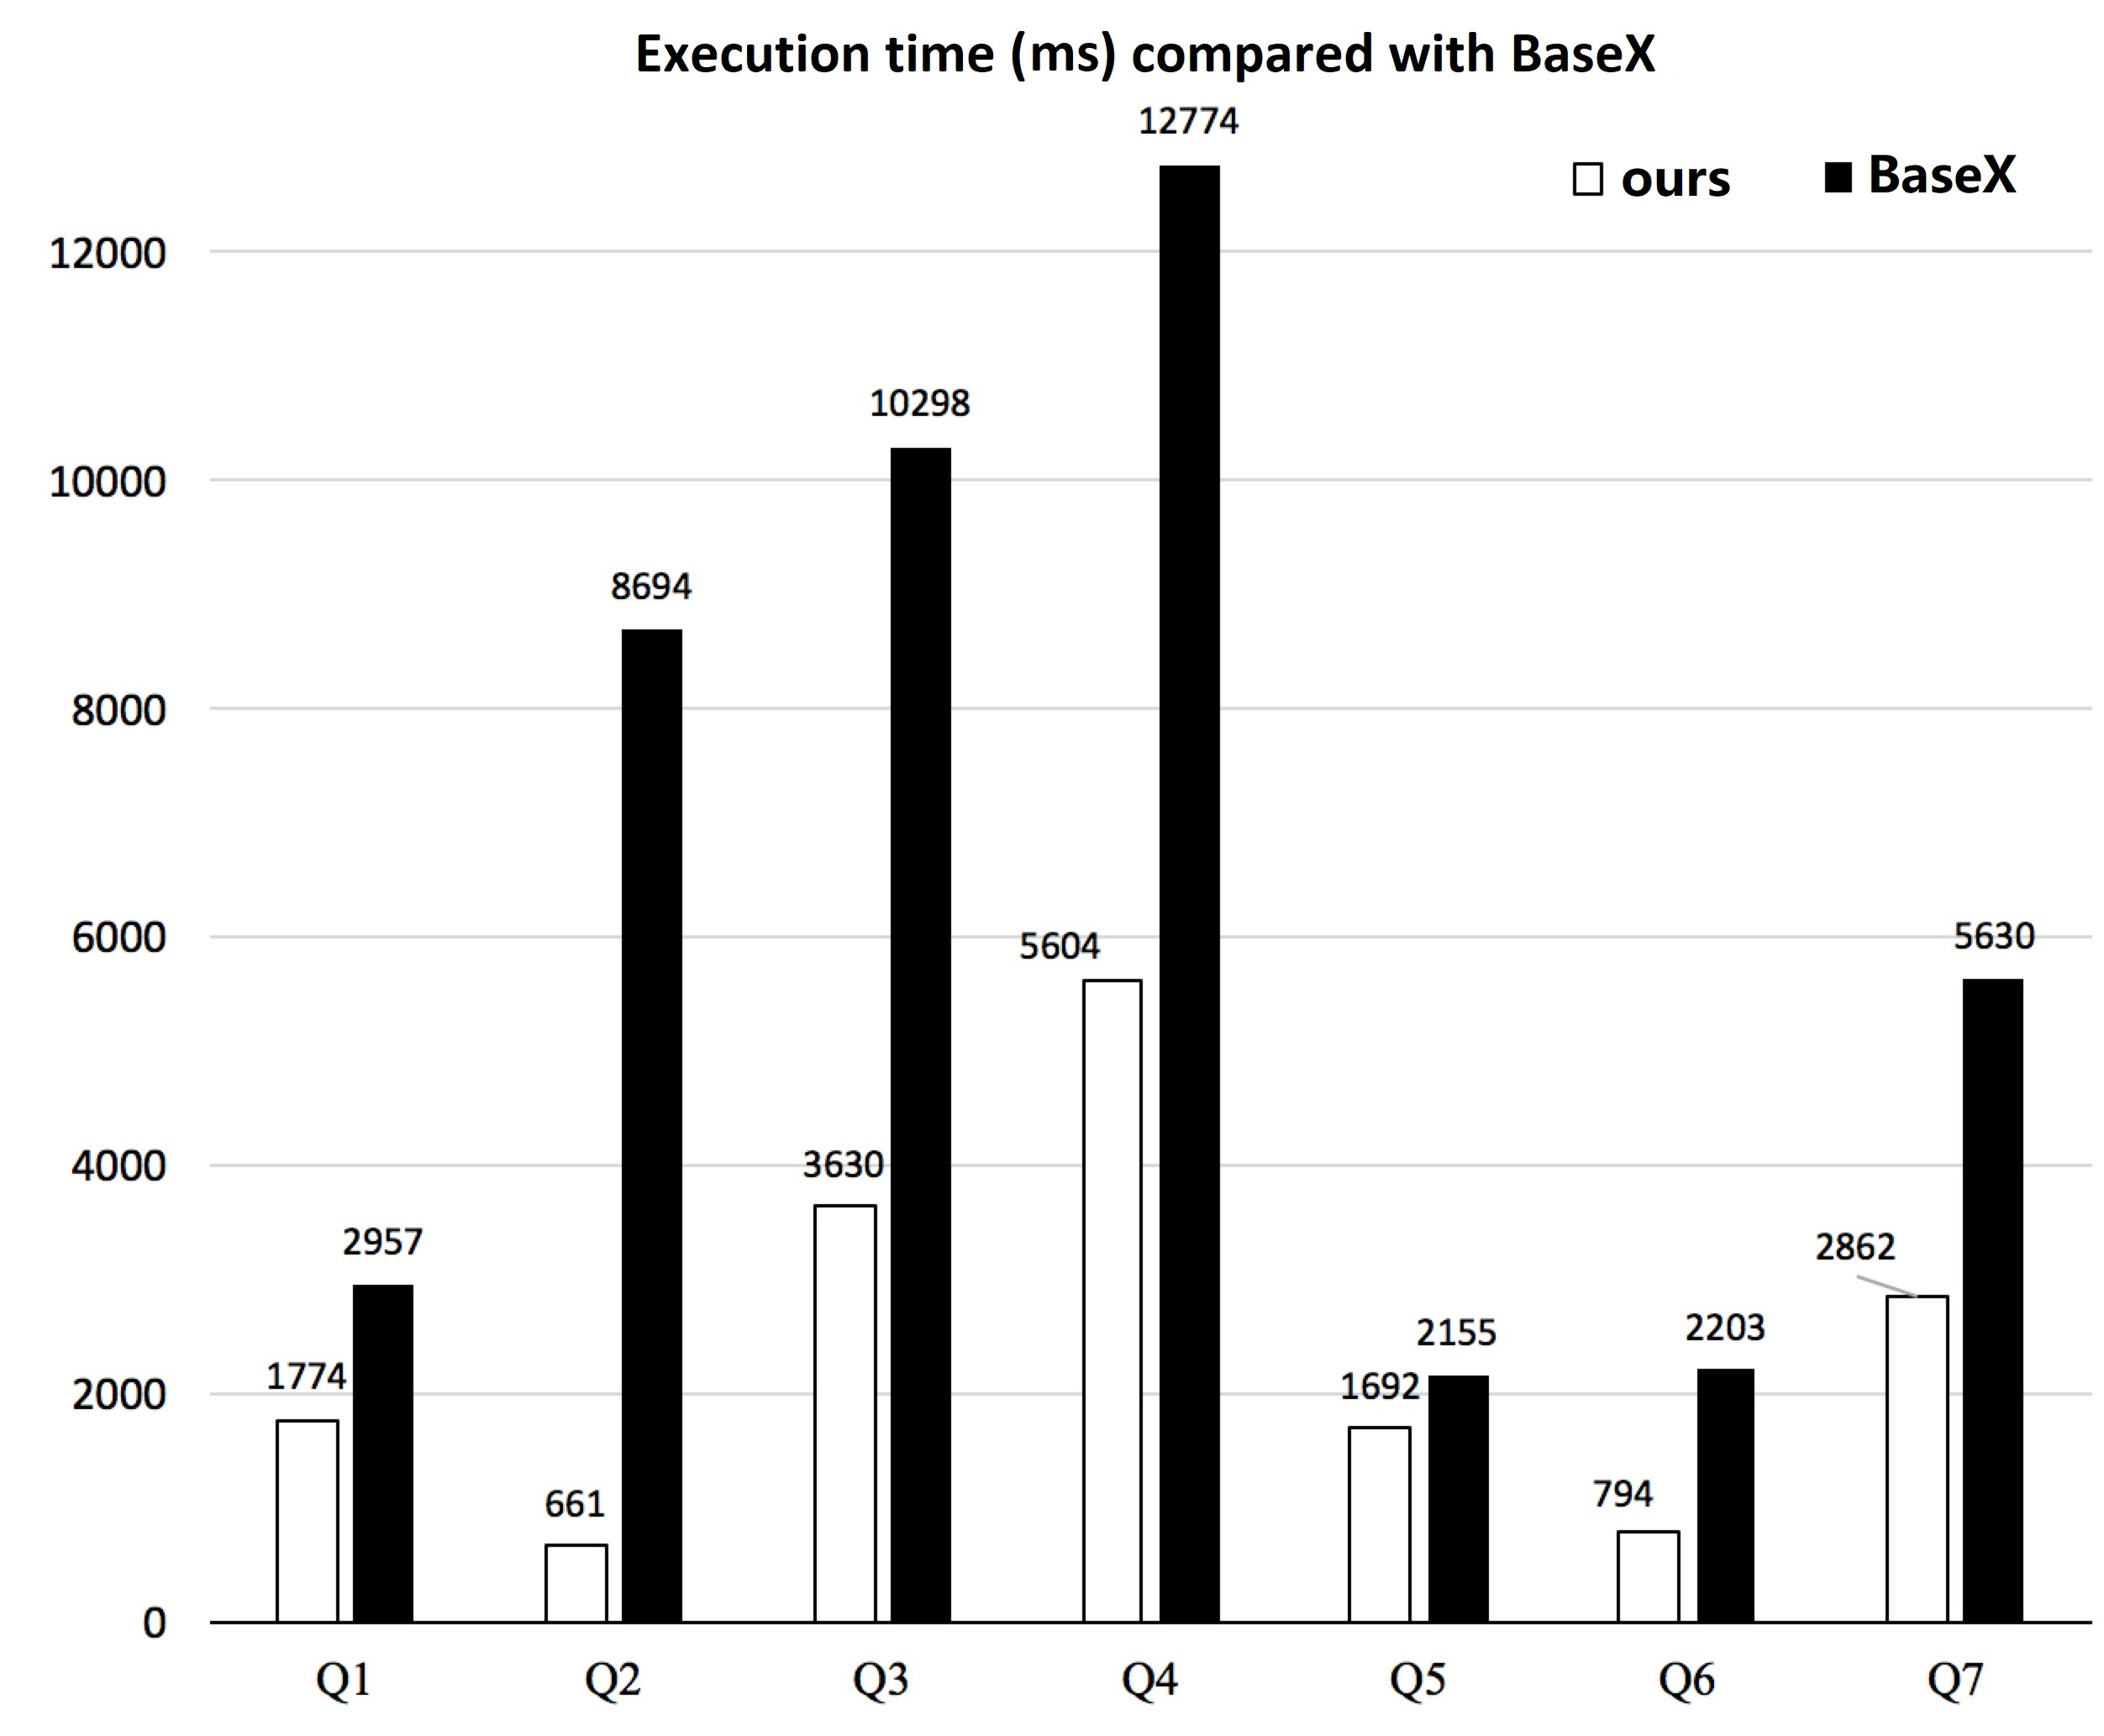
\includegraphics[width=0.9\linewidth]{compare}
	% figure caption is below the figure
	\label{fig:compare}       % Give a unique label
	\caption{Execution time (ms) compared with BaseX.}
\end{figure}

\begin{figure}[thb]
	\centering
	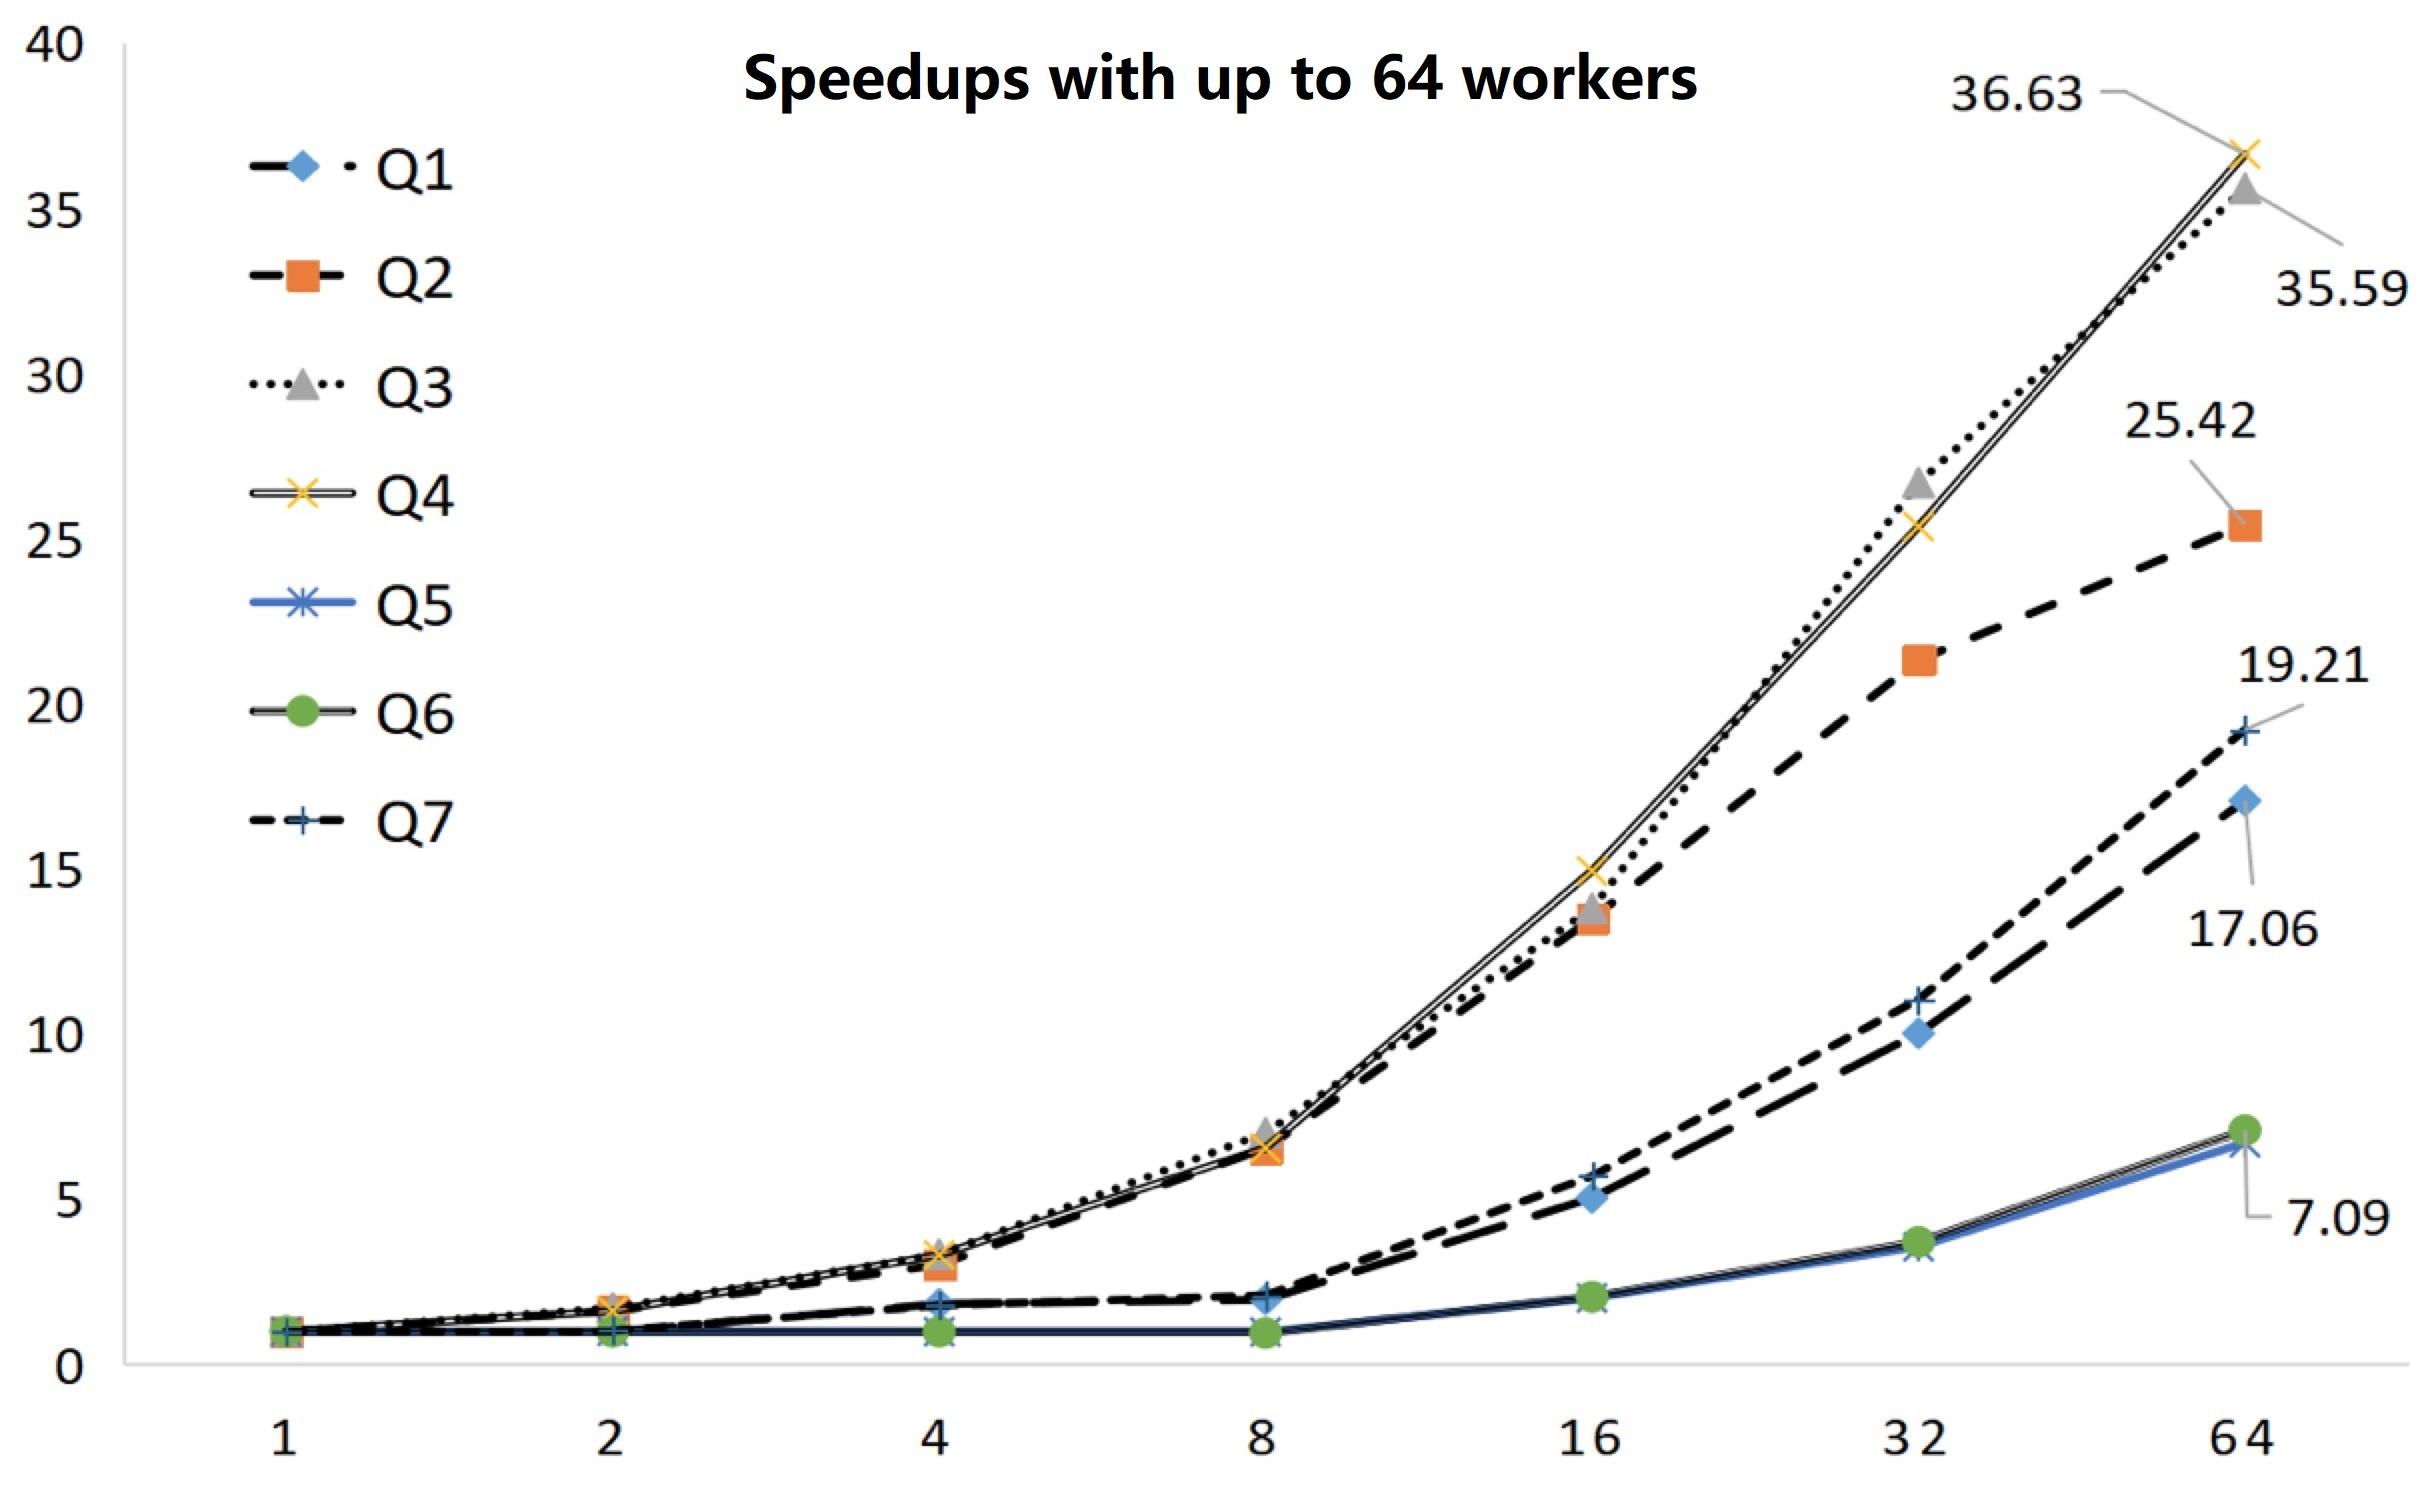
\includegraphics[width=0.9\linewidth]{speedups}
	\caption{Speedups with up to 64 workers.}
	\label{fig:speedups}    
\end{figure}


\subsubsection{Processing Queries in Parallel With Mutiple Workers}

This experiment is to test the speedups using our indexing on multiple EC2
instances. In this experiment, we use 1 instance for the master to control
query processing and 8 instances for workers to execute queries. Since the
instance m5.2xlarge has 8 cores, we arranged at most 8 workers on a single
instance. Given 8 instances, there are totally 64 workers involved in the
computation, as well as 64 chunks we divided at most. Due to the imbalance of
xmark160, not all the worker may have hit nodes of running queries. Thus, we
call workers that have hit nodes active workers, while for the rest idle
worker. 

The XML dataset xmark160 is divided into different number of chunks, to be
processed by different numbers of workers on up to 8 instances. From each chunk,
a partial tree will be created. It will be possessed and processed by a single
worker (we assign only one chunk to a worker in this experiment). 

To achieve better load balance, we used cyclic distribution to assign chunks to
instances. This means that we assign chunks to each instance, making consecutive
chunks be assigned to different instances. For example, given 8 chunks, $chunk_1$,
$chunk_2$, ..., $chunk_9$,  and 4 computing nodes, $com_1$, $com_2$, ..., $com_4$, 
we assign them as 
$com_1$($chunk_1$, $chunk_5$), 
$com_2$($chunk_2$, $chunk_6$), 
$com_3$($chunk_3$, $chunk_7$), 
$com_4$($chunk_4$, $chunk_8$). 
In such order, we can make the workers utilize the resources of computing nodes. 

We record the wall-clock time form the master's side. The timing starts from the
master sending a message to all workers to start a query, and ends at the moment
when the master receives the work-done message from the last worker, denoting
querying work is complete. The execution times are listed in
Table~\ref{tab:exetimes}.


\begin{table*}[ht]
	\centering
	\caption{Execution time in milliseconds).}
	\label{tab:exetimes}
	\begin{tabular}{|c|c|c|c|c|c|c|c|}
		\hline
		\# of workers & 1       & 2       & 4       & 8       & 16      & 32      & 64      \\ \hline
		Q1                & 1774    & 1789    & 968     & 905     & 352     & 177     & 104 \\ \hline
		Q2                & 661     & 410     & 219     & 101     &  49     & 31      & 26 \\ \hline
		Q3                & 3630    & 2120    & 1090    & 518     & 263     & 136     & 102 \\ \hline
		Q4                & 5604    & 3467    & 1695    & 855     & 375     & 221     & 153 \\ \hline
		Q5                & 1692    & 1685    & 1709    & 1731    & 841     & 475     & 252 \\ \hline
		Q6                & 794     & 800     & 803     & 834     & 388     & 214     & 112 \\ \hline
		Q7                & 2862    & 2817    & 1595    & 1369    & 502     & 259     & 149 \\ \hline
	\end{tabular}
\end{table*}

From the results, we have the following observations.

\subsubsection{Execution Time Reduced with More Workers}

From the results in the table, it is clear that with the number of workers
increased, the execution times of most queries are reduced. For
example, the execution time is nearly halves every time when the number of
workers doubled for Q3. It clearly showed that the parallel processing of
XPath queries using our index is efficient to reduce execution time by using 
more workers.

\subsubsection{Imbalance of XML Document Can Prevent Speedups}

As we can also notice, however, there are some cases execution times do not
reduce at all even with more workers. For example, no matter the number of
workers increased is 1, 2, 8 or 8, the execution times of all the cases are
still basically the same.  We analyzed the number of active workers and found
that this is caused by the imbalance of XMark datasets. In the xmark160, the hit
nodes of queries may only reside on a consecutive part of the XML document.
Then, after being divided, the hit nodes may be distributed in a small number of
chunks. Thus, only the workers that possess these chunks can be active, while
the rest workers just stay idle. Let us continue to take Q5 as an example. When
the number of workers increases from 1 to 8, the number of active nodes,
however, does not increase and still stays 1, i.e. there was only one active
worker for the query. Therefore, with only one worker, it takes nearly the same
amount of time to process the same amount of hit nodes regardless how many
workers were totally used. 

\subsubsection{Imbalance of XML Document Can Spoil Speedups}

We also notice that some execution times are not reduced much when even when
more active workers involve. For example, Q2 takes 661 ms by one active worker
and 410 ms for two active workers, the execution is not halved. This is because
the hit nodes did not evenly distributed over the two active workers. As we
investigated, one worker took 406 ms to collect 6785094 hit nodes, while another
worker took 256 ms for 4486577 hit nodes. Therefore, the speedup is degraded due
to the imbalanced distribution of hit nodes over chunks. We can learn that the
imbalance can not only prevent the speedup, but also can degrade the speedup.

To understand how much speedup ours can achieve, we use the execution time done
by a single worker as baseline. The results are shown in
Figure~\ref{fig:speedups}.  From the figure, it shows that ours can achieve
better speedup when using more workers. The best speed up is done from Q3 by a
factor of 36.63. We also notice that when the number of workers are large than
8, the speedup becomes dramatical, which means with more chunks divided, the
imbalance can be smoothed and it can be more effective for better speedups. This
is because  with smaller chunks, hit nodes can be distributed to more chunks;
meanwhile,  with the cyclic distribution of these small chunks, we can have more
active workers to participate in the querying process, thus achieving better
speedups. 


\subsubsection{Discussion}

From the experiment results and our analysis in previous sub section, we suggest
that it is better to assign more chunks to a worker rather than one as what we
conducted in the experiment. In such case, more workers will possess chunks that
contain hit nodes. In ideal case, hit nodes consecutively contained in a part of
the XML document can be divided into more chunks, and these chunks can be
distributed to each of workers.  Then, all the workers become active and we can
achieve better speedups. However, with too many chunks, it is not clear how
much overhead on memory, thread or network etc will be involved. We need to find
a trade-off about the maxamum number of chunks to reach the best performance.
Thus, it is worth studying for the future work.



 

%\section{Summary}

In this chapter, we have first developed a novel tree structure called partial
tree based on a vertical fragmentation of XML documents. To construct partial
trees from an XML document, there are four phases. First, we split the XML
document into several chunks. Second, we parse the chunks in parallel to form
several sets of subtrees that have some open nodes. Third, we compute pre-paths
from all open nodes. Last, we put pre-paths to each corresponding set of
subtrees to complete the partial tree construction.

After the introduction to partial tree, we have also designed query algorithms
for most useful class of XPath queries with three examples to demonstrate how
the query algorithms work.

Last, we have implemented partial tree with a BFS-array based index for high-
efficiency. The experiment shows that the implementation reaches a good absolute
query time that can evaluate XPath queries over 100s GB of XML documents in 100s
millisecond to several seconds.



\chapter{Conclusion and Future Work}

This thesis has investigated the parallelization of XPath queries on large XML
documents with two approaches, BaseX and partial tree. We conclude our thesis in
this chapter.

\section{Conclusion}

Parallelization of XPath queries on XML documents has been studied in the past
decade. Most of these studies either focused a small set of XPath queires or
were not practical for large XML documents. Thus these studies cannot meet the
requirements of the rapid grow of XML documents.

To overcome the difficulties, we first revived an existing study proposed by
Bordawerker et al. in 2008. Their work was implemented on Xalan, which is a XSLT
processor and has already been out of date now because the hardware and software
have both changed. We presented our three implementations on top of a
state-of-the-art XML databasex engine BaseX over XML documents sized server
gigabytes. Since BaseX provides full support for XQuery/XQuery 3.1, we can
harness this feature to process subqueries from the division of target XPath
queries.

Through our implementations, we are the first to experimentally prove that it is
possible to obtain significant speedups by simply rewriting queries into
subqueries and parallelizing the evaluation of them on top of an XML database
engine over gigabytes of XML documents, without need to modify source code of
the engine. From the experimental evaluation, our implementations exhibited a
great advantage that we are able to use off-the-shelf XML database engines to
parallelize the evalaution of XPath queries over gigabytes XML documents, which
is very convinient and practical.

For processing larger XML documents, we proposed a novel tree, called partial
tree. With partial tree, we extend the processing of XML documents from
shared-memory environments to distributed-memory environments, making it
possible to utilize computer clusters. We also proposed an efficient BFS-array
based implementation of partial tree. The experiment results showed the
efficiency of our framework that the implementation are able to process 100s GB
of XML documents with 32 EC2 computers. The execution times were only seconds
for most queries used in the experiments and the throughput was approximately 1
GB/s. There is only one known study that reached faster throughput than ours,
which was 2.5 GB/s with 64 cores. However, ours can support more complicated
queries, such as order-aware queries, thus making our approach more expressive.

Besides the throughput, partial tree also has the following two good features.
First, it is practical to evenly divide an large XML document and create partial
trees out of the similar size so that we can reach good load-balancing. Second,
partial trees are portable in both shared-/distributed- memory environemts. This
means that we can make them work in both distributed-memory environments and
shared-memory environments, without changing the setting of partial tree.
Therefore, partial tree is a promising data structure and helpful for parallel
XML processing, especially for large XML documents in distributed-memory
environments.

\section{Future Work}

Based on the studies of BaseX and the partial tree, there are three works that
are worthing doing in the future.

Firstly, our implementations on top of BaseX were evaluated with only a single
BaseX server on a dual-CPU system. Thus, it would be very promising to use
multiple BaseX servers on multiple CPUs in distributed-memory environments over
large XML documents. Considering the PRE values that are integers and very
small, it is suitable to represent the intermediate results of queries by PRE
values to be transmitted among BaseX processors. With more BaseX servers running
on a computer cluster, it is feasible to efficiently process larger XML
documents.

Secondly, although partial trees are suitable for processing XPath queires over
large XML documents, the functionality and fault tolerance, which are both
important for process large XML documents, are still weak when partial trees
work alone. Therefore, developing a partial tree based framework that cooperates
with the distributed systems such as MapReduce or similar frameworks would be a
good designing choice. Also, equipping additional programming interfaces to
handle more complicated queries or larger data is practically important for the
framework.

Lastly, the application of partial tree to BaseX would also be an interesting
work. By the introduction of partial tree into BaseX, we can exploit good
features of partial tree, such as handling imbalanced trees. In this way, it is
high likely to achieve good scalability, especially in case of the
implementation of BaseX in distributed-memory environments.


\begin{declaration}
	
	I herewith declare that I have produced this paper without the prohibited
	assistance of third parties and without making use of aids other than those
	specified; notions taken over directly or indirectly from other sources have
	been identified as such. This paper has not previously been presented in
	identical or similar form to any other Japan or foreign examination board.
	
	The thesis work was conducted from Wei HAO under the supervision of Associate
	Professor Kiminori Matsuzaki at Kochi University of Technology, Kami City, Kochi
	Prefecture, Japan.
	
	\vspace{70mm}
	
	\hspace{80mm} Signature:
	
	\hspace{80mm} Date:
	
\end{declaration}




%: ----------------------- bibliography ------------------------
\bibliographystyle{ieeetr}
\bibliography{backmatter/references}


\begin{declaration}
	
	I herewith declare that I have produced this paper without the prohibited
	assistance of third parties and without making use of aids other than those
	specified; notions taken over directly or indirectly from other sources have
	been identified as such. This paper has not previously been presented in
	identical or similar form to any other Japan or foreign examination board.
	
	The thesis work was conducted from Wei HAO under the supervision of Associate
	Professor Kiminori Matsuzaki at Kochi University of Technology, Kami City, Kochi
	Prefecture, Japan.
	
	\vspace{70mm}
	
	\hspace{80mm} Signature:
	
	\hspace{80mm} Date:
	
\end{declaration}



\end{document}
